\chapter{Classification of Matter - Grade 10}
\label{chap:classification}

All the objects that we see in the world around us, are made of \textbf{matter}. Matter makes up the air we breathe, the ground we walk on, the food we eat and the animals and plants that live around us. Even our own human bodies are made of matter!\\

Different objects can be made of different types of matter, or \textbf{materials}. For example, a cupboard (an \textit{object}) is made of wood, nails and hinges (the \textit{materials}). The \textbf{properties} of the materials will affect the properties of the object. In the example of the cupboard, the strength of the wood and metals make the cupboard strong and durable. In the same way, the raincoats that you wear during bad weather, are made of a material that is waterproof. The electrical wires in your home are made of metal because metals are a type of material that is able to conduct electricity. It is very important to understand the properties of materials, so that we can use them in our homes, in industry and in other applications. In this chapter, we will be looking at different types of materials and their properties.\\

The diagram below shows one way in which matter can be classified (grouped) according to its different properties. As you read further in this chapter, you will see that there are also other ways of classifying materials, for example according to whether they are good electrical conductors.

%Start of Code
\begin{figure}[!ht]
\begin{center}
\begin{pspicture}(-6,0.5)(6,5)
%\psgrid[gridcolor=lightgray]
\rput(0,4.8){\textbf{MATTER}}
\psline(-3,4)(-3,4.4)(3,4.4)(3,4)
\rput(-3,3.8){\textbf{MIXTURES}}
\rput(3,3.8){\textbf{PURE SUBSTANCES}}
\psline(-3,3.4)(-3,3.6)
\psline(3,3.4)(3,3.6)
\psline(-4.5,3)(-4.5,3.4)(-1.5,3.4)(-1.5,3)
\psline(4.5,3)(4.5,3.4)(1.5,3.4)(1.5,3)
\rput(-4.5,2.8){Homogeneous}
\rput(-1.5,2.8){Heterogeneous}
\rput(4.5,2.8){Compounds}
\rput(1.5,2.8){Elements}
\psline(1.5,2.6)(1.5,2.4)
\psline(0,2.0)(0,2.4)(3,2.4)(3,2.0)
\rput(0,1.8){Metals}
\rput(3,1.8){Non-metals}
\psline(0,1.4)(0,1.6)
\psline(-1.5,1.2)(-1.5,1.4)(1.5,1.4)(1.5,1.2)
\rput(-1.5,1){Magnetic}
\rput(1.5,1){Non-magnetic}
%\psset{yunit=0.5}
\end{pspicture}
\caption{The classification of matter}
\label{fig:c:ClassificationOfMatter}
\end{center}
\end{figure}
%End of code


% CHILD SECTION START 

\section{Mixtures}
\label{sec:cm:mps}

We see mixtures all the time in our everyday lives. A stew, for example, is a mixture of different foods such as meat and vegetables; sea water is a mixture of water, salt and other substances, and air is a mixture of gases such as carbon dioxide, oxygen and nitrogen. 

\Definition{Mixture}{A \textbf{mixture} is a combination of more than one substance, where these substances are not bonded to each other.} 

In a mixture, the substances that make up the mixture:

\begin{itemize}
\item{\textit{are not in a fixed ratio}

Imagine, for example, that you have a 250 ml beaker of water. It doesn't matter whether you add 20 g, 40 g, 100 g or any other mass of sand to the water; it will still be called a mixture of sand and water.}

\item{\textit{keep their physical properties}

In the example we used of the sand and water, neither of these substances has changed in any way when they are mixed together. Even though the sand is in water, it still has the same properties as when it was out of the water.}

\item{\textit{can be separated by mechanical means}

To separate something by 'mechanical means', means that there is no chemical process involved. In our sand and water example, it is possible to separate the mixture by simply pouring the water through a filter. Something \textit{physical} is done to the mixture, rather than something \textit{chemical}.} 
\end{itemize}

Some other examples of mixtures include blood (a mixture of blood cells, platelets and plasma), steel (a mixture of iron and other materials) and the gold that is used to make jewellery. The gold in jewellery is not pure gold but is a mixture of metals. The \textit{carat} of the gold gives an idea of how much gold is in the item.\\ 

We can group mixtures further by dividing them into those that are heterogeneous and those that are homogeneous.

\subsection{Heterogeneous mixtures}

A \textbf{heterogeneous} mixture does not have a definite composition. Think of a pizza, that is a mixture of cheese, tomato, mushrooms and peppers. Each slice will probably be slightly different from the next because the toppings like the mushrooms and peppers are not evenly distributed. Another example would be granite, a type of rock. Granite is made up of lots of different mineral substances including quartz and feldspar. But these minerals are not spread evenly through the rock and so some parts of the rock may have more quartz than others. Another example is a mixture of oil and water. Although you may add one substance to the other, they will stay separate in the mixture. We say that these heterogeneous mixtures are \textit{non-uniform}, in other words they are not exactly the same throughout.  

\Definition{Heterogeneous mixture}{A heterogeneous mixture is one that is non-uniform, and where the different components of the mixture can be seen.}

\subsection{Homogeneous mixtures}

A \textbf{homogeneous} mixture has a definite composition, and specific properties. In a homogeneous mixture, the different parts cannot be seen. A solution of salt dissolved in water is an example of a homogeneous mixture. When the salt dissolves, it will spread evenly through the water so that all parts of the solution are the same, and you can no longer see the salt as being separate from the water. Think also of a powdered drink that you mix with water. Provided you give the container a good shake after you have added the powder to the water, the drink will have the same sweet taste for anyone who drinks it, it won't matter whether they take a sip from the top or from the bottom. The air we breathe is another example of a homogeneous mixture since it is made up of different gases which are in a constant ratio, and which can't be distinguished from each other.

\Definition{Homogeneous mixture}{A homogeneous mixture is one that is uniform, and where the different components of the mixture cannot be seen.}

An \textbf{alloy} is a homogeneous mixture of two or more elements, at least one of which is a metal, where the resulting material has metallic properties. Alloys are usually made to improve on the properties of the elements that make them up. Steel for example, is much stronger than iron, which is its main component.

\subsection{Separating mixtures}

Sometimes it is important to be able to separate a mixture. There are lots of different ways to do this. These are some examples:

\begin{itemize}

\item{\textit{Filtration}

A piece of filter paper in a funnel can be used to separate a mixture of sand and water.}

\item{\textit{Heating / evaporation}

Sometimes, heating a solution causes the water to evaporate, leaving the other part of the mixture behind. You can try this using a salt solution.}

\item{\textit{Centrifugation}

This is a laboratory process which uses the centrifugal force of spinning objects to separate out the heavier substances from a mixture. This process is used to separate the cells and plasma in blood. When the test tubes that hold the blood are spun round in the machine, the heavier cells sink to the bottom of the test tube. Can you think of a reason why it might be important to have a way of separating blood in this way?}

\item{\textit{Dialysis}

This is an interesting way of separating a mixture because it can be used in some important applications. Dialysis works using a process called \textit{diffusion}. Diffusion takes place when one substance in a mixture moves from an area where it has a high concentration to an area where its concentration is lower. When this movement takes place across a semi-permeable membrane it is called osmosis. A semi-permeable membrane is a barrier that lets some things move across it, but not others. This process is very important for people whose kidneys are not functioning properly, an illness called \textit{renal failure}.} 
\end{itemize}

\begin{IFact}
{Normally, healthy kidneys remove waste products from the blood. When a person has renal failure, their kidneys cannot do this any more, and this can be life-threatening. Using dialysis, the blood of the patient flows on one side of a semi-permeable membrane. On the other side there will be a fluid that has no waste products but lots of other important substances such as potassium ions ($K^{+}$) that the person will need. Waste products from the blood diffuse from where their concentration is high (i.e. in the person's blood) into the 'clean' fluid on the other side of the membrane. The potassium ions will move in the opposite direction from the fluid into the blood. Through this process, waste products are taken out of the blood so that the person stays healthy.}
\end{IFact}

\Activity{Investigation}{The separation of a salt solution\\}{

\textbf{Aim:}\\

To demonstrate that a homogeneous salt solution can be separated using physical methods.\\

\textbf{Apparatus:}\\

glass beaker, salt, water, retort stand, bunsen burner.\\

\textbf{Method:}

\begin{enumerate}
\item{Pour a small amount of water (about 20 ml) into a beaker.}
\item{Measure a teaspoon of salt and pour this into the water.}
\item{Stir until the salt dissolves completely. This is now called a \textit{salt solution}. This salt solution is a homogeneous mixture.}
\item{Place the beaker on a retort stand over a bunsen burner and heat gently. You should increase the heat until the water almost boils.}
\item{Watch the beaker until all the water has evaporated. What do you see in the beaker? }
\end{enumerate}


\begin{center}
\begin{pspicture}(0,-0.5)(8,5.5)
\SpecialCoor
%\psgrid%[gridcolor=lightgray]
\rput(0,0){\stand}
\rput(0.5,2.5){\filledbeaker}
\rput(0.5,0){\bunsen}
\uput[u](1.2,3){salt}
\rput(1.2,3){solution}

\rput(4,0){
\rput(0,0){\stand}
\degrees[1.1]
\rput(0.5,2.5){\filledbeaker
\multido{\n=0.0+0.1}{3}{\multirput{10}(0.2,\n)(0.1,0){12}{\psframe(0,0)(0.1,0.1)}}
}

\rput(0.5,0){\bunsen}
\uput[r](1,3.5){H$_2$O}
\psline{->}(1,2.95)(1,3.95)
}

\psline(2.6,2)(2.1,2)\rput(3.2,2){stand}\psline(3.8,2)(4.4,2)
\uput[u](3.2,0.8){bunsen}
\psline(2.6,0.8)(1.4,0.8)\rput(3.2,0.8){burner}\psline(3.8,0.8)(5,0.8)

\uput[ur](6.5,4){water evaporates}
\uput[ur](6.5,3.8){when the solution}
\uput[dr](6.5,4){is heated}

\uput[ur](6.5,2.6){salt crystals}
\uput[ur](6.5,2.4){remain at the}
\uput[dr](6.5,2.6){bottom of the beaker}

\end{pspicture}
\end{center}

\textbf{Results:}\\

The water evaporates from the beaker and tiny grains of salt remain at the bottom.\\

\textbf{Conclusion:}\\

The sodium chloride solution, which was a homogeneous mixture of salt and water, has been separated using heating and evaporation. 

}

\Activity{Discussion}{Separating mixtures\\}{\textit{Work in groups of 3-4}

Imagine that you have been given a container which holds a mixture of sand, iron filings (small pieces of iron metal), salt and small stones of different sizes. Is this a homogeneous or a heterogeneous mixture? In your group, discuss how you would go about separating this mixture into the four materials that it contains.}

\Exercise{Mixtures\\}{
\begin{enumerate}
\item{Which of the following subtances are \textit{mixtures}?

	\begin{enumerate}
	\item{tap water}
	\item{brass (an alloy of copper and zinc)}
	\item{concrete}
	\item{aluminium}
	\item{Coca cola}
	\item{distilled water}
	\end{enumerate}
}

\item{In each of the examples above, say whether the mixture is homogeneous or heterogeneous}

\end{enumerate}
}


% CHILD SECTION END 



% CHILD SECTION START 

\section{Pure Substances: Elements and Compounds}
\label{sec:class:pure}

Any material that is not a mixture, is called a \textbf{pure substance}. Pure substances include \textbf{elements} and \textbf{compounds}. It is much more difficult to break down pure substances into their parts, and complex chemical methods are needed to do this.

\subsection{Elements}

An \textbf{element} is a chemical substance that can't be divided or changed into other chemical substances by any ordinary chemical means. The smallest unit of an element is the \textbf{atom}. 

\Definition{Element}{An element is a substance that cannot be broken down into other substances through chemical means.}

There are 112 officially named elements and about 117 known elements. Most of these are natural, but some are man-made. The elements we know are represented in the \textbf{Periodic Table of the Elements}, where each element is abbreviated to a \textbf{chemical symbol}. Examples of elements are magnesium (Mg), hydrogen (H), oxygen (O) and carbon (C). On the Periodic Table you will notice that some of the abbreviations do not seem to match the elements they represent. The element iron, for example, has the chemical formula Fe. This is because the elements were originally given Latin names. Iron has the abbreviation Fe because its Latin name is 'ferrum'. In the same way, sodium's Latin name is 'natrium' (Na) and gold's is 'aurum' (Au).

\subsection{Compounds}

A \textbf{compound} is a chemical substance that forms when two or more elements combine in a fixed ratio. Water (H$_{2}$O), for example, is a compound that is made up of two hydrogen atoms for every one oxygen atom. Sodium chloride (NaCl) is a compound made up of one sodium atom for every chlorine atom. An important characteristic of a compound is that it has a \textbf{chemical formula}, which describes the ratio in which the atoms of each element in the compound occur.

\Definition{Compound}{A substance made up of two or more elements that are joined together in a fixed ratio.}

Diagram \ref{fig:classification:mixture and compound} might help you to understand the difference between the terms \textit{element}, \textit{mixture} and \textit{compound}. Iron (Fe) and sulfur (S) are two elements. When they are added together, they form a \textit{mixture} or iron and sulfur. The iron and sulfur are not joined together. However, if the mixture is heated, a new \textit{compound} is formed, which is called iron sulfide (FeS). In this compound, the iron and sulfur are joined to each other in a ratio of 1:1. In other words, one atom of iron is joined to one atom of sulfur in the compound iron sulfide.

\begin{figure}[h]
\begin{center}
\begin{pspicture}(0,-1)(11,4.7)
\SpecialCoor
%\psgrid[gridcolor=lightgray]
\def\fe{\pscircle[fillcolor=lightgray,fillstyle=solid](0,0){0.4}\rput(0,0){Fe}}
\def\s{\pscircle[fillcolor=white,fillstyle=solid](0,0){0.2}\rput(0,0){S}}
\def\fes{\fe \rput(0.6,0){\s}} 

\psframe(0,0)(4,4)
\rput(1.5,2){\s}
\rput{30}(3,1){\rput(1,1){\fe}\rput(1.5,2){\s}}
\rput{65}(1.55,1.33){\rput(1,1){\fe}\rput(1.5,2){\s}}
\rput{265}(2,3){\rput(-0.5,0.6){\fe}\rput(1.5,1.6){\s}}
\rput(2,0.6){\s}
\rput(1,1){\fe}
\rput(3,0.7){\fe}
\rput(2.4,2){\fe}
\rput(1.4,3.6){\s}
\psline(3.4,0.6)(4.2,0.6)
\uput[r](4.2,0.6){\parbox{1.5cm}{An atom of the element iron (Fe)}}

\psline(3.5,3.5)(4.2,3.5)
\uput[r](4.2,3.5){\parbox{1.5cm}{An atom of the element sulfur (S)}}
\rput(2,-0.5){\parbox{4cm}{A mixture of iron and sulfur}}

\rput(7,0){
\psframe(0,0)(4,4)
\rput{30}(1,2){\fes}
\rput{45}(1,1){\fes}
\rput{90}(3,0.7){\fes}
\rput{245}(1,3.5){\fes}
\rput{190}(3,3.2){\fes}
\rput{60}(2.4,2){\fes}
\rput(2,-0.5){\parbox{4cm}{The compound iron sulfide (FeS)}}
}

\end{pspicture}
\end{center}
\caption{Understanding the difference between a mixture and a compound}
\label{fig:classification:mixture and compound}
\end{figure}

\Exercise{Elements, mixtures and compounds\\}{

\begin{enumerate}

\item{In the following table, tick whether each of the substances listed is a \textit{mixture} or a \textit{pure substance}. If it is a mixture, also say whether it is a homogeneous or heterogeneous mixture.\\

\begin{center}
\begin{tabular}{|p{3cm}|p{3cm}|p{3cm}|}\hline
\textbf{Substance} & \textbf{Mixture or pure} & \textbf{Homogeneous or heterogeneous mixture}\\\hline
fizzy colddrink &  &  \\\hline
steel & & \\\hline
oxygen & & \\\hline
iron filings & & \\\hline
smoke & & \\\hline
limestone ($CaCO_{3}$) & & \\\hline

\end{tabular}
\end{center}
}

\item{In each of the following cases, say whether the substance is an element, a mixture or a compound.
	\begin{enumerate}
	\item{Cu}
	\item{iron and sulfur}
	\item{Al}
	\item{H$_{2}$SO$_{4}$}
	\item{SO$_{3}$}
	\end{enumerate}
}
\end{enumerate}
}


% CHILD SECTION END 



% CHILD SECTION START 

\section{Giving names and formulae to substances}

It is easy to describe elements and mixtures. But how are compounds named? In the example of iron sulfide that was used earlier, which element is named first, and which 'ending' is given to the compound name (in this case, the ending is -ide)?

The following are some guidelines for naming compounds:

\begin{enumerate}

\item{The compound name will always include the \textbf{names of the elements} that are part of it.}

	\begin{itemize}
	\item{A compound of \textbf{iron} (Fe) and \textit{sulfur} (S) is \textbf{iron} \textit{sulf}ide (FeS)}
	\item{A compound of \textbf{potassium} (K) and \textit{bromine} (Br) is \textbf{potassium} \textit{brom}ide (KBr)}
	\item{A compound of \textbf{sodium} (Na) and \textit{chlorine} (Cl) is \textbf{sodium} \textit{chlor}ide (NaCl)}
	\end{itemize}

\item{In a compound, the element that is on the left of the Periodic Table, is used \textit{first} when naming the compound. In the example of NaCl, sodium is a group 1 element on the left hand side of the table, while chlorine is in group 7 on the right of the table. Sodium therefore comes first in the compound name. The same is true for FeS and KBr.}

\item{The \textbf{symbols} of the elements can be used to represent compounds e.g. FeS, NaCl and KBr. These are called \textbf{chemical formulae}. In these three examples, the ratio of the elements in each compound is 1:1. So, for FeS, there is one atom of iron for every atom of sulfur in the compound.}

\item{A compound may contain \textbf{compound ions}. An ion is an atom that has lost (positive ion) or gained (negative ion) electrons. Some of the more common compound ions and their names are shown below.

\begin{center}
\begin{tabular}{|l|l|}\hline
Name of compound ion & formula\\\hline
Carbonate & CO$_3$$^2$$^-$\\\hline
Sulfate & SO$_4$$^2$$^-$\\\hline
Hydroxide & OH$^-$\\\hline
Ammonium & NH$_{4}$$^{+}$\\\hline
Nitrate & NO$_{3}$$^{-}$\\\hline
Hydrogen carbonate & HCO$_3$$^-$\\\hline
Phosphate & PO$_{4}$$^{3-}$\\\hline
Chlorate & ClO$_{3}$$^{-}$\\\hline
Cyanide & CN$^{-}$\\\hline
Chromate & CrO$_{4}$$^{2-}$\\\hline
Permanganate & MnO$_{4}$$^{-}$\\\hline
\end{tabular}
\end{center}
}

\item{When there are only two elements in the compound, the compound is often given a \textbf{suffix} (ending) of -ide. You would have seen this in some of the examples we have used so far. For compound ions, when a non-metal is combined with oxygen to form a negative ion (anion) which then combines with a positive ion (cation) from hydrogen or a metal, then the suffix of the name will be ...ate or ...ite. NO$_{3}^{-}$ for example, is a negative ion, which may combine with a cation such as hydrogen (HNO$_{3}$) or a metal like potassium (KNO$_{3}$). The NO$_{3}^{-}$ anion has the name nitr\textbf{ate}. SO$_{3}^{2-}$ in a formula is sulph\textbf{ite}, e.g. sodium sulfite (Na$_{2}$SO$_{3}$). SO$_{4}^{2-}$ is sulf\textbf{ate} and PO$_{4}^{3-}$ is phosph\textbf{ate}. 
}

\item{\textbf{Prefixes} can be used to describe the ratio of the elements that are in the compound. You should know the following prefixes: 'mono' (one), 'di' (two) and 'tri' (three).}

	\begin{itemize}
	\item{CO (carbon monoxide) - There is one atom of oxygen for every one atom of carbon}
	\item{NO$_{2}$ (nitrogen dioxide) - There are two atoms of oxygen for every one atom of nitrogen}
	\item{SO$_{3}$ (sulfur trioxide) - There are three atoms of oxygen for every one atom of sulfur}
	\end{itemize}

\end{enumerate}

\Tip{

When numbers are written as 'subscripts' in compounds (i.e. they are written below the element symbol), this tells us how many atoms of that element there are in relation to other elements in the compound. For example in nitrogen dioxide (NO$_{2}$) there are two oxygen atoms for every one atom of nitrogen. In sulfur trioxide (SO$_{3}$), there are three oxygen atoms for every one atom of sulfur in the compound. Later, when we start looking at chemical equations, you will notice that sometimes there are numbers \textit{before} the compound name. For example, 2H$_{2}$O means that there are two molecules of water, and that in each molecule there are two hydrogen atoms for every one oxygen atom.
}

\Exercise{Naming compounds\\}{
\begin{enumerate}
\item{The formula for calcium carbonate is CaCO$_{3}$.
	\begin{enumerate}
	\item{Is calcium carbonate a mixture or a compound? Give a reason for your answer.}
	\item{What is the ratio of Ca:C:O atoms in the formula?}
	\end{enumerate}
}
\item{Give the name of each of the following substances.
	\begin{enumerate}
	\item{KBr}
	\item{HCl}
	\item{KMnO$_{4}$}
	\item{NO$_{2}$}
	\item{NH$_{4}$OH}
	\item{Na$_{2}$SO$_{4}$}
	\end{enumerate}
}
\item{Give the chemical formula for each of the following compounds.
	\begin{enumerate}
	\item{potassium nitrate}
	\item{sodium iodide}
	\item{barium sulfate}
	\item{nitrogen dioxide}
	\item{sodium monosulfate}
	\end{enumerate}
}

\item{Refer to the diagram below, showing sodium chloride and water, and then answer the questions that follow.

\begin{center}
\begin{pspicture}(-2,-1.8)(3,1.8)
\SpecialCoor
%\psgrid[gridcolor=lightgray]

\psframe(-2,-1.8)(2.5,1.8)

\psset{unit=0.15}
\pscircle[fillcolor=white,fillstyle=solid](-4,2){1.5}
\pscircle[fillcolor=white,fillstyle=solid](-6,0){2}

\rput(9,-7){
\pscircle[fillcolor=white,fillstyle=solid](-4,2){1.5}
\pscircle[fillcolor=white,fillstyle=solid](-6,0){2}
}

\rput(2,1){
\def\water{\psset{unit=0.95}
\pscircle(0,0){2}
\rput{150}{\psarc[fillcolor=white,fillstyle=solid](-1.5,1){1.5}{30}{260}
\psarc[fillcolor=white,fillstyle=solid](1.5,1){1.5}{280}{150}
\rput(-1.5,1){\pscurve(1.5;30)(-1;142.5)(1.5;260)}
\rput(1.5,1){\pscurve(1.5;150)(-1;37.5)(1.5;280)}}\psset{unit=1}}

\def\h20{
\pnode(1;217.5){RO}\pnode(0,0){H}\pnode(1;322.5){LO}
\psline(RO)(H)
\psline(LO)(H)
\rput*(H){H}
\rput*(LO){O}
\rput*(RO){O}}

\pnode(0,0){a}
\pnode(3,5){b}
\pnode(-4,-5){c}
\pnode(7,-2){d}
\rput(a){\water}
\rput(b){\water}
\rput(c){\water}
\rput(d){\water}
}
\end{pspicture}
\end{center}

	\begin{enumerate}
	\item{What is the chemical formula for water?}
	\item{What is the chemical formula for sodium chloride?}
	\item{Label the water and sodium chloride in the diagram.}
		\item{Which of the following statements most accurately describes the picture?}
		\begin{enumerate}
		\item{The picture shows a mixture of an element and a compound}
		\item{The picture shows a mixture of two compounds}
		\item{The picture shows two compounds that have been chemically bonded to each other}
		\end{enumerate}		
	\end{enumerate}
}

\renewcommand{\labelenumii}{\Alph{enumii}}

\item{What is the formula of this molecule?

\begin{center}
\begin{pspicture}(-3,-1)(3,1)
%\psgrid[gridcolor=lightgray]
\rput(-2,0){H}
\psline(-1.7,0)(-1.3,0)
\rput(-1,0){C}
\psline(-0.7,0)(-0.3,0)
\rput(0,0){C}
\psline(0.3,0)(0.7,0)
\rput(1,0){O}
\psline(1.3,0)(1.7,0)
\rput(2,0){H}
\psline(-1,0.3)(-1,0.7)
\rput(-1,1){H}
\psline(-1,-0.3)(-1,-0.7)
\rput(-1,-1){H}
\psline(0,0.3)(0,0.7)
\rput(0,1){H}
\psline(0,-0.3)(0,-0.7)
\rput(0,-1){H}
\end{pspicture}
\end{center}

	\begin{enumerate}
	\item{C$_{6}$H$_{2}$O}
	\item{C$_{2}$H$_{6}$O}
	\item{2C6HO}
	\item{$_{2}$CH$_{6}$O}
	\end{enumerate}

}
\renewcommand{\labelenumii}{\alph{enumii}}

\end{enumerate}
}



% CHILD SECTION END 



% CHILD SECTION START 

\section{Metals, Semi-metals and Non-metals}
\label{sec:cm:msm}

The elements in the Periodic Table can also be divided according to whether they are \textbf{metals}, \textbf{semi-metals} or \textbf{non-metals}. On the right hand side of the Periodic Table is a dark 'zigzag' line. This line separates all the elements that are metals from those that are non-metals. Metals are found on the left of the line, and non-metals are those on the right. Metals, semi-metals and non-metals all have their own specific properties. 

\subsection{Metals}

Examples of metals include copper (Cu), zinc (Zn), gold (Au) and silver (Ag). On the Periodic Table, the metals are on the left of the zig-zag line. There are a large number of elements that are metals. The following are some of the properties of metals:

\begin{itemize}
\item{\textit{Thermal conductors}

Metals are good conductors of heat and are therefore used in cooking utensils such as pots and pans.}

\item{\textit{Electrical conductors}

Metals are good conductors of electricity, and are therefore used in electrical conducting wires.}

\item{\textit{Shiny metallic lustre}

Metals have a characteristic shiny appearance and are often used to make jewellery.}

\item{\textit{Malleable}

This means that they can be bent into shape without breaking.}

\item{\textit{Ductile}

Metals (such as copper) can stretched into thin wires, which can then be used to conduct electricity.}

\item{\textit{Melting point}

Metals usually have a high melting point and can therefore be used to make cooking pots and other equipment that needs to become very hot, without being damaged.}

\end{itemize} 

You can see how the properties of metals make them very useful in certain applications.

\Activity{Group Work}{Looking at metals\\}{
\begin{enumerate}
\item{Collect a number of metal items from your home or school. Some examples are listed below:
	\begin{itemize}
	\item{hammer}
	\item{wire}
	\item{cooking pots}
	\item{jewellery}
	\item{burglar bars}
	\item{coins}
	\end{itemize}
}
\item{In groups of 3-4, combine your collection of metal objects.}
\item{What is the function of each of these objects?}
\item{Discuss why you think metal was used to make each object. You should consider the properties of metals when you answer this question.}
\end{enumerate}
}



\subsection{Non-metals}

In contrast to metals, non-metals are poor thermal conductors, good electrical insulators (meaning that they do \textit{not} conduct electrical charge) and are neither malleable nor ductile. The non-metals are found on the right hand side of the Periodic Table, and include elements such as sulfur (S), phosphorus (P), nitrogen (N) and oxygen (O).

\subsection{Semi-metals}

Semi-metals have mostly non-metallic properties. One of their distinguishing characteristics is that their conductivity increases as their temperature increases. This is the opposite of what happens in metals. The semi-metals include elements such as silicon (Si) and germanium (Ge). Notice where these elements are positioned in the Periodic Table. 



% CHILD SECTION END 



% CHILD SECTION START 

\section{Electrical conductors, semi-conductors and insulators}
\label{sec:cm:ecsc}

An \textbf{electrical conductor} is a substance that allows an electrical current to pass through it. Many electrical conductors are metals, but non-metals can also be good conductors. \textit{Copper} is one of the best electrical conductors, and this is why it is used to make conducting wire. In reality, \textit{silver} actually has an even higher electrical conductivity than copper, but because silver is so expensive, it is not practical to use it for electrical wiring because such large amounts are needed. In the overhead power lines that we see above us, \textit{aluminium} is used. The aluminium usually surrounds a steel core which adds tensile strength to the metal so that it doesn't break when it is stretched across distances. Occasionally gold is used to make wire, not because it is a particularly good conductor, but because it is very resistant to surface corrosion. \textit{Corrosion} is when a material starts to deteriorate at the surface because of its reactions with the surroundings, for example oxygen and water in the air.\\

An \textbf{insulator} is a non-conducting material that does not carry any charge. Examples of insulators would be plastic and wood. Do you understand now why electrical wires are normally covered with plastic insulation? \textbf{Semi-conductors} behave like insulators when they are cold, and like conductors when they are hot. The elements silicon and germanium are examples of semi-conductors.


\Definition{Conductors and insulators}{A conductor allows the easy movement or flow of something such as heat or electrical charge through it. Insulators are the opposite to conductors because they \textit{inhibit} or reduce the flow of heat, electrical charge, sound etc through them.}

\Activity{Experiment}{Electrical conductivity}{

\Aim{To investigate the electrical conductivity of a number of substances}

\Apparatus{ 
\begin{itemize}
\item two or three cells
\item light bulb
\item crocodile clips
\item wire leads
\item a selection of test substances (e.g. a piece of plastic, aluminium can, metal pencil sharpener, metal magnet, wood,  chalk).
\end{itemize}
}


\begin{center}
\begin{pspicture}(0,-0.6)(5,6)
\SpecialCoor
%\psgrid[gridcolor=lightgray]
\pnode(0,0){A}
\pnode(0,5){B}
\pnode(5,5){C}
\pnode(5,0){D}
\pnode(3.5,0){E}
\pnode(1.5,0){F}
\rput{90}{\lamp(A)(B){light bulb}}
\battery(B)(C){battery}
\psline(C)(D)
\psline[arrowsize=10pt,arrowinset=0,arrowlength=2.5]{->}(D)(E)
\psframe(1.5,-0.5)(3.5,0.5)
\uput[u](2.5,0.5){test substance}
\rput(2.5,0){X}
\psline(4,0)(4,-0.4)(4.6,-0.4)
\uput[r](4.6,-0.4){crocodile clip}
\psline[arrowsize=10pt,arrowinset=0,arrowlength=2.5]{<-}(F)(A)
\end{pspicture}
\end{center}

\Method{

\begin{enumerate}
\item{Set up the circuit as shown above, so that the test substance is held between the two crocodile clips. The wire leads should be connected to the cells and the light bulb should also be connected into the circuit.}
\item{Place the test substances one by one between the crocodile clips and see what happens to the light bulb.}
\end{enumerate}
}

\Results{

Record your results in the table below:

\begin{center}
\begin{tabular}{|l|l|p{2.2cm}|p{2.2cm}|}\hline
\textbf{Test substance} & \textbf{Metal/non-metal} & \textbf{Does bulb glow?} & \textbf{Conductor or insulator}\\\hline
 & & & \\\hline
 & & & \\\hline
 & & & \\\hline
 & & & \\\hline
\end{tabular}
\end{center}
}

\Conclusions{

In the substances that were tested, the metals were able to conduct electricity and the non-metals were not. Metals are good electrical conductors and non-metals are not.}

}


% CHILD SECTION END 



% CHILD SECTION START 

\section{Thermal Conductors and Insulators}
\label{sec:cm:tci}

A \textbf{thermal conductor} is a material that allows energy in the form of heat, to be transferred within the material, without any movement of the material itself. An easy way to understand this concept is through a simple demonstration.\\

\Activity{Demonstration}{Thermal conductivity\\}{

\textbf{Aim:\\}

To demonstrate the ability of different substances to conduct heat.\\

\textbf{Apparatus:\\}

You will need two cups (made from the same material e.g. plastic); a metal spoon and a plastic spoon.\\

\textbf{Method:\\}

\begin{itemize}
\item{Pour boiling water into the two cups so that they are about half full.}
\item{At the same time, place a metal spoon into one cup and a plastic spoon in the other.}
\item{Note which spoon heats up more quickly\\}
\end{itemize}

\textbf{Results:\\}

The metal spoon heats up more quickly than the plastic spoon. In other words, the metal conducts heat well, but the plastic does not.\\

\textbf{Conclusion:\\}

Metal is a good thermal conductor, while plastic is a poor thermal conductor. This explains why cooking pots are metal, but their handles are often plastic or wooden. The pot itself must be metal so that heat from the cooking surface can heat up the pot to cook the food inside it, but the handle is made from a poor thermal conductor so that the heat does not burn the hand of the person who is cooking. 
}

An \textbf{insulator} is a material that does not allow a transfer of electricity or energy. Materials that are poor thermal conductors can also be described as being good insulators.\\

\begin{IFact}{Water is a better thermal conductor than air and conducts heat away from the body about 20 times more efficiently than air. A person who is not wearing a wetsuit, will lose heat very quickly to the water around them and can be vulnerable to hypothermia. Wetsuits help to preserve body heat by trapping a layer of water against the skin. This water is then warmed by body heat and acts as an insulator.  Wetsuits are made out of closed-cell, foam neoprene. Neoprene is a synthetic rubber that contains small bubbles of nitrogen gas when made for use as wetsuit material. Nitrogen gas has very low thermal conductivity, so it does not allow heat from the body (or the water trapped between the body and the wetsuit) to be lost to the water outside of the wetsuit. In this way a person in a wetsuit is able to keep their body temperature much higher than they would otherwise.
}
\end{IFact}

\Activity{Investigation}{A closer look at thermal conductivity\\}{

Look at the table below, which shows the thermal conductivity of a number of different materials, and then answer the questions that follow. The higher the number in the second column, the better the material is at conducting heat (i.e. it is a good thermal conductor). Remember that a material that conducts heat efficiently, will also lose heat more quickly than an insulating material.\\

\begin{center}
\begin{tabular}{|l|c|}\hline
\textbf{Material} & \textbf{Thermal Conductivity (W/m/K)}\\ \hline
Silver & 429\\\hline
Stainless steel & 16\\\hline
Standard glass & 1.05\\\hline
Concrete & 0.9 - 2\\\hline
Red brick & 0.69\\\hline
Water & 0.58\\\hline
Snow & 0.25 - 0.5\\\hline
Wood & 0.04 - 0.12\\\hline
Polystyrene & 0.03\\\hline
Air & 0.024\\\hline
\end{tabular}
\end{center}

Use this information to answer the following questions:

\begin{enumerate}
\item{Name two materials that are good thermal conductors.}
\item{Name two materials that are good insulators.}
\item{Explain why:
	\begin{enumerate}
	\item{cooler boxes are often made of polystyrene}
	\item{homes that are made from wood need less internal heating during the winter months.}
	\item{igloos (homes made from snow) are so good at maintaining warm temperatures, even in freezing conditions.}
	\end{enumerate}}
\end{enumerate}}

\begin{IFact}{It is a known fact that well-insulated buildings need less energy for heating than do buildings that have no insulation. Two building materials that are being used more and more worldwide, are \textbf{mineral wool} and \textbf{polystyrene}. Mineral wool is a good insulator because it holds air still in the matrix of the wool so that heat is not lost. Since air is a poor conductor and a good insulator, this helps to keep energy within the building. Polystyrene is also a good insulator and is able to keep cool things cool and hot things hot! It has the added advantage of being resistant to moisture, mould and mildew.}
\end{IFact}

Remember that concepts such as conductivity and insulation are not only relevant in the building, industrial and home environments. Think for example of the layer of blubber or fat that we find in animals. In very cold environments, fat and blubber not only provide protection, but also act as an insulator to help the animal to keep its body temperature at the right level. This is known as \textit{thermoregulation}.



% CHILD SECTION END 



% CHILD SECTION START 

\section{Magnetic and Non-magnetic Materials}
\label{sec:cm:mnm}

We have now looked at a number of ways in which matter can be grouped, such as into metals, semi-metals and non-metals; electrical conductors and insulators, and thermal conductors and insulators. One way in which we can further group metals, is to divide them into those that are \textbf{magnetic} and those that are \textbf{non-magnetic.} 

\Definition{Magnetism}{Magnetism is one of the phenomena by which materials exert attractive or repulsive forces on other materials.}

A metal is said to be \textbf{ferromagnetic} if it can be magnetised (i.e. made into a magnet). If you hold a magnet very close to a metal object, it may happen that its own electrical field will be induced and the object becomes magnetic. Some metals keep their magnetism for longer than others. Look at iron and steel for example. Iron loses its magnetism quite quickly if it is taken away from the magnet. Steel on the other hand will stay magnetic for a longer time. Steel is often used to make permanent magnets that can be used for a variety of purposes. \\

Magnets are used to sort the metals in a scrap yard, in compasses to find direction, in the magnetic strips of video tapes and ATM cards where information must be stored, in computers and TV's, as well as in generators and electric motors.\\

\Activity{Investigation}{Magnetism\\}{

You can test whether an object is magnetic or not by holding another magnet close to it. If the object is attracted to the magnet, then it too is magnetic.\\

Find some objects in your classroom or your home and test whether they are magnetic or not. Then complete the table below:\\

\begin{center}
\begin{tabular}{|p{3.5cm}|p{3.5cm}|}\hline
\textbf{Object} & \textbf{Magnetic or non-magnetic}\\\hline
 & \\\hline
 & \\\hline
 & \\\hline
 & \\\hline
 & \\\hline
\end{tabular}
\end{center}
}

\Activity{Group Discussion}{Properties of materials\\}{In groups of 4-5, discuss how our knowledge of the properties of materials has allowed society to:
\begin{itemize}
\item{develop advanced computer technology}
\item{provide homes with electricity}
\item{find ways to conserve energy}
\end{itemize}}

\section{Summary}

\begin{itemize}
\item{All the objects and substances that we see in the world are made of \textbf{matter}.}
\item{This matter can be classified according to whether it is a \textbf{mixture} or a \textbf{pure substance}.}
\item{A \textbf{mixture} is a combination of one or more substances that are not chemically bonded to each other. Examples of mixtures are air (a mixture of different gases) and blood (a mixture of cells, platelets and plasma).}
\item{The main \textbf{characteristics} of mixtures are that the substances that make them up are not in a fixed ratio, they keep their individual properties and they can be separated from each other using mechanical means.}
\item{A \textbf{heterogeneous mixture} is non-uniform and the different parts of the mixture can be seen. An example would be a mixture of sand and salt.}
\item{A \textbf{homogeneous mixture} is uniform, and the different components of the mixture can't be seen. An example would be a salt solution. A salt solution is a mixture of salt and water. The salt dissolves in the water, meaning that you can't see the individual salt particles. They are interspersed between the water molecules. Another example is a metal \textbf{alloy} such as steel.}
\item{Mixtures can be \textbf{separated} using a number of methods such as filtration, heating, evaporation, centrifugation and dialysis.}
\item{Pure substances can be further divided into \textbf{elements} and \textbf{compounds}.}
\item{An \textbf{element} is a substance that can't be broken down into simpler substances through chemical means.}
\item{All the elements are recorded in the \textbf{Periodic Table of the Elements}. Each element has its own chemical symbol. Examples are iron (Fe), sulfur (S), calcium (Ca), magnesium (Mg) and fluorine (F).}
\item{A \textbf{compound} is a substance that is made up of two or more elements that are chemically bonded to each other in a fixed ratio. Examples of compounds are sodium chloride (NaCl), iron sulfide (FeS), calcium carbonate (CaCO$_{3}$) and water (H$_{2}$O).}
\item{When \textbf{naming compounds} and writing their \textbf{chemical formula}, it is important to know the elements that are in the compound, how many atoms of each of these elements will combine in the compound and where the elements are in the Periodic Table. A number of rules can then be followed to name the compound.}
\item{Another way of classifying matter is into \textbf{metals} (e.g. iron, gold, copper), \textbf{semi-metals} (e.g. silicon and germanium) and \textbf{non-metals} (e.g. sulfur, phosphorus and nitrogen).}
\item{\textbf{Metals} are good electrical and thermal conductors, they have a shiny lustre, they are malleable and ductile, and they have a high melting point. These properties make metals very useful in electrical wires, cooking utensils, jewellery and many other applications.} 
\item{A further way of classifying matter is into \textbf{electrical conductors}, \textbf{semi-conductors} and \textbf{insulators}.}
\item{An \textbf{electrical conductor} allows an electrical current to pass through it. Most metals are good electrical conductors.}
\item{An \textbf{electrical insulator} is not able to carry an electrical current. Examples are plastic, wood, cotton material and ceramic.}
\item{Materials may also be classified as \textbf{thermal conductors} or \textbf{thermal insulators} depending on whether or not they are able to conduct heat.}
\item{Materials may also be either \textbf{magnetic} or \textbf{non-magnetic}.}
\end{itemize}



\Exercise{Summary\\}{

\begin{enumerate}
\item{For each of the following \textbf{multiple choice} questions, choose \textit{one} correct answer from the list provided.}
\renewcommand{\labelenumii}{\Alph{enumii}}

	\begin{enumerate}
	\item{Which of the following can be classified as a mixture: \begin{enumerate} \item sugar \item table salt \item air \item iron \end{enumerate}
}
	\item{An element can be defined as: \begin{enumerate} \item A substance that cannot be separated into two or more substances by ordinary chemical (or physical) means \item A substance with constant composition \item A substance that contains two or more substances, in definite proportion by weight \item A uniform substance \end{enumerate}
}
	\end{enumerate}
\renewcommand{\labelenumii}{\alph{enumii}}


\item{Classify each of the following substances as an \textit{element}, a \textit{compound}, a \textit{solution} (homogeneous mixture), or a \textit{heterogeneous mixture}: salt, pure water, soil, salt water, pure air, carbon dioxide, gold and bronze
}

\item{Look at the table below. In the first column (A) is a list of substances. In the second column (B) is a description of the group that each of these substances belongs in. Match up the \textit{substance} in Column A with the \textit{description} in Column B.

\begin{center}
\begin{tabular}{ll}
\textbf{Column A} & \textbf{Column B}\\
iron \ \ \ \ \ \ \ \ \ \ & a compound containing 2 elements \\
H$_{2}$S \ \ \ \ \ & a heterogeneous mixture \\
sugar solution \ \ \ \ \ &  a metal alloy \\
sand and stones \ \ \ \ \ \ &  an element \\
steel \ \ \ \ \ \ &  a homogeneous mixture \\
\end{tabular}
\end{center}
}

\item{You are given a test tube that contains a mixture of iron filings and sulfur. You are asked to weigh the amount of iron in the sample.
	\begin{enumerate}
	\item{Suggest one method that you could use to separate the iron filings from the sulfur.}
	\item{What property of metals allows you to do this?}
	\end{enumerate}}

\item{Given the following descriptions, write the chemical formula for each of the following substances:
	\begin{enumerate}
	\item{silver metal}
	\item{a compound that contains only potassium and bromine}
	\item{a gas that contains the elements carbon and oxygen in a ratio of 1:2}
	\end{enumerate}}

\item{Give the names of each of the following compounds:
	\begin{enumerate}
	\item{NaBr}
	\item{BaSO$_{4}$}
	\item{SO$_{2}$}
	\end{enumerate}}
\item{For each of the following materials, say what properties of the material make it important in carrying out its particular function.

	\begin{enumerate}
	\item{\textbf{tar} on roads}
	\item{\textbf{iron} burglar bars}
	\item{\textbf{plastic} furniture}
	\item{\textbf{metal} jewellery}
	\item{\textbf{clay} for building}
	\item{\textbf{cotton} clothing}
	\end{enumerate}
}

\end{enumerate}
}


% CHILD SECTION END 



% CHILD SECTION END 



% CHILD SECTION START 

\chapter{What are the objects around us made of? - Grade 10}
\label{chap:micro}

\section{Introduction: The atom as the building block of matter}
\label{sec:micro:intro}

We have now seen that different materials have different properties. Some materials are metals and some are non-metals; some are electrical or thermal conductors, while others are not. Depending on the properties of these materials, they can be used in lots of useful applications. But what is it exactly that makes up these materials? In other words, if we were to break down a material into the parts that make it up, what would we find? And how is it that a material's microscopic structure is able to give it all these different properties?\\

The answer lies in the smallest building block of matter: the \textbf{atom}. It is the \textit{type} of atoms, and the way in which they are \textit{arranged} in a material, that affects the properties of that substance. 

It is not often that substances are found in atomic form. Normally, atoms are bonded to other atoms to form \textbf{compounds} or \textbf{molecules}. It is only in the \textit{noble gases} (e.g. helium, neon and argon) that atoms are found individually and are not bonded to other atoms. We will look at the reasons for this in a later chapter. 

\section{Molecules}
\label{sec:micro:molecules}

\Definition{Molecule}{A molecule is a group of two or more atoms that are attracted to each other by relatively strong forces or bonds}

Almost everything around us is made up of molecules. \textit{Water} is made up of molecules, each of which has two hydrogen atoms joined to one oxygen atom. \textit{Oxygen} is a molecule that is made up of two oxygen atoms that are joined to one another. Even the food that we eat is made up of molecules that contain atoms of elements such as carbon, hydrogen and oxygen that are joined to one another in different ways. All of these are known as \textbf{small molecules} because there are only a few atoms in each molecule. \textbf{Giant molecules} are those where there may be millions of atoms per molecule. Examples of giant molecules are \textit{diamonds}, which are made up of millions of carbon atoms bonded to each other, and \textit{metals}, which are made up of millions of metal atoms bonded to each other.

\subsection{Representing molecules}

The structure of a molecule can be shown in many different ways. Sometimes it is easiest to show what a molecule looks like by using different types of \textbf{diagrams}, but at other times, we may decide to simply represent a molecule using its \textbf{chemical formula} or its written name.

\begin{enumerate}
\item{\textbf{Using formulae to show the structure of a molecule}}

A \textbf{chemical formula} is an abbreviated (shortened) way of describing a molecule, or some other chemical substance. In chapter \ref{chap:classification}, we saw how chemical compounds can be represented using {element symbols} from the Periodic Table. A chemical formula can also tell us the \textit{number} of atoms of each element that are in a molecule, and their \textit{ratio} in that molecule.\\

For example, the chemical formula for a molecule of carbon dioxide is:

\begin{center}
CO$_{2}$
\end{center}

The formula above is called the \textbf{molecular formula} of that compound. The formula tells us that in one molecule of carbon dioxide, there is one atom of carbon and two atoms of oxygen. The ratio of carbon atoms to oxygen atoms is 1:2.\\

\Definition{Molecular formula}{A concise way of expressing information about the atoms that make up a particular chemical compound. The molecular formula gives the exact number of each type of atom in the molecule.}

A molecule of glucose has the molecular formula:

\begin{center}
C$_{6}$H$_{12}$O$_{6}$
\end{center}

In each glucose molecule, there are six carbon atoms, twelve hydrogen atoms and six oxygen atoms. The ratio of carbon:hydrogen:oxygen is 6:12:6. We can simplify this ratio to write 1:2:1, or if we were to use the element symbols, the formula would be written as $CH_{2}O$. This is called the \textbf{empirical formula} of the molecule.\\

\Definition{Empirical formula}{This is a way of expressing the \textit{relative} number of each type of atom in a chemical compound. In most cases, the empirical formula does not show the exact number of atoms, but rather the simplest \textit{ratio} of the atoms in the compound.}

The empirical formula is useful when we want to write the formula for a \textit{giant molecule}. Since giant molecules may consist of millions of atoms, it is impossible to say exactly how many atoms are in each molecule. It makes sense then to represent these molecules using their empirical formula. So, in the case of a metal such as copper, we would simply write Cu, or if we were to represent a molecule of sodium chloride, we would simply write NaCl.\\

Chemical formulae therefore tell us something about the \textit{types} of atoms that are in a molecule and the \textit{ratio} in which these atoms occur in the molecule, but they don't give us any idea of what the molecule actually looks like, in other words its \textit{shape}. Another useful way of representing molecules is to use diagrams.\\

Another type of formula that can be used to describe a molecule is its \textbf{structural formula}. A structural formula uses a graphical representation to show a molecule's structure (figure \ref{fig:representing isobutane}). 

\begin{figure}[h]
\begin{center}
\begin{pspicture}(-5,-1)(5,0.6)
%\psgrid[gridcolor=lightgray]
\rput(-3,0){(a) \textbf{C$_{4}$H$_{10}$}}
\rput(-1,0){(b) \textbf{C$_{2}$H$_{5}$}}
\rput(2,0){\textbf{CH}}
\rput(2,1){\textbf{CH$_{3}$}}
\rput(1,-1){\textbf{CH$_{3}$}}
\rput(3,-1){\textbf{CH$_{3}$}}
\psline(2,0.3)(2,0.7)
\psline(1.95,-0.3)(1,-0.7)
\psline(2.05,-0.3)(3,-0.7)
\end{pspicture}
\caption{Diagram showing (a) the molecular, (b) the empirical and (c) the structural formula of isobutane}
\label{fig:representing isobutane}
\end{center}
\end{figure}


\item{\textbf{Using diagrams to show the structure of a molecule}}

Diagrams of molecules are very useful because they give us an idea of the \textit{space} that is occupied by the molecule, and they also help us to picture how the atoms are arranged in the molecule. There are two types of diagrams that are commonly used:

\begin{itemize}
\item{\textit{Ball and stick models}

This is a 3-dimensional molecular model that uses 'balls' to represent atoms and 'sticks' to represent the bonds between them. The centres of the atoms (the balls) are connected by straight lines which represent the bonds between them. A simplified example is shown in figure \ref{fig:water ball and stick}.
}

\begin{figure}[h]
\begin{center}
\begin{pspicture}(-3,-1)(3,2)
%\psgrid[gridcolor=lightgray]
\rput(-1,0){
\psellipse(0,1.5)(0.5,0.5)
\psline{->}(0.5,1.5)(1.5,1.5)
\rput(2.95,1.5){oxygen atom}
\psellipse(-2.1,0.2)(0.3,0.3)
\psellipse(0.8,-0.6)(0.3,0.3)
\psline{->}(1.1,-0.6)(1.5,-0.6)
\rput(3,-0.6){hydrogen atom}
\psline(-0.4,1.3)(-1.8,0.25)
\psline(0.3,1.1)(0.8,-0.35)
}
\end{pspicture}
\caption{A ball and stick model of a water molecule}
\label{fig:water ball and stick}
\end{center}
\end{figure}

\item{\textit{Space-filling model}

This is also a 3-dimensional molecular model. The atoms are represented by multi-coloured spheres. Space-filling models of water and ammonia are shown in figures \ref{fig:microscopic:water molecule} and \ref{fig:microscopic:ammonia}.
}

\end{itemize}

Figures \ref{fig:microscopic:water molecule} and \ref{fig:microscopic:ammonia} are some examples of \textbf{simple molecules} that are represented in different ways.\\

\begin{figure}[h]
\begin{center}
\begin{pspicture}(-6,-2.2)(6,1)
\SpecialCoor
%\psgrid[gridcolor=lightgray]

\psset{unit=0.75}
\pscircle(0,0){2}

\rput{150}{\psarc[fillcolor=white,fillstyle=solid](-1.5,1){1.5}{30}{260}
\psarc[fillcolor=white,fillstyle=solid](1.5,1){1.5}{280}{150}
\rput(-1.5,1){\pscurve(1.5;30)(-1;142.5)(1.5;260)}
\rput(1.5,1){\pscurve(1.5;150)(-1;37.5)(1.5;280)}}
\psline(0,1)(-4,1)
\rput(-6,1){oxygen atom}
\psline(-1.5,-0.5)(-4,-0.5)
\psline(0.5,-2)(-4,-0.5)
\rput(-6,-0.5){hydrogen atoms}

\psset{unit=1.5}
\rput(4,0){\pnode(-1,-1){RO}\pnode(0,0){H}\pnode(1,-1){LO}
\psline(RO)(H)
\psline(LO)(H)
\rput*(H){O}
\rput*(LO){H}
\rput*(RO){H}}
\end{pspicture}
\caption{A space-filling model and structural formula of a water molecule. Each molecule is made up of two hydrogen atoms that are attached to one oxygen atom. This is a simple molecule.}
\label{fig:microscopic:water molecule}
\end{center}
\end{figure}

\begin{figure}[h]
\begin{center}
\begin{pspicture}(-6,-2.4)(6,2)
\SpecialCoor
%\psgrid[gridcolor=lightgray]

\psset{unit=0.75}
\pscircle(0,0){2}
%\psline(0,0)(3;142.5)
%\psline(0,0)(3;37.5)

\rput{150}{
\psarc[fillcolor=white,fillstyle=solid](-1.5,1){1.5}{30}{260}
\psarc[fillcolor=white,fillstyle=solid](1.5,1){1.5}{280}{150}
\rput(-1.5,1){\pscurve(1.5;30)(-1;142.5)(1.5;260)}
\rput(1.5,1){\pscurve(1.5;150)(-1;37.5)(1.5;280)}
\psarc(0,-1){1.5}{195}{345}
}

\psline(0,1)(-4,1)
\psline(-2,0)(-4,0)
\rput(-6,1){nitrogen atom}
\rput(-6,0){hydrogen atom}

\psset{unit=1.5}
\rput(4,0){\pnode(0,0){N}\pnode(1;210){H1}\pnode(1;270){H2}\pnode(1;330){H3}
\psline(N)(H1)
\psline(N)(H2)
\psline(N)(H3)
\rput*(N){N}
\rput*(H1){H}
\rput*(H2){H}
\rput*(H3){H}}
\end{pspicture}
\caption{A space-filling model and structural formula of a molecule of ammonia. Each molecule is made up of one nitrogen atom and three hydrogen atoms. This is a simple molecule.}
\label{fig:microscopic:ammonia}
\end{center}
\end{figure}

Figure \ref{fig:microscopic:diamond} shows the bonds between the carbon atoms in diamond, which is a \textbf{giant molecule}. Each carbon atom is joined to four others, and this pattern repeats itself until a complex \textit{lattice} structure is formed. Each black ball in the diagram represents a carbon atom, and each line represents the bond between two carbon atoms.\\

\begin{figure}[h]
\begin{center}
\begin{pspicture}(-2,-3)(6,1)
\SpecialCoor
%\psgrid[gridcolor=lightgray]

%\psset{unit=0.75}
\def\diamond{\pnode(0,0){c0}\pnode(1;90){c1}\pnode(1;210){c2}\pnode(1;330){c3}\pnode(0,-1){c4}
\psdots[dotsize=4pt](c0)(c1)(c2)(c3)(c4)
\psline(c0)(c1)\psline(c0)(c2)\psline(c0)(c3)\psline(c0)(c4)}

\rput(0,0){\diamond}
\rput(0,-1){\diamond}
\rput(1.73,0){\diamond}
\rput(-0.87,-1.5){\diamond}
\rput(0,-2){\diamond}
\rput(0.87,-1.5){\diamond}

\rput(5,-1){\diamond}

%\multirput(0,0)(1.73,0){4}{\diamond}\multirput(0.87,1.5)(1.73,0){4}{\diamond}\multirput(0,-1)(1.73,0){4}{\diamond}\multirput(0,1)(1.73,0){4}{\diamond}

%\rput(0,1){\multirput(0,0)(1.73,0){4}{\diamond}\multirput(0.87,1.5)(1.73,0){4}{\diamond}\multirput(0,3)(1.73,0){4}{\diamond}}
\end{pspicture}
\caption{Diagrams showing the microscopic structure of diamond. The diagram on the left shows part of a diamond lattice, made up of numerous carbon atoms. The diagram on the right shows how each carbon atom in the lattice is joined to four others. This forms the basis of the lattice structure. Diamond is a giant molecule.}
\label{fig:microscopic:diamond}
\end{center}
\end{figure}

\end{enumerate}

\begin{IFact}{Diamonds are most often thought of in terms of their use in the jewellery industry. However, about 80\% of mined diamonds are unsuitable for use as gemstones and are therefore used in industry because of their strength and hardness. These properties of diamonds are due to the strong covalent bonds between the carbon atoms in diamond. The most common uses for diamonds in industry are in cutting, drilling, grinding, and polishing.
}
\end{IFact}


\Exercise{Atoms and molecules\\}{

\begin{enumerate}
\item{In each of the following, say whether the chemical substance is made up of single atoms, simple molecules or giant molecules.}
	\begin{enumerate}
	\item{ammonia gas (NH$_{3}$)}
	\item{zinc metal (Zn)} 
	\item{graphite (C)}
	\item{nitric acid (HNO$_{3}$)}
	\item{neon gas (Ne})
	\end{enumerate}

\item{Refer to the diagram below and then answer the questions that follow:}

\begin{center}
\begin{pspicture}(-2.6,-2.4)(6,2)
\SpecialCoor
%\psgrid[gridcolor=lightgray]

\psset{unit=0.75}

\pscircle[fillcolor=white,fillstyle=solid](2,0){1.5}
\pscircle[fillcolor=white,fillstyle=solid](0,0){2}
\psarc[fillcolor=white,fillstyle=solid](-2,0){1.5}{45}{-45}
\rput(-2,0){\pscurve(1.5;45)(-1.5;180)(1.5;-45)}

\psset{unit=1.5}
\rput(4,0){\pnode(-1,0){RO}\pnode(0,0){C}\pnode(1,0){LO}
\pnode(-1,0.075){ROO}\pnode(0,0.075){CO}\pnode(1,0.075){LOO}
\psline(RO)(C)
\psline(LO)(C)
\psline(ROO)(CO)
\psline(LOO)(CO)
\rput*(C){C}
\rput*(LO){O}
\rput*(RO){O}}
\end{pspicture}
\end{center}

	\begin{enumerate}
	\item{Identify the molecule.}
	\item{Write the molecular formula for the molecule.}
	\item{Is the molecule a simple or giant molecule?}
	\end{enumerate}

\item{Represent each of the following molecules using its \textit{chemical formula}, \textit{structural formula} and \textit{ball and stick model}.}
	\begin{enumerate}
	\item{H$_{2}$}
	\item{NH$_{3}$}
	\item{sulfur dioxide}
	\end{enumerate}


\end{enumerate}
}

\section{Intramolecular and intermolecular forces}
\label{sec:micro:intrainter}

When atoms join to form molecules, they are held together by \textbf{chemical bonds}. The type of bond, and the strength of the bond, depends on the atoms that are involved. These bonds are called \textbf{intramolecular forces} because they are bonding forces \textit{inside} a molecule ('intra' means 'within' or 'inside'). Sometimes we simply call these intramolecular forces chemical bonds.

\Definition{Intramolecular force}{The force between the atoms of a molecule, which holds them together.}

Examples of the types of chemical bonds that can exist between atoms inside a molecule are shown below. These will be looked at in more detail in Grade 11. 

\begin{itemize}
   \item{\textit{Covalent bond} 

Covalent bonds exist between non-metal atoms e.g. There are covalent bonds between the carbon and oxygen atoms in a molecule of carbon dioxide.}

   \item{\textit{Ionic bond} 

Ionic bonds occur between non-metal and metal atoms e.g. There are ionic bonds between the sodium and chlorine atoms in a molecule of sodium chloride.}

   \item{\textit{Metallic bond} 

Metallic bonds join metal atoms e.g. There are metallic bonds between copper atoms in a piece of copper metal.}
\end{itemize}

\textbf{Intermolecular forces} are those bonds that hold \textit{molecules} together. A glass of water for example, contains many molecules of water. These molecules are held together by intermolecular forces. The strength of the intermolecular forces is important because they affect properties such as \textit{melting point} and \textit{boiling point}. For example, the stronger the intermolecular forces, the higher the melting point and boiling point for that substance. The strength of the intermolecular forces increases as the size of the molecule increases. 

\Definition{Intermolecular force}{A force between molecules, which holds them together.}

Diagram \ref{fig:microscopic:forces in water} may help you to understand the difference between intramolecular forces and intermolecular forces.\\

\begin{figure}[htbp]
\begin{center}
\begin{pspicture}(-1,-1)(8,3.6)
\SpecialCoor
%\psgrid%[gridcolor=lightgray]

\def\water{\psset{unit=0.25}
\pscircle(0,0){2}
\rput{150}{\psarc[fillcolor=white,fillstyle=solid](-1.5,1){1.5}{30}{260}
\psarc[fillcolor=white,fillstyle=solid](1.5,1){1.5}{280}{150}
\rput(-1.5,1){\pscurve(1.5;30)(-1;142.5)(1.5;260)}
\rput(1.5,1){\pscurve(1.5;150)(-1;37.5)(1.5;280)}}\psset{unit=1}}

\def\h20{
\pnode(1;217.5){RO}\pnode(0,0){H}\pnode(1;322.5){LO}
\psline(RO)(H)
\psline(LO)(H)
\rput*(H){0}
\rput*(LO){H}
\rput*(RO){H}}

\pnode(0,0){a}
\pnode(1,2){b}
\pnode(2,0){c}
\pnode(3,2){d}
\rput(a){\water}
\rput(b){\water}
\rput(c){\water}
\rput(d){\water}

\psline[linestyle=dashed](a)(0.5,2)
\psline[linestyle=dashed](b)(1.5,0)
\psline[linestyle=dashed](c)(2.5,2)

\psline[linestyle=dashed](5,0)(5,1)
\psline[linestyle=dashed](5.8,1.6)(5.8,2.6)

\rput(5,0){\h20}
\rput(5.8,1.6){\h20}
\rput(6.6,3.2){\h20}

\psline[linestyle=dashed](-1,3.4)(0,3.4)
\uput[r](0,3.4){intermolecular forces}
\psline[linestyle=solid](-1,3.0)(0,3.0)
\uput[r](0,3.0){intramolecular forces}
\psline(0.6,2.1)(1,2.2)
\psline(1.2,2.1)(1.2,1.6)
\psline(2.6,2.1)(3,2.2)
\psline(3.2,2)(3.2,1.6)
\psline(-0.4,0)(0,0.2)
\psline(0.2,0)(0.3,-0.4)
\psline(1.6,0.2)(2,0.2)
\psline(2.2,0)(2.3,-0.5)
\end{pspicture}
\caption{Two representations showing the intermolecular and intramolecular forces in water: space-filling model and structural formula.}
\label{fig:microscopic:forces in water}
\end{center}
\end{figure}


It should be clearer now that there are two types of forces that hold matter together. In the case of water, there are intramolecular forces that hold the two hydrogen atoms to the oxygen atom \textit{in each molecule of water}. There are also intermolecular forces \textit{between each of these water molecules}. As mentioned earlier, these forces are very important because they affect many of the \textit{properties of matter} such as boiling point, melting point and a number of other properties. Before we go on to look at some of these examples, it is important that we first take a look at the \textbf{Kinetic Theory of Matter}.

\Exercise{Intramolecular and intermolecular forces\\}{

\begin{enumerate}
\item{Using ammonia gas as an example...}
	\begin{enumerate}
	\item{Explain what is meant by an \textit{intramolecular} force or \textit{chemical bond}.}
	\item{Explain what is meant by an \textit{intermolecular} force.}
	\end{enumerate}
\item{Draw a diagram showing three molecules of carbon dioxide. On the diagram, show where the intramolecular and intermolecular forces are.}
\item{Why is it important to understand the types of forces that exist between atoms and between molecules? Try to use some practical examples in your answer.}

\end{enumerate}
}


\section{The Kinetic Theory of Matter}
\label{sec:micro:kinetic}

The \textbf{kinetic theory of matter} is used to explain why matter exists in different \textit{phases} (i.e. solid, liquid and gas), and how matter can change from one phase to the next. The kinetic theory of matter also helps us to understand other properties of matter. It is important to realise that what we will go on to describe is only a \textit{theory}. It cannot be proved beyond doubt, but the fact that it helps us to explain our observations of changes in phase, and other properties of matter, suggests that it probably is more than just a theory.\\

Broadly, the Kinetic Theory of Matter says that:

\begin{itemize} 
  \item{Matter is made up of \textbf{particles} that are constantly moving. }
\item{All particles have \textbf{energy}, but the energy varies depending on whether the substance is a solid, liquid or gas. Solid particles have the least energy and gas particles have the most amount of energy.}
\item{The \textbf{temperature} of a substance is a measure of the \textit{average kinetic energy} of the particles.}
  \item{A change in \textbf{phase} may occur when the energy of the particles is changed.}
  \item{There are \textbf{spaces} between the particles of matter.}
  \item{There are \textbf{attractive forces} between particles and these become stronger as the particles move closer together. These attractive forces will either be intramolecular forces (if the particles are atoms) or intermolecular forces (if the particles are molecules). When the particles are extremely close, repulsive forces start to act.}
  \end{itemize}

Table \ref{tab:microscopic:kinetic theory} summarises the characteristics of the particles that are in each phase of matter.

\begin{table}[h]
\begin{center}
\caption{Table summarising the general features of solids, liquids and gases.}
\label{tab:microscopic:kinetic theory}
\begin{tabular}{|p{3cm}|p{3cm}|p{3cm}|p{3cm}|}\hline
\textbf{Property of matter} & \textbf{Gas} & \textbf{Liquid} & \textbf{Solid} \\\hline
Particles & Atoms or molecules & Atoms or molecules & Atoms or molecules \\\hline
Energy and movement of particles & Particles have high energy and are constantly moving & Particles have less energy than in the gas phase & Low energy - particles vibrate around a fixed point \\\hline
Spaces between particles & Large spaces because of high energy & Smaller spaces than in gases & Very little space between particles. Particles are tightly packed together \\\hline
Attractive forces between particles & Weak forces because of the large distance between particles & Stronger forces than in gas. Liquids can be poured. & Very strong forces. Solids have a fixed volume. \\\hline
Changes in phase & In general a gas becomes a liquid or solid when it is cooled. Particles have less energy and therefore move closer together so that the attractive forces become stronger, and the gas becomes a liquid or a solid & A liquid becomes a gas if its temperature is increased. It becomes a solid if its temperature decreases. & Solids become liquids or gases if their temperature is increased. \\\hline
\end{tabular}
\end{center}
\end{table}

Let's look at an example that involves the three phases of water: ice (solid), water (liquid) and water vapour (gas).\\

\begin{figure}[h]
\begin{center}
\begin{pspicture}(0,0)(10,2.6)
\SpecialCoor
%\psgrid[gridcolor=lightgray]
\def\water{\psset{unit=0.25}\rput{150}{\pscircle(0,0){2}
\psarc[fillcolor=white,fillstyle=solid](-1.5,1){1.5}{30}{260}
\psarc[fillcolor=white,fillstyle=solid](1.5,1){1.5}{280}{150}
\rput(-1.5,1){\pscurve(1.5;30)(-1;142.5)(1.5;260)}
\rput(1.5,1){\pscurve(1.5;150)(-1;37.5)(1.5;280)}}}

\rput(0,0.5){\psframe(0,0)(3,2)
\rput(0.25,0.4){\multirput(0.2,0.2)(0.4,0){6}{\pscircle(0,0){0.2}}
\multirput(0.2,0.6)(0.4,0){6}{\pscircle(0,0){0.2}}
\multirput(0.2,1)(0.4,0){6}{\pscircle(0,0){0.2}}
\multirput(0.4,0.8)(0.4,0){5}{\pscircle(0,0){0.1}}
\multirput(0.4,0.4)(0.4,0){5}{\pscircle(0,0){0.1}}}}


\rput(3.5,0){\psframe(0,0.5)(3,2.5)
\rput(1.5,1){\psset{unit=0.5}\rput(0,-0.2){\water}
\rput{185}(0,0.9){\water}
\rput{120}(2,1){\water}
\rput{310}(-2,1){\water}
\rput(0,2.4){\water}}}

\rput(7,0){\psframe(0,0.5)(3,2.5)
\rput(1.5,1){\psset{unit=0.5}\rput{120}(2,1){\water}
\rput{250}(-1,2){\water}}}

\uput[d](1.5,0.5){solid}
\uput[d](5,0.5){liquid}
\uput[d](8.5,0.5){gas}

\end{pspicture}
\end{center}
\caption{The three phases of matter}
\end{figure}


In a solid (e.g. ice), the water molecules have very little energy and can't move away from each other. The molecules are held closely together in a regular pattern called a \textit{lattice}. If the ice is heated, the energy of the molecules increases. This means that some of the water molecules are able to overcome the intermolecular forces that are holding them together, and the molecules move further apart to form \textit{liquid water}. This is why liquid water is able to flow, because the molecules are more free to move than they were in the solid lattice. If the molecules are heated further, the liquid water will become water vapour, which is a gas. Gas particles have lots of energy and are far away from each other. That is why it is difficult to keep a gas in a specific area! The attractive forces between the particles are very weak and they are only loosely held together. Figure \ref{fig:PhaseChanges} shows the changes in phase that may occur in matter, and the names that describe these processes.\\

\begin{figure}[!ht]
\begin{center}
\begin{pspicture}(-4,-1.2)(4,5)
\SpecialCoor
%\psgrid[gridcolor=lightgray]
\psline[linewidth=1.5pt](-2.5,0)(2.5,0)
\pcline[offset=-12pt]{->}(-2.5,0)(2.5,0)
\lput*{:U}{freezing}
\pcline[offset=-24pt]{<-}(-2.5,0)(2.5,0)
\lput*{:U}{melting}
\rput(-2.5,0){
\psline[linewidth=1.5pt](0,0)({5;60})
\pcline[offset=12pt]{->}(0,0)({5;60})
\lput*{:U}{evaporation}
\pcline[offset=24pt]{<-}(0,0)({5;60})
\lput*{:U}{condensation}
}
\rput(2.5,0){
\psline[linewidth=1.5pt](0,0)({5;120})
\pcline[offset=-12pt]{->}(0,0)({5;120})
\lput*{:U}{\rput*{180}{sublimation}}
\pcline[offset=-24pt]{<-}(0,0)({5;120})
\lput*{:U}{\rput*{180}{re-sublimation}}
}
\uput[l](-2.5,0){\textbf{Liquid}}
\uput[r](2.5,0){\textbf{Solid}}
\uput[u](0,4.33){\textbf{Gas}}

\end{pspicture}
\caption{Changes in phase}
\label{fig:PhaseChanges}
\end{center}
\end{figure}

\section{The Properties of Matter}
\label{sec:msm:properties}

Let us now look at what we have learned about chemical bonds, intermolecular forces and the kinetic theory of matter, and see whether this can help us to understand some of the macroscopic properties of materials.

\begin{enumerate}
  
  \item{\textbf{Melting point}} 

\Definition{Melting point}{The temperature at which a \textit{solid} changes its phase or state to become a \textit{liquid}. The reverse process (change in phase from liquid to solid) is called \textbf{freezing}.}

In order for a solid to melt, the energy of the particles must increase enough to overcome the bonds that are holding the particles together. It makes sense then that a solid which is held together by strong bonds will have a \textit{higher} melting point than one where the bonds are weak, because more energy (heat) is needed to break the bonds. In the examples we have looked at, metals, ionic solids and some atomic lattices (e.g. diamond) have high melting points, whereas the melting points for molecular solids and other atomic lattices (e.g. graphite) are much lower. Generally, the intermolecular forces between molecular solids are \textit{weaker} than those between ionic and metallic solids.

  \item{\textbf{Boiling point}} 

\Definition{Boiling point}{The temperature at which a \textit{liquid} changes its phase to become a \textit{gas}.}

When the temperature of a liquid increases, the average kinetic energy of the particles also increases, and they are able to overcome the bonding forces that are holding them in the liquid. When boiling point is reached, \textit{evaporation} takes place and some particles in the liquid become a gas. In other words, the energy of the particles is too great for them to be held in a liquid anymore. The stronger the bonds within a liquid, the higher the boiling point needs to be in order to break these bonds. Metallic and ionic compounds have high boiling points while the boiling point for molecular liquids is lower.\\

The data in table \ref{tab:melt and boil} below may help you to understand some of the concepts we have explained. Not all of the substances in the table are solids at room temperature, so for now, let's just focus on the \textit{boiling points} for each of these substances. Of the substances listed, ethanol has the weakest intermolecular forces, and sodium chloride and mercury have the strongest. What do you notice?

\begin{table}[h]
\begin{center}
\begin{tabular}{|l|c|c|c|}\hline
\textbf{Substance} & \textbf{Melting point ($^{0}C$)} & \textbf{Boiling point ($^{0}C$)}\\\hline
Ethanol ($C_{2}H_{6}O$) & -114,3 & 78,4 \\\hline
Water & 0 & 100 \\\hline
Mercury & -38,83 & 356,73 \\\hline
Sodium chloride & 801 & 1465 \\\hline
\end{tabular}
\end{center}
\caption{The melting and boiling points for a number of substances}
\label{tab:melt and boil} 
\end{table}

You will have seen that substances such as ethanol, with relatively weak intermolecular forces, have the lowest boiling point, while substances with stronger intermolecular forces such as sodium chloride and mercury, must be heated much more if the particles are to have enough energy to overcome the forces that are holding them together in the liquid.

\Exercise{Forces and boiling point\\}{
The table below gives the molecular formula and the boiling point for a number of organic compounds called \textit{alkanes}. Refer to the table and then answer the questions that follow.

\begin{center}
\begin{tabular}{|l|l|c|}\hline
\textbf{Organic compound} & \textbf{Molecular formula} & \textbf{Boiling point ($^{0}$C)}\\\hline
Methane & CH$_{2}$ & -161.6 \\\hline
Ethane & C$_{2}$H$_{6}$ & -88.6 \\\hline
Propane & C$_{3}$H$_{8}$ & -45 \\\hline
Butane & C$_{4}$H$_{10}$ & -0.5 \\\hline
Pentane & C$_{5}$H$_{12}$ & 36.1 \\\hline
Hexane & C$_{6}$H$_{14}$ & 69 \\\hline
Heptane & C$_{7}$H$_{16}$ & 98.42 \\\hline
Octane & C$_{8}$H$_{18}$ & 125.52 \\\hline
\end{tabular}

\textit{Data from: http://www.wikipedia.com}
\end{center}

	\begin{enumerate}
	\item{Draw a graph to show the relationship between the number of carbon atoms in each alkane, and its boiling point (Number of carbon atoms will go on the x-axis and boiling point on the y-axis).}
	\item{Describe what you see.}
	\item{Suggest a reason for what you have observed.}
	\item{Why was it enough for us to use 'number of carbon atoms' as a measure of the molecular weight of the molecules?}
	\end{enumerate}


}


  \item{\textbf{Density and viscosity}} 

\textbf{Density} is a measure of the mass of a substance per unit volume. The density of a solid is generally higher than that of a liquid because the particles are held much more closely together and therefore there are more particles packed together in a particular volume. In other words, there is a greater mass of the substance in a particular volume. In general, density increases as the strength of the intermolecular forces increases. \textbf{Viscosity} is a measure of how resistant a liquid is to flowing (in other words, how easy it is to pour the liquid from one container to another). Viscosity is also sometimes described as the 'thickness' of a fluid. Think for example of syrup and how slowly it pours from one container into another. Now compare this to how easy it is to pour water. The viscosity of syrup is greater than the viscosity of water. Once again, the stronger the intermolecular forces in the liquid, the greater its viscosity.
\end{enumerate}

It should be clear now that we can explain a lot of the \textbf{macroscopic properties} of matter (i.e. the characteristics we can see or observe) by understanding their \textbf{microscopic structure} and the way in which the atoms and molecules that make up matter are held together. 


\Activity{Investigation}{Determining the density of liquids:\\}{

Density is a very important property because it helps us to identify different materials. Every material, depending on the elements that make it up, and the arrangement of its atoms, will have a different density.\\

The equation for density is:
\begin{center}
Density = Mass/Volume
\end{center}

\textbf{Discussion questions:\\}

To calculate the density of liquids and solids, we need to be able to first determine their mass and volume. As a group, think about the following questions:
\begin{itemize}
\item{How would you determine the mass of a liquid?}
\item{How would you determine the volume of an irregular solid?}
\end{itemize}

\textbf{Apparatus:}\\
 
Laboratory mass balance, 10 ml and 100 ml graduated cylinders, thread, distilled water, two different liquids.\\

\textbf{Method:}\\

Determine the density of the distilled water and two liquids as follows:
	\begin{enumerate}
	\item{Measure and record the mass of a 10 ml graduated cyclinder.}
	\item{Pour an amount of distilled water into the cylinder.}
	\item{Measure and record the combined mass of the water and cylinder.}
	\item{Record the volume of distilled water in the cylinder}
	\item{Empty, clean and dry the graduated cylinder.}
	\item{Repeat the above steps for the other two liquids you have.}
	\item{Complete the table below.}
	\end{enumerate}

\begin{center}
\begin{tabular}{|l|c|c|c|}\hline
\textbf{Liquid} & \textbf{Mass (g)} & \textbf{Volume (ml)} & \textbf{Density (g.ml$^{-1}$)}\\\hline
Distilled water & & & \\\hline
Liquid 1 & & & \\\hline
Liquid 2 & & & \\\hline
\end{tabular} 
\end{center}
}

\Activity{Investigation}{Determining the density of irregular solids:\\}{

\textbf{Apparatus:}\\
 
Use the same materials and equpiment as before (for the liquids). Also find a number of solids that have an irregular shape.\\

\textbf{Method:}\\

Determine the density of irregular solids as follows:
	\begin{enumerate}
	\item{Measure and record the mass of one of the irregular solids.}
	\item{Tie a piece of thread around the solid.}
	\item{Pour some water into a 100 ml graduated cylinder and record the volume.}
	\item{Gently lower the solid into the water, keeping hold of the thread. Record the combined volume of the solid and the water.}
	\item{Determine the volume of the solid by subtracting the combined volume from the original volume of the water only.}
	\item{Repeat these steps for the second object.}
	\item{Complete the table below.}
	\end{enumerate}

\begin{center}
\begin{tabular}{|l|c|c|c|}\hline
\textbf{Solid} & \textbf{Mass (g)} & \textbf{Volume (ml)} & \textbf{Density ($g.ml^{-1}$)}\\\hline
Solid 1 & & & \\\hline
Solid 2 & & & \\\hline
Solid 3 & & & \\\hline
\end{tabular} 
\end{center}
}

\section{Summary}

\begin{itemize}
\item{The smallest unit of matter is the \textbf{atom}. Atoms can combine to form \textbf{molecules}.}
\item{A \textbf{molecule} is a group of two or more atoms that are attracted to each other by chemical bonds.}
\item{A \textbf{small molecule} consists of a few atoms per molecule. A \textbf{giant molecule} consists of millions of atoms per molecule, for example metals and diamonds.}
\item{The structure of a molecule can be represented in a number of ways.}
\item{The \textbf{chemical formula} of a molecule is an abbreviated way of showing a molecule, using the symbols for the elements in the molecule. There are two types of chemical formulae: molecular and empirical formula.}
\item{The \textbf{molecular formula} of a molecule gives the exact number of atoms of each element that are in the molecule.}
\item{The \textbf{empirical formula} of a molecule gives the relative number of atoms of each element in the molecule.}
\item{Molecules can also be represented using \textbf{diagrams}.}
\item{A \textbf{ball and stick} diagram is a 3-dimensional molecular model that uses 'balls' to represent atoms and 'sticks' to represent the bonds between them.}
\item{A \textbf{space-filling model} is also a 3-dimensional molecular model. The atoms are represented by multi-coloured spheres.}
\item{In a molecule, atoms are held together by \textbf{chemical bonds} or \textbf{intramolecular forces}. Covalent bonds, ionic bonds and metallic bonds are examples of chemical bonds.}
\item{A \textbf{covalent bond} exists between non-metal atoms. An \textbf{ionic bond} exists between non-metal and metal atoms, and a \textbf{metallic bond} exists between metal atoms.}
\item{\textbf{Intermolecular forces} are the bonds that hold \textit{molecules} together.}
\item{The \textbf{kinetic theory of matter} attempts to explain the behaviour of matter in different phases.}
\item{The theory says that all matter is composed of \textbf{particles} which have a certain amount of \textbf{energy} which allows them to \textbf{move} at different speeds depending on the temperature (energy). There are \textbf{spaces} between the particles, and also \textbf{attractive forces} between particles when they come close together.}
\item{Understanding chemical bonds, intermolecular forces and the kinetic theory of matter, can help to explain many of the \textbf{macroscopic properties} of matter.}
\item{\textbf{Melting point} is the temperature at which a \textit{solid} changes its phase to become a \textit{liquid}. The reverse process (change in phase from liquid to solid) is called \textbf{freezing}. The stronger the chemical bonds and intermolecular forces in a substance, the higher the melting point will be.}
\item{\textbf{Boiling point} is the temperature at which a liquid changes phase to become a gas. The stronger the chemical bonds and intermolecular forces in a substance, the higher the boiling point will be.}
\item{\textbf{Density} is a measure of the mass of a substance per unit volume.}
\item{\textbf{Viscosity} is a measure of how resistant a liquid is to flowing.}
\end{itemize}

\Exercise{Summary exercise\\}{

\begin{enumerate}

\item{Give one word or term for each of the following descriptions.}
	\begin{enumerate}
	\item{The property that determines how easily a liquid flows.}
	\item{The change in phase from liquid to gas.}
	\item{A composition of two or more atoms that act as a unit.}
	\item{Chemical formula that gives the relative number of atoms of each element that are in a molecule.}
	\end{enumerate}

\item{For each of the following questions, choose the one correct answer from the list provided.}
\renewcommand{\labelenumii}{\Alph{enumii}}

	\begin{enumerate}
	\item{Ammonia, an ingredient in household cleaners, can be broken down to form one part nitrogen (N) and three parts hydrogen (H). This means that ammonia...}
		\begin{enumerate}
		\item{is a colourless gas}
		\item{is not a compound}
		\item{cannot be an element}
		\item{has the formula N$_{3}$H}
		\end{enumerate}

	\item{If one substance A has a melting point that is \textit{lower} than the melting point of substance B, this suggests that...}
		\begin{enumerate}
		\item{A will be a liquid at room temperature.}
		\item{The chemical bonds in substance A are weaker than those in substance B.}
		\item{The chemical bonds in substance A are stronger than those in substance B.}
		\item{B will be a gas at room temperature.}
		\end{enumerate}
	\end{enumerate}
\renewcommand{\labelenumii}{\alph{enumii}}

\item{Boiling point is an important concept to understand.
	\begin{enumerate}
	\item{Define 'boiling point'.}
	\item{What change in phase takes place when a liquid reaches its boiling point?}
	\item{What is the boiling point of water?}
	\item{Use the kinetic theory of matter and your knowledge of intermolecular forces, to explain why water changes phase at this temperature.}
	\end{enumerate}
}
\item{Refer to the table below which gives the melting and boiling points of a number of elements, and then answer the questions that follow. (\textit{Data from http://www.chemicalelements.com})

\begin{center}
\begin{tabular}{|l|c|c|}\hline
\textbf{Element} & \textbf{Melting point} & \textbf{Boiling point ($^{0}$C)}\\\hline
copper & 1083 & 2567 \\\hline
magnesium & 650 & 1107 \\\hline
oxygen & -218.4 & -183 \\\hline
carbon & 3500 & 4827 \\\hline
helium & -272 & -268.6 \\\hline
sulfur & 112.8 & 444.6 \\\hline
\end{tabular}
\end{center}
	\begin{enumerate}
	\item{What state of matter (i.e. solid, liquid or gas) will each of these elements be in at room temperature?}
	\item{Which of these elements has the strongest forces between its atoms? Give a reason for your answer.}
	\item{Which of these elements has the weakest forces between its atoms? Give a reason for your answer.}
	\end{enumerate}
}

\end{enumerate}
}


% CHILD SECTION END 



% CHILD SECTION START 

\chapter{The Atom - Grade 10}
\label{chap:atom}

We have now looked at many  examples  of the types of matter and materials that exist around us, and we have investigated some of the ways that materials are classified. But what is it that makes up these materials? And what makes one material different from another? In order to understand this, we need to take a closer look at the building block of matter, the \textbf{atom}. Atoms are the basis of all the structures and organisms in the universe. The planets, the sun, grass and trees, the air we breathe, and people are all made up of different combinations of atoms.



% CHILD SECTION START 

\section{Models of the Atom}
\label{sec:atom:models}

It is important to realise that a lot of what we know about the structure of atoms has been developed over a long period of time. This is often how scientific knowledge develops, with one person building on the ideas of someone else. We are going to look at how our modern understanding of the atom has evolved over time.\\

The idea of atoms was invented by two Greek philosophers, Democritus and Leucippus in the fifth century BC. The Greek word $\alpha\tau o\mu o\nu$ (atom) means \emph{indivisible} because they believed that atoms could not be broken into smaller pieces.\\

Nowadays, we know that atoms are made up of a \emph{positively charged} \textbf{nucleus} in the centre 
surrounded by \emph{negatively charged} \textbf{electrons}. However, in the past, before the structure of the atom was properly understood, scientists came up with lots of different \emph{models} or \emph{pictures} to describe what atoms look like. 

\Definition{Model}{A model is a representation of a system in the real world. Models help us to understand systems and their properties. For example, an \textit{atomic model} represents what the structure of an atom \textit{could} look like, based on what we know about how atoms behave. It is not necessarily a true picture of the exact structure of an atom.}

\subsection{The Plum Pudding Model}
After the electron was discovered by J.J. Thomson in 1897, people realised that atoms were made up of even smaller particles than they had previously thought. However, the atomic nucleus had not been discovered yet, and so  the 'plum pudding model' was put forward in 1904. In this model, the atom is made up of negative electrons that float in a soup of positive charge, much like plums in a pudding or raisins in a fruit cake (figure \ref{fig:atom:plumpudding}). In 1906, Thomson was awarded the Nobel Prize for his work in this field. However, even with the Plum Pudding Model, there was still no understanding of how these electrons in the atom were arranged.\\

\begin{figure}[!h]
\begin{center}
\begin{pspicture}(-3,-3)(3,3)
%\psgrid[gridcolor=lightgray]
\psellipse(0,0)(2.5,2.5)
\psline[linewidth=0.3cm](0,2)(0,-2)
\psline[linewidth=0.3cm](-2,0)(2,0)
\psellipse(-1.5,1.5)(0.25,0.25)
\rput(-1.5,1.5){\textbf{-}}
\psellipse(-1,1)(0.25,0.25)
\rput(-1,1){\textbf{-}}
\psellipse(1.5,1.5)(0.25,0.25)
\rput(1.5,1.5){\textbf{-}}
\psellipse(-1.5,-1)(0.25,0.25)
\rput(-1.5,-1){\textbf{-}}
\psellipse(-1,-1.5)(0.25,0.25)
\rput(-1,-1.5){\textbf{-}}
\psellipse(1,1.5)(0.25,0.25)
\rput(1,1.5){\textbf{-}}
\psellipse(1.5,-1.5)(0.25,0.25)
\rput(1.5,-1.5){\textbf{-}}
\psellipse(1,0.5)(0.25,0.25)
\rput(1,0.5){\textbf{-}}
\psellipse(1,-1)(0.25,0.25)
\rput(1,-1){\textbf{-}}
\psline(1.5,1.6)(4.5,1.6)
\rput(5.5,1.6){\textbf{electrons}}
\psline(2,-1)(4.5,-1)
\rput(6.8,-1){\textbf{'soup' of positive charge}}
\end{pspicture}
\caption{A schematic diagram to show what the atom looks like according to the Plum Pudding model}
\label{fig:atom:plumpudding}
\end{center}
\end{figure}

The discovery of \textbf{radiation} was the next step along the path to building an accurate picture of atomic structure. In the early twentieth century, Marie Curie and her husband discovered that some elements (the \textit{radioactive} elements) emit particles, which are able to pass through matter in a similar way to X-rays (read more about this in Grade 11). It was Ernest Rutherford who, in 1911, used this discovery to revise the model of the atom.

\subsection{Rutherford's model of the atom}
\label{sec:atom:rutherford}

Radioactive elements emit different types of particles. Some of these are positively charged alpha ($\alpha$) particles. 
Rutherford carried out a series of experiments where he bombarded sheets of gold foil with these particles, to try to get a better understanding of where the positive charge in the atom was. A simplified diagram of his experiment is shown in figure \ref{fig:atom:goldfoil}.\\

\begin{figure}[h]
\begin{center}
\begin{pspicture}(-4,-3)(9,3)
\SpecialCoor
%\psgrid%[gridcolor=lightgray]

\def\gold{\pscircle(0,0){0.2}\psdot(0,0)}

\rput(0,0){
\psarc[linewidth=2pt](0,0){3}{270}{90}
\psframe[fillcolor=lightgray,fillstyle=solid](-0.2,-2)(0,2)
\psframe[fillcolor=white,fillstyle=solid](-4,-0.5)(-2,0.5)
\rput(-3,0.2){radioactive}
\uput[d](-3,0.2){substance}
\psline[linewidth=1.5pt]{->}(-2,0)(-0.2,0)
\uput[d](-1.1,0){$\alpha$ particles}
\psline[linestyle=dashed](-0.2,0)(-2,3)
\uput[dr](-1.8,3){C}
\psline[linestyle=dashed](-0.2,0)(-2,-3)
\uput[ur](-1.8,-3){C}

\psline[linestyle=dashed](0,0)(2,2.2)
\uput[l](2,2.2){B}
\psline[linestyle=dashed](0,0)(2,-2.2)
\uput[l](2,-2.2){B}

\psline[linestyle=dashed](0,0)(3,0)
\psline[linestyle=dashed](0,0)(3,0.2)
\uput[ul](3,0.2){A}
\psline[linestyle=dashed](0,0)(3,-0.2)
\uput[dl](3,-0.2){A}

\uput[ur](1.3,-3){Zinc Sulfide screen}}

\rput(5,0){
\psframe(0,-2)(1,2)
\multirput(0.2,-1.8)(0,0.4){10}{\gold}
\multirput(0.5,-1.6)(0,0.4){9}{\gold}
\multirput(0.8,-1.8)(0,0.4){10}{\gold}

\psline{->}(-1,1.5)(2,1.5)\uput[ul](2,1.5){A}
\psline{->}(-1,0.35)(0.5,0.35)(2,0)\uput[ul](2,0){B}
\psline{->}(-1,-1)(0.2,-1)(-1,-2)\uput[u](-1,-2){C}
\pcline[linestyle=none](-1,-2)(-1,2)
\lput*{:U}{$\alpha$ particles}
\psline(0.8,-1.4)(1.4,-1.4)
\rput[l](1.4,-1.4){nucleus of}
\uput[dr](1.4,-1.5){gold atom}

}
\rput(-3,-2.5){(a)}
\rput(5.5,-2.5){(b)}
\psline(-0.2,1.5)(-2,1.5)
\rput(-3,1.5){gold sheet}
\end{pspicture}
\caption{Rutherford's gold foil experiment. Figure (a) shows the path of the $\alpha$ particles after they hit the gold sheet. Figure (b) shows the arrangement of atoms in the gold sheets, and the path of the $\alpha$ particles in relation to this.}
\label{fig:atom:goldfoil}
\end{center}
\end{figure}

Rutherford set up his experiment so that a beam of alpha particles was directed at the gold sheets. Behind the gold sheets, was a screen made of zinc sulfide. This screen allowed Rutherford to see where the alpha particles were landing. Rutherford knew that the \textit{electrons} in the gold atoms would not really affect the path of the alpha particles, because the mass of an electron is so much smaller than that of a proton. He reasoned that the positively charged \textit{protons} would be the ones to \textit{repel} the positively charged alpha particles and alter their path. \\

What he discovered was that most of the alpha particles passed through the foil undisturbed, and could be detected on the screen directly behind the foil (A). Some of the particles ended up being slightly deflected onto other parts of the screen (B). But what was even more interesting was that some of the particles were deflected straight back in the direction from where they had come (C)! These were the particles that had been repelled by the positive protons in the gold atoms. If the Plum Pudding model of the atom were true, then Rutherford would have expected much more repulsion since the positive charge, according to that model, is distributed throughout the atom. But this was not the case. The fact that most particles passed straight through suggested that the positive charge was concentrated in one part of the atom only.\\

Rutherford's work led to a change in ideas around the atom. His new model described the atom as a tiny, dense, positively charged core called a nucleus, surrounded by lighter, negatively charged electrons. Another way of thinking about this model was that the atom was seen to be like a mini solar system where the electrons orbit the nucleus like planets orbiting around the sun. A simplified picture of this is shown in figure \ref{fig:atom:rutherfordmodel}. \\

\begin{figure}[h]
\begin{center}
\begin{pspicture}(-2.2,-2.4)(2.2,2.4)
\SpecialCoor
%\psgrid%[gridcolor=lightgray]
\def\water{\psset{unit=0.2}\rput{150}{\pscircle[fillcolor=white,fillstyle=solid](0,0){2}
\psarc[fillcolor=white,fillstyle=solid](-1.5,1){1.5}{30}{260}
\psarc[fillcolor=white,fillstyle=solid](1.5,1){1.5}{280}{150}
\rput(-1.5,1){\pscurve(1.5;30)(-1;142.5)(1.5;260)}
\rput(1.5,1){\pscurve(1.5;150)(-1;37.5)(1.5;280)}}}

\def\atom{\rput(0,0){\water}\rput{180}(0.25,0.25){\water}\rput{45}(0.25,0.25){\water}\rput{225}(0.25,0.25){\water}}

\rput(0,0){\atom}
\psellipse[linecolor=lightgray,linewidth=3pt](0,0)(1.5,2.2)
\rput{120}{\psellipse[linecolor=lightgray,linewidth=3pt](0,0)(1.5,2.2)}
\rput{240}{\psellipse[linecolor=lightgray,linewidth=3pt](0,0)(1.5,2.2)}

\psdots[dotsize=5pt](1,1.6)(-1,-1.6)\uput[ur](1,1.6){electron orbiting the nucleus}
\rput{120}{\psdots[dotsize=5pt](1,1.6)(-1,-1.6)}
\rput{240}{\psdots[dotsize=5pt](1,1.6)(-1,-1.6)}
\uput[r](2.4,0){nucleus (containing protons and neutrons)}
\psline{<-}(1,0)(2.4,0)
\end{pspicture}
\end{center}
\caption{Rutherford's model of the atom}
\label{fig:atom:rutherfordmodel}
\end{figure}
 
\subsection{The Bohr Model}\label{sec:atom:Bohr}
There were, however, some problems with this model: for example it could not explain the very interesting
observation that atoms only emit light at certain wavelengths or frequencies. Niels Bohr solved 
this problem by proposing that the electrons could only orbit the nucleus in certain special orbits
at different energy levels around the nucleus. The exact energies of the orbitals in each energy level depends on
the type of atom. Helium for example, has different energy levels to Carbon. If an electron jumps down 
from a higher energy level to a lower energy level, then light is emitted from
the atom. The energy of the light emitted is the same as the gap in the energy between the two
energy levels. You can read more about this in section \ref{sec:atom:energy}. The distance between the nucleus and the electron in the lowest energy level of a hydrogen atom is known as the \textbf{Bohr radius}.

\begin{IFact}{Light has the properties of both a particle \emph{and} a wave! Einstein discovered
that light comes in energy packets which are called \textbf{photons}. When an electron in an atom 
changes energy levels, a photon of light is emitted. This photon has the same energy as 
the difference between the two electron energy levels.}
\end{IFact}



% CHILD SECTION END 



% CHILD SECTION START 

\section{How big is an atom?}
\label{sec:atom:massdiam}

It is difficult sometimes to imagine the size of an atom, or its mass, because we cannot see them, and also because we are not used to working with such small measurements.

\subsection{How heavy is an atom?}

It is possible to determine the mass of a single atom in kilograms. But to do this, you would need very modern \textit{mass spectrometers}, and the values you would get would be very clumsy and difficult to use. The mass of a carbon atom, for example, is about 1.99 x $10^{-26}$kg, while the mass of an atom of hydrogen is about 1.67 x $10^{-27}$kg. Looking at these very small numbers makes it difficult to compare how much bigger the mass of one atom is when compared to another.\\

To make the situation simpler, scientists use a different unit of mass when they are describing the mass of an atom. This unit is called the \textbf{atomic mass unit} (amu). We can abbreviate (shorten) this unit to just 'u'. If we give carbon an atomic mass of 12 u, then the mass of an atom of hydrogen will be 1 u. You can check this by dividing the mass of a carbon atom in kilograms (see above) by the mass of a hydrogen atom in kilograms (you will need to use a calculator for this!). If you do this calculation, you will see that the mass of a carbon atom is twelve times greater than the mass of a hydrogen atom. When we use atomic mass units instead of kilograms, it becomes easier to see this. Atomic mass units are therefore not giving us the \textit{actual} mass of an atom, but rather its mass \textit{relative} to the mass of other atoms in the Periodic Table. The atomic masses of some elements are shown in table \ref{tab:atomic mass} below.\\


\begin{table}[!h]
\begin{center}
\caption{The atomic mass of a number of elements}
\label{tab:atomic mass}

\begin{tabular}{|c|c|}\hline
\textbf{Element} & \textbf{Atomic mass (u)}\\\hline
Nitrogen (N) & 14 \\\hline
Bromine (Br) & 80 \\\hline
Magnesium (Mg) & 24 \\\hline
Potassium (K) & 39 \\\hline
Calcium (Ca) & 40 \\\hline
Oxygen (O) & 16 \\\hline
\end{tabular}
\end{center}
\end{table}


The actual value of 1 atomic mass unit is 1.67 x $10^{-24}$g or 1.67 x $10^{-27}$kg. This is a very tiny mass! 

\subsection{How big is an atom?}

\MarginTip{\textit{pm} stands for \textit{picometres}. 1 pm = 10$^{-12}$ m}
Atomic diameter also varies depending on the element. On average, the diameter of an atom ranges from 100 pm (Helium) to 670 pm (Caesium). Using different units, 100 pm = 1 Angstrom, and 1 Angstrom = $10^{-10}$ m. That is the same as saying that 1 Angstrom = 0,0000000010 m or that 100 pm = 0,0000000010 m! In other words, the diameter of an atom ranges from 0.0000000010 m to 0.0000000067 m. This is very small indeed.




% CHILD SECTION END 



% CHILD SECTION START 

\section{Atomic structure}
\label{sec:atom:structure}

As a result of the models that we discussed in section \ref{sec:atom:models}, scientists now have a good idea of what an atom looks like. This knowledge is important because it helps us to understand why materials have different properties and why some materials bond with others. Let us now take a closer look at the microscopic structure of the atom.\\

So far, we have discussed that atoms are made up of a positively charged \textbf{nucleus} surrounded by
one or more negatively charged \textbf{electrons}. These electrons orbit the nucleus.

\subsection{The Electron}
The electron is a very light particle. It has a mass of 9.11 x $10^{-31}$ kg. 
Scientists believe that the electron can be treated as a \emph{point particle}
or \emph{elementary particle}
meaning that it can't be broken down into anything smaller. The electron also carries one unit
of \textbf{negative} electric charge which is the same as 1.6 x $10^{-19}$ C (Coulombs).

\subsection{The Nucleus}
Unlike the electron, the nucleus \emph{can} be broken up into smaller building
blocks called \textbf{protons} and \textbf{neutrons}. Together, the protons and 
neutrons are called \textbf{nucleons}.

\subsubsection{The Proton}
Each proton carries one unit of \textbf{positive} electric charge. 
Since we know that atoms are
\emph{electrically neutral}, i.e. do not carry any extra charge, then the number
of protons in an atom has to be the same as the number of electrons to balance
out the positive and negative charge to zero. The total positive charge of a 
nucleus is equal to the number of protons in the nucleus. The proton is much heavier 
than the electron (10 000 times heavier!) and has a mass of 1.6726 x $10^{-27}$ kg. When we talk about the atomic mass of an atom, we are mostly referring to the combined mass of the protons and neutrons, i.e. the nucleons.


\subsubsection{The Neutron}
The neutron is electrically neutral i.e. it carries no charge at all. 
Like the proton, it is much heavier than the electron and its mass is 1.6749 
x $10^{-27}$ kg (slightly heavier than the proton).

\begin{IFact}{
Rutherford predicted (in 1920) that another kind of particle must be
present in the nucleus along with the proton. He predicted this because
if there were only positively charged protons in the nucleus, then it should break
into bits because of the repulsive forces between the like-charged protons! Also, 
if protons were the only particles
in the nucleus, then a helium nucleus (atomic number 2) would have
two protons and therefore only twice the mass of hydrogen. However,
it is actually \emph{four} times heavier than hydrogen. This suggested that there
must be something else inside the nucleus as well as the protons.
To make sure that the atom stays electrically neutral, this particle would have to be neutral itself. In 1932 James Chadwick discovered the neutron and measured
its mass.
}
\end{IFact}



\begin{table}[!hp]
  \begin{center}
    \begin{tabular}{|c|c|c|c|}\hline \hline
% after \\: \hline or \cline{col1-col2} \cline{col3-col4} ...
      \textbf{}      & \textbf{proton}  & \textbf{neutron} & \textbf{electron} \\ \hline
      \textbf{Mass (kg)}  & 1.6726 x $10^{-27}$  & 1.6749 x $10^{-27}$  & 9.11 x $10^{-31}$ \\ \hline
      \textbf{Units of charge}&      +1     &     0       &   -1    \\ \hline 
      \textbf{Charge (C)} &  1.6 x $10^{-19}$  &     0      &  -1.6 x $10^{-19}$   \\ \hline  \hline
    \end{tabular}
  \end{center}
  \caption{Summary of the particles inside the atom}
  \label{table:atom::summary}
\end{table}

\begin{IFact}{Unlike the electron which is thought to be a \emph{point particle} and unable
to be broken up into smaller pieces, the proton and neutron \textbf{can} be divided. 
Protons and neutrons are built up of smaller particles called \emph{quarks}. The proton 
and neutron are made up of 3 quarks each.}
\end{IFact}



% CHILD SECTION END 



% CHILD SECTION START 

\section{Atomic number and atomic mass number}
\label{sec:atom:atomic number and atomic mass}

The chemical properties of an element are determined by the charge of
its nucleus, i.e. by the \emph{number of protons}. This number is
called the \textbf{atomic number} and is denoted by the letter \textbf{\emph{Z}}.  

\Definition{Atomic number (Z)}{The number of protons in an atom}

The mass of an atom depends on how many nucleons its nucleus contains.
The number of nucleons, i.e. the total number of protons \emph{plus} neutrons,
is called the
\textbf{atomic mass number} and is denoted by the letter \textbf{\emph{A}}.\\

\Definition{Atomic mass number (A)}{The number of protons and neutrons in the nucleus of an atom}

Standard notation shows the chemical symbol, the atomic mass number
and the atomic number of an element as follows:
%%%%%%%%%%%%%%%%%%%%%%%%%%%%% figure  isotope.fig %%%%%%%%%%%%%%%%%%%%
\begin{center}
\unitlength=1mm
\begin{picture}(120,40)
%%%%%%%%%%%%%%%%%%%%%%%%%%%
%\put(0,0){\line(1,0){120}}
%\put(0,0){\line(0,1){40}}
%\put(120,0){\line(0,1){40}}
%\put(0,40){\line(1,0){120}}
%%%%%%%%%%%%%%%%%%%%%%%%%%%
\put(60,18){\begin{picture}(0,0)%
\put(0,0){\huge $\displaystyle ^A_ZX$} \put(-20,15){\llap{\fbox{\sf
number of nucleons}}} \put(-20,-12){\llap{\fbox{\sf number of
protons}}} \put(25,2){\fbox{\sf chemical symbol}}
\put(-1,7){\special{em:moveto}} \put(-20,15){\special{em:lineto}}
\put(-1,-3){\special{em:moveto}} \put(-20,-10){\special{em:lineto}}
\put(13,3){\special{em:moveto}} \put(25,3){\special{em:lineto}}
\end{picture}}
\end{picture}
\end{center}
%%%%%%%%%%%%%%%%%%%%%%%%%%%%%%%%%%%%%%%%%%%%%%%%%%%%%%%%%%%%%%%%%
For example, the iron nucleus which has 26 protons and 30 neutrons, is
denoted as:
$$
               ^{56}_{26}{\rm Fe}\ 
$$
where the total nuclear charge is $Z=26$ and the mass number $A=56$.
The number of neutrons is simply the difference $N=A-Z$.  \\

\Tip{

Don't confuse the notation we have used above, with the way this information appears on the Periodic Table. On the Periodic Table, the atomic number usually appears in the top lefthand corner of the block or immediately above the element's symbol. The number below the element's symbol is its \textbf{relative atomic mass}. This is not exactly the same as the atomic mass number. This will be explained in section \ref{sec:atom:isotopes}. The example of iron is shown again below.

\begin{center}
\begin{pspicture}(-2,-2)(2,2)
\psframe(-1,-1)(1,1)
\rput(0,0){\textbf{Fe}}
\rput(-0.7,0.7){26}
\rput(0,-0.7){55.85}
\end{pspicture}
\end{center}
}

You will notice in the example of iron that the atomic mass number is more or less the same as its atomic mass. Generally, an atom that contains \textit{n} nucleons (protons and neutrons), will have a mass approximately equal to $n$u. For example the mass of a C-12 atom which has 6 protons, 6 neutrons and 6 electrons is 12u, where the protons and neutrons have about the same mass and the electron mass is negligible.


\Exercise{The structure of the atom\\}{
\begin{enumerate}
\item{Explain the meaning of each of the following terms:
	\begin{enumerate}
	\item{nucleus}
	\item{electron}
	\item{atomic mass}
	\end{enumerate}
}
\item{Complete the following table: (Note: You will see that the atomic masses on the Periodic Table are not \textit{whole numbers}. This will be explained later. For now, you can round off to the nearest whole number.)

\begin{tabular}{|p{1.4cm}|p{1.4cm}|p{1.4cm}|p{1.4cm}|p{1.4cm}|p{1.4cm}|}\hline
\textbf{Element} & \textbf{Atomic mass} & \textbf{Atomic number} & \textbf{Number of protons} & \textbf{Number of electrons} & \textbf{Number of neutrons}\\\hline
Mg & 24 & 12 & & & \\\hline
O & & & 8 & & \\\hline
 & & 17 & & & \\\hline
Ni & & & & 28 & \\\hline
 & 40 & & & & 20 \\\hline
Zn & & & & & \\\hline
 & & & & & 0 \\\hline
C & 12 & & & 6 & \\\hline 
\end{tabular}
}
\item{Use standard notation to represent the following elements:
\begin{enumerate}
\item{potassium}
\item{copper}
\item{chlorine}
\end{enumerate}
}

\item{
For the element $^{35}_{17}$Cl, give the number of ...
	\begin{enumerate}
	\item{protons}
	\item{neutrons}
	\item{electrons}
	\end{enumerate}
... in the atom.
}

\item{Which of the following atoms has 7 electrons? 
	\begin{enumerate} 
	\item $^{5}_{2}$He 
	\item $^{13}_{6}$C 
	\item $ ^{7}_{3}$Li 
	\item$^{15}_{7}$N 
	\end{enumerate} 
}

\item{
In each of the following cases, give the number or the element symbol represented by 'X'.
	\begin{enumerate}
	\item{$^{40}_{18}$X}
	\item{$^{x}_{20}$Ca}
	\item{$^{31}_{x}$P}
	\end{enumerate}
}

\item{
Complete the following table:
\begin{center}
\begin{tabular}{|p{1.5cm}|p{1.5cm}|p{1.5cm}|p{1.5cm}|}\hline
 & \textbf{A} & \textbf{Z} & \textbf{N}\\\hline
$^{235}_{92}$U & & & \\\hline
$^{238}_{92}$U & & & \\\hline
\end{tabular}
\end{center}

In these two different forms of Uranium...

	\begin{enumerate}
	\item{What is the \textit{same}?}
	\item{What is \textit{different}?}
	\end{enumerate}

Uranium can occur in different forms, called \textit{isotopes}. You will learn more about isotopes in section \ref{sec:atom:isotopes}.
}
\end{enumerate}
}


% CHILD SECTION END 



% CHILD SECTION START 

\section{Isotopes}
\label{sec:atom:isotopes}

\subsection{What is an isotope?}

If a few neutrons are added to or removed from a nucleus, the chemical properties of the atom will stay the same because its charge is still the same. Therefore, the chemical properties of an element depend on the number of protons inside the atom. This means that such an atom should remain in the same place in the Periodic table. For example, no matter how many neutrons we add or subtract from a nucleus with 6 protons, that element will \emph{always} be called carbon and have the
element symbol C (see the Table of Elements). Atoms which have the same number of protons, but a different number of neutrons, are called \textbf{isotopes}. 

\Definition{Isotope}{The \textbf{isotope} of a particular element, is made up of atoms which have the same number of protons as the atoms in the orginal element, but a different number of neutrons. }

The different isotopes of an element have the same atomic
number $Z$ but different mass numbers $A$ because they have a different
number of neutrons $N$. The chemical properties of the different
isotopes of an element are the same, but they might vary in how stable their nucleus is. Note that if an element is written for example as C-12, the '12' is the atomic mass of that atom. So, Cl-35 has an atomic mass of 35 u, while Cl-37 has an atomic mass of 37 u.

\begin{IFact}{In Greek, ``same place'' reads as
$\grave{\iota}\sigma o\varsigma$ $\tau \grave{o}\pi o\varsigma$
(isos topos). This is why atoms which have the same number of protons, but
different numbers of neutrons, are called {\it isotopes}. They are in the same place on the Periodic Table!}\end{IFact}

The following worked examples will help you to understand the concept of an isotope better.

\begin{wex}{Isotopes }{
For the element $^{234}_{92}{\rm U}$ (uranium), use standard notation to describe:
\begin{enumerate}
 \item the isotope with 2 fewer neutrons
 \item the isotope with 4 more neutrons
\end{enumerate}}

{\westep{Go over the definition of isotope}
We know that isotopes of any element have the \emph{same} number
of protons (same atomic number) 
in each atom which means that they have the same chemical symbol. However, they have a different number of neutrons, and therefore a different mass number.\\}

{\westep{Rewrite the notation for the isotopes}
Therefore, any isotope of uranium will have the symbol:
 $$
	\rm{U}
 $$
 Also, since the number of protons in uranium isotopes is always the same, we can write
 down the atomic number:
 $$
	_{92}\rm{U}
 $$ 
 Now, if the isotope we want has 2 fewer neutrons than $^{234}_{92}\rm{U}$, 
	then we take the original mass number and subtract 2, which gives:
 $$
	^{232}_{92}\rm{U}
 $$  

Following the steps above, we can write the isotope with 4 more neutrons as:
 $$
	^{238}_{92}\rm{U}
 $$} 
\end{wex}

\begin{wex}{Isotopes}
{ Which of the following are isotopes of $^{40}_{20}\rm{Ca}$?
\begin{itemize}
 \item $^{40}_{19}\rm{K}$
 \item $^{42}_{20}\rm{Ca}$
 \item $^{40}_{18}\rm{Ar}$
\end{itemize}}

{\westep{Go over the definition of isotope:}

We know that isotopes have the same atomic number but different mass numbers.\\}

{\westep{Determine which of the elements listed fits the definition of an isotope.}
You need to look for the element that has the same atomic number but a different atomic mass number. The only element is $^{42}_{20}$Ca. What is different is that there are 2 more neutrons than in the original element.
}
\end{wex}

\begin{wex}{Isotopes}
{
For the sulfur isotope $^{33}_{16}$S, give the number of...
	\begin{enumerate}
	\item{protons}
	\item{nucleons}
	\item{electrons}
	\item{neutrons}
	\end{enumerate}
}

{\westep{Determine the number of protons by looking at the atomic number, Z.}

Z = 16, therefore the number of protons is 16 (answer to (a)).\\
}

{\westep{Determine the number of nucleons by looking at the atomic mass number, A.}

A = 33, therefore the number of nucleons is 33 (answer to (b)).\\
}

{\westep{Determine the number of electrons}

The atom is neutral, and therefore the number of electrons is the same as the number of protons. The number of electrons is 16 (answer to (c)).\\
}

{\westep{Calculate the number of neutrons}
\begin{eqnarray*}
N = A - Z
= 33 - 16
= 17
\end{eqnarray*}

The number of neutrons is 17 (answer to (d)).
}
\end{wex}

\Exercise{Isotopes\\}{

\begin{enumerate}

\item{Atom A has 5 protons and 5 neutrons, and atom B has 6 protons and 5 neutrons. These atoms are...
	\begin{enumerate} 
	\item allotropes 
	\item isotopes 
	\item isomers 
	\item atoms of different elements 
	\end{enumerate}
} 

\item{For the sulfur isotopes, $^{32}_{16}$S and $^{34}_{16}$S, give the number of...
	\begin{enumerate}
	\item{protons}
	\item{nucleons}
	\item{electrons}
	\item{neutrons}
	\end{enumerate}
}

\item{Which of the following are isotopes of $^{35}$Cl?
	\begin{enumerate}
	\item{$^{17}_{35}$Cl}
	\item{$^{35}_{17}$Cl}
	\item{$^{37}_{17}$Cl}
	\end{enumerate}
}

\item{Which of the following are isotopes of U-235? (X represents an element symbol)

	\begin{enumerate}
	\item{$^{238}_{92}$X}
	\item{$^{238}_{90}$X}
	\item{$^{235}_{92}$X}
	\end{enumerate}
}


\end{enumerate}
}

\subsection{Relative atomic mass}

It is important to realise that the atomic mass of isotopes of the same element will be different because they have a different number of nucleons. Chlorine, for example, has two common isotopes which are chlorine-35 and chlorine-37. Chlorine-35 has an atomic mass of 35 u, while chlorine-37 has an atomic mass of 37 u. In the world around us, both of these isotopes occur naturally. It doesn't make sense to say that the element chlorine has an atomic mass of 35 u, or that it has an atomic mass of 37 u. Neither of these are absolutely true since the mass varies depending on the form in which the element occurs. We need to look at how much more common one is than the other in order to calculate the \textbf{relative atomic mass} for the element chlorine. This is then the number that will appear on the Periodic Table.

\Definition{Relative atomic mass}{
Relative atomic mass is the average mass of one atom of all the naturally occurring isotopes of a particular chemical element, expressed in atomic mass units.
}

\begin{wex}{The relative atomic mass of an isotopic element\\}{
The element chlorine has two isotopes, chlorine-35 and chlorine-37. The abundance of these isotopes when they occur naturally is 75\% chlorine-35 and 25\% chlorine-37. Calculate the \textit{average} relative atomic mass for chlorine.\\
}

{\westep{Calculate the mass contribution of chlorine-35 to the average relative atomic mass\\}

Contribution of Cl-35 = (75/100 x 35) = 26,25 u\\
}
{\westep{Calculate the contribution of chlorine-37 to the average relative atomic mass\\}

Contribution of Cl-37 = (25/100 x 37) = 9,25 u\\
}

{\westep{Add the two values to arrive at the \textit{average relative atomic mass} of chlorine\\}

Relative atomic mass of chlorine = 26,25 u + 9,25 u = 35,5 u \\

If you look on the periodic table, the average relative atomic mass for chlorine is 35,5 u. You will notice that for many elements, the relative atomic mass that is shown is not a whole number. You should now understand that this number is the \textit{average} relative atomic mass for those elements that have naturally occurring isotopes.}
\end{wex}

\Exercise{Isotopes\\}{

You are given a sample that contains carbon-12 and carbon-14.
	\begin{enumerate}
	\item{Complete the table below:}

\begin{center}
\begin{tabular}{|p{2cm}|p{1cm}|p{1cm}|p{1.4cm}|p{1.4cm}|p{1.4cm}|}\hline
\textbf{Isotope} & \textbf{Z} & \textbf{A} & \textbf{Protons} & \textbf{Neutrons} & \textbf{Electrons}\\\hline
Carbon-12 & & & & & \\\hline
Carbon-14 & & & & & \\\hline
Chlorine-35 & & & & & \\\hline
Chlorine-37 & & & & & \\\hline
\end{tabular}
\end{center}
	\begin{enumerate}
	\item{If the sample you have contains 90\% carbon-12 and 10\% carbon-14, calculate the relative atomic mass of an atom in that sample.}

	\item{In another sample, you have 22.5\% Cl-37 and 77.5\% Cl-35. Calculate the relative atomic mass of an atom in that sample.}
	\end{enumerate}
\end{enumerate}
}

\Activity{Group Discussion}{The changing nature of scientific knowledge\\}{Scientific knowledge is not static: it changes and evolves over time as scientists build on the ideas of others to come up with revised (and often improved) theories and ideas. In this chapter for example, we saw how peoples' understanding of atomic structure changed as more information was gathered about the atom. There are many more examples like this one in the field of science. For example, think about our knowledge of the solar system and the origin of the universe, or about the particle and wave nature of light.\\

Often, these changes in scientific thinking can be very controversial because they disturb what people have come to know and accept. It is important that we realise that what we know \textit{now} about science may also change. An important part of being a scientist is to be a \textit{critical thinker}. This means that you need to question information that you are given and decide whether it is accurate and whether it can be accepted as true. At the same time, you need to learn to be open to new ideas and not to become stuck in what you believe is right... there might just be something new waiting around the corner that you have not thought about!\\

In groups of 4-5, discuss the following questions:\\

\begin{itemize}
\item{Think about some other examples where scientific knowledge has changed because of new ideas and discoveries:}
   \begin{itemize}
   \item{What were these new ideas?}




   \item{Were they controversial? If so, why?}
   \item{What role (if any) did \textit{technology} play in developing these new ideas?}
   \item{How have these ideas affected the way we understand the world?}
   \end{itemize}
\item{Many people come up with their own ideas about how the world works. The same is true in science. So how do we, and other scientists, know what to believe and what not to? How do we know when new ideas are 'good' science or 'bad' science? In your groups, discuss some of the things that would need to be done to check whether a new idea or theory was worth listening to, or whether it was not.}
\item{Present your ideas to the rest of the class.}
\end{itemize}}




% CHILD SECTION END 



% CHILD SECTION START 

\section{Energy quantisation and electron configuration}
\label{sec:atom:energy}

\subsection{The energy of electrons}

You will remember from our earlier discussions, that an atom is made up of a central nucleus, which contains protons and neutrons, and that this nucleus is surrounded by electrons. Although these electrons all have the same charge and the same mass, each electron in an atom has a different amount of \textit{energy}. Electrons that have the \textit{lowest} energy are found closest to the nucleus where the attractive force of the positively charged nucleus is the greatest. Those electrons that have \textit{higher} energy, and which are able to overcome the attractive force of the nucleus, are found further away. 

\subsection{Energy quantisation and line emission spectra}

If the energy of an atom is increased (for example when a substance is heated), the energy of the electrons inside the atom can be increased (when an electron has a higher energy than normal it is said to be "excited"). For the excited electron to go back to its original energy (called the ground state), it needs to release energy. It releases energy by emitting light.
If one heats up different elements, one will see that for each element, light is emitted only at certain frequencies (or wavelengths). Instead of a smooth continuum of frequencies, we see lines (called emission lines) at particular frequencies. These frequencies correspond to the energy of the emitted light. If electrons could be excited to any energy and lose any amount of energy, there would be a continuous spread of light frequencies emitted. However, the sharp lines we see mean that there are only certain particular energies that an electron can be excited to, or can lose, for each element.\\

You can think of this like going up a flight of steps: you can't lift your foot by \textit{any} amount to go from the ground to the first step. If you lift your foot too low you'll bump into the step and be stuck on the ground level. You have to lift your foot just the right amount (the height of the step) to go to the next step, and so on. The same goes for electrons and the amount of energy they can have. This is called \textbf{quantisation of energy} because there are only certain quantities of energy that an electron can have in an atom. Like steps, we can think of these quantities as \textbf{energy levels} in the atom. The energy of the light released when an electron drops down from a higher energy level to a lower energy level is the same as the difference in energy between the two levels.


\subsection{Electron configuration}

Electrons are arranged in energy levels around the nucleus of an atom. Electrons that are in the energy level that is closest to the nucleus, will have the lowest energy and those further away will have a higher energy. Each energy level can only hold a certain number of electrons, and an electron will only be found in the second energy level once the first energy level is full. The same rule applies for the higher energy levels. You will need to learn the following rules:

\begin{itemize}
\item{The 1st energy level can hold a maximum of 2 electrons}
\item{The 2nd energy level can hold a maximum of 8 electrons}
\item{The 3rd energy level can hold a maximum of 8 electrons}
\item{If the number of electrons in the atom is greater than 18, they will need to move to the 4th energy level.}
\end{itemize}

In the following examples, the energy levels are shown as concentric circles around the central nucleus. 

\begin{enumerate}

\item{\textbf{Lithium}

Lithium (Li) has an atomic number of 3, meaning that in a neutral atom, the number of electrons will also be 3. The first two electrons are found in the first energy level, while the third electron is found in the second energy level (figure \ref{fig:atom:lithium}).

\begin{figure}[!ht]
\begin{center}
\begin{pspicture}(-5,1)(7,4)
\SpecialCoor
%\psgrid[gridcolor=lightgray]
\rput(0,3){
\pscircle(0,0){1.25}
\pscircle(0,0){0.75}
\pscircle[fillcolor=lightgray,fillstyle=solid](0,0){0.25}
\multido{\n=90+180}{2}{\pscircle[fillcolor=black,fillstyle=solid]({0.75;\n}){0.1}}
\pscircle[fillcolor=black,fillstyle=solid]({1.25;0}){0.1}
\psline(2,0.8)(0.9,0.8)
\uput[r](2,0.8){second energy level}
\psline(2,-0.4)(0.6,-0.4)
\uput[r](2,-0.4){first energy level}
\psline(2,0)({0.75;90})
\psline(2,0)({1.25;0})
\uput[r](2,0){electrons}
\psline({0.25;-45})(0.8,-1.2)(2,-1.2)
\uput[r](2,-1.2){\parbox[l]{4cm}{nucleus, containing 3 protons and 4 neutrons}}
}
\end{pspicture}
\caption{The arrangement of electrons in a lithium atom.}
\label{fig:atom:lithium}
\end{center}
\end{figure}
}

\item{\textbf{Fluorine}

Fluorine (F) has an atomic number of 9, meaning that a neutral atom also has 9 electrons. The first 2 electrons are found in the first energy level, while the other 7 are found in the second energy level (figure \ref{fig:atom:fluorine}).


\begin{figure}[!h]
\begin{center}
\begin{pspicture}(-5.5,-2)(7,1.5)
\pscircle(0,0){1.25}
\pscircle(0,0){0.75}
\pscircle[fillcolor=lightgray,fillstyle=solid](0,0){0.25}
\multido{\n=90+180}{2}{\pscircle[fillcolor=black,fillstyle=solid]({0.75;\n}){0.1}}
\multido{\n=0+45}{7}{\pscircle[fillcolor=black,fillstyle=solid]({1.25;\n}){0.1}}
\end{pspicture}
\caption{The arrangement of electrons in a fluorine atom.}
\label{fig:atom:fluorine}
\end{center}
\end{figure}
}

\item{\textbf{Argon}

Argon has an atomic number of 18, meaning that a neutral atom also has 18 electrons. The first 2 electrons are found in the first energy level, the next 8 are found in the second energy level, and the last 8 are found in the third energy level (figure \ref{fig:atom:argon}).

\begin{figure}[!h]
\begin{center}
\begin{pspicture}(-6,-2)(7,2)
\pscircle(0,0){1.75}
\pscircle(0,0){1.25}
\pscircle(0,0){0.75}
\pscircle[fillcolor=lightgray,fillstyle=solid](0,0){0.25}
\multido{\n=90+180}{2}{\pscircle[fillcolor=black,fillstyle=solid]({0.75;\n}){0.1}}
\multido{\n=0+45}{8}{\pscircle[fillcolor=black,fillstyle=solid]({1.25;\n}){0.1}}
\multido{\n=0+45}{8}{\pscircle[fillcolor=black,fillstyle=solid]({1.75;\n}){0.1}}
\pscircle[fillcolor=black,fillstyle=solid]({1.25;0}){0.1}
\end{pspicture}
\caption{The arrangement of electrons in an argon atom.}
\label{fig:atom:argon}
\end{center}
\end{figure}
}
\end{enumerate}

But the situation is slightly more complicated than this. Within each energy level, the electrons move in \textbf{orbitals}. An orbital defines the spaces or regions where electrons move.

\Definition{Atomic orbital}{
An atomic orbital is the region in which an electron may be found around a single atom.
}

There are different orbital shapes, but we will be dealing with only two. These are the 's' and 'p' orbitals (there are also 'd' and 'f' orbitals). The first energy level contains only one 's' orbital, the second energy level contains one 's' orbital and three 'p' orbitals and the third energy level also contains one 's' orbital and three 'p' orbitals. Within each energy level, the 's' orbital is at a lower energy than the 'p' orbitals. This arrangement is shown in figure \ref{fig:Aufbau:blank}. \\

\begin{figure}
 \begin{pspicture}(-6,-8)(6,5)
%\psgrid
 
\rput(-4,0){
% 1s
  \rput(0,-6){ \scalebox{0.5}{	\pspolygon(0,0)(0,2)(3,2)(3,0) }
	\uput[ur](0,1){1s} }
% 2s
  \rput(0,-3){ \scalebox{0.5}{	\pspolygon(0,0)(0,2)(3,2)(3,0) }
	\uput[ur](0,1){2s} }
% 3s
  \rput(0,0){ \scalebox{0.5}{	\pspolygon(0,0)(0,2)(3,2)(3,0) }
	\uput[ur](0,1){3s} }
% 4s
  \rput(0,3){ \scalebox{0.5}{	\pspolygon(0,0)(0,2)(3,2)(3,0) }
	\uput[ur](0,1){4s} }
% 2p
  \rput(2,-2){ \scalebox{0.5}{	\pspolygon(0,0)(0,2)(3,2)(3,0) }
	\uput[ur](0,1){2p} }
  \rput(3.5,-2){ \scalebox{0.5}{	\pspolygon(0,0)(0,2)(3,2)(3,0) }}
  \rput(5,-2){ \scalebox{0.5}{\pspolygon(0,0)(0,2)(3,2)(3,0) }}
% 3p
  \rput(2,1){ \scalebox{0.5}{	\pspolygon(0,0)(0,2)(3,2)(3,0) }	
	\uput[ur](0,1){3p} }
  \rput(3.5,1){ \scalebox{0.5}{\pspolygon(0,0)(0,2)(3,2)(3,0) }}
  \rput(5,1){ \scalebox{0.5}{	\pspolygon(0,0)(0,2)(3,2)(3,0) }}

  \psline(-0.5,-7)(-0.5,5)
  \uput[dr](-2,-1.5){  \scalebox{1.5}{\parbox{\linewidth}{E \\ N \\ E \\ R \\ G \\ Y}} }  
  \uput[u](-1.55,-1){ \psline[doubleline=true, doublesep=3pt]{->}(0,0)(0,3) }

\rput(0,0.5){
\psline(-0.5,-4.25)(7.5,-2.75)
\psline(-0.5,-1.25)(7.5,0.25)
\psline(-0.5,1.75)(7.5,3.25)

\uput[ur](7,-5){ \parbox{\linewidth}{First main \\ energy level} }
\uput[ur](7,-2){ \parbox{\linewidth}{Second main \\ energy level} }
\uput[ur](7,1){ \parbox{\linewidth}{Third main \\ energy level} }
}
}
\end{pspicture}
\caption{The positions of the first ten orbits of an atom on an energy diagram.  Note that each block is able to hold two electrons.}
\label{fig:Aufbau:blank}
\end{figure}

When we want to show how electrons are arranged in an atom, we need to remember the following principles:

\begin{itemize}
\item{Each orbital can only hold \textbf{two electrons}. Electrons that occur together in an orbital are called an \textbf{electron pair}. These electrons spin in opposite directions around their own axes.}
\item{An electron will always try to enter an orbital with the lowest possible energy.}
\item{An electron will occupy an orbital on its own, rather than share an orbital with another electron. An electron would also rather occupy a lower energy orbital \textit{with} another electron, before occupying a higher energy orbital. In other words, within one energy level, electrons will fill an 's' orbital before starting to fill 'p' orbitals.}
\end{itemize}

The way that electrons are arranged in an atom is called its \textbf{electron configuration}. 

\Definition{Electron configuration}{Electron configuration is the arrangement of electrons in an atom, molecule, or other physical structure.}

An element's electron configuration can be represented using \textbf{Aufbau diagrams} or energy level diagrams. An Aufbau diagram uses arrows to represent electrons. You can use the following steps to help you to draw an Aufbau diagram:

\begin{enumerate}
\item{Determine the number of electrons that the atom has.}
\item{Fill the 's' orbital in the first energy level (the 1s orbital) with the first two electrons.}
\item{Fill the 's' orbital in the second energy level (the 2s orbital) with the second two electrons.}
\item{Put one electron in each of the three 'p' orbitals in the second energy level (the 2p orbitals), and then if there are still electrons remaining, go back and place a second electron in each of the 2p orbitals to complete the electron pairs.}
\item{Carry on in this way through each of the successive energy levels until all the electrons have been drawn.}
\end{enumerate}

\Tip{

When there are two electrons in an orbital, the electrons are called an \textbf{electron pair}. If the orbital only has one electron, this electron is said to be an \textbf{unpaired electron}. Electron pairs are shown with arrows in opposite directions. This is because when two electrons occupy the same orbital, they spin in opposite directions on their axes.}

An Aufbau diagram for the element Lithium is shown in figure \ref{fig:Aufbau:Lithium}.

\begin{figure}[!h]
 \begin{pspicture}(-8,-6)(8,-2)
%\psgrid
 
 \newpsobject{spin}{psline}{arrowsize=10pt, arrowinset=0, linewidth=3pt}
\rput(-2,0){
% 1s
  \rput(0,-6){ \scalebox{0.5}{	\pspolygon(0,0)(0,2)(3,2)(3,0) 
  	\spin{->}(1,0.2)(1,1.8)	\spin{->}(2,1.8)(2,0.2) }
	\uput[ur](0,1){1s} }
% 2s
  \rput(0,-3){ \scalebox{0.5}{	\pspolygon(0,0)(0,2)(3,2)(3,0) 
	\spin{->}(1,0.2)(1,1.8)	 }
	\uput[ur](0,1){2s} }
}
\end{pspicture}
\caption{The electron configuration of Lithium, shown on an Aufbau diagram}
\label{fig:Aufbau:Lithium}
\end{figure}

A special type of notation is used to show an atom's electron configuration. The notation describes the energy levels, orbitals and the number of electrons in each. For example, the electron configuration of lithium is 1s$^{2}$ 2s$^{1}$. The number and letter describe the energy level and orbital, and the number above the orbital shows how many electrons are in that orbital.\\

Aufbau diagrams for the elements fluorine and argon are shown in figures \ref{fig:Aufbau:fluorine} and \ref{fig:Aufbau:argon} respectively. Using standard notation, the electron configuration of fluorine is 1s$^{2}$ 2s$^{2}$ 2p$^{5}$ and the electron configuration of argon is 1s$^{2}$ 2s$^{2}$ 2p$^{6}$ 3s$^{2}$ 3p$^{6}$.

\begin{figure}[!h]
 \begin{pspicture}(-8,-8)(8,5)
%\psgrid
 
 \newpsobject{spin}{psline}{arrowsize=10pt, arrowinset=0, linewidth=3pt}
\rput(-2,0){
% 1s
  \rput(0,-6){ \scalebox{0.5}{	\pspolygon(0,0)(0,2)(3,2)(3,0) 
  	\spin{->}(1,0.2)(1,1.8)	\spin{->}(2,1.8)(2,0.2) }
	\uput[ur](0,1){1s} }
% 2s
  \rput(0,-3){ \scalebox{0.5}{	\pspolygon(0,0)(0,2)(3,2)(3,0) 
	\spin{->}(1,0.2)(1,1.8)	\spin{->}(2,1.8)(2,0.2) }
	\uput[ur](0,1){2s} }
% 3s
  \rput(0,0){ \scalebox{0.5}{	\pspolygon(0,0)(0,2)(3,2)(3,0) }
	\uput[ur](0,1){3s} }
% 4s
  \rput(0,3){ \scalebox{0.5}{	\pspolygon(0,0)(0,2)(3,2)(3,0) }
	\uput[ur](0,1){4s} }
% 2p
  \rput(2,-2){ \scalebox{0.5}{	\pspolygon(0,0)(0,2)(3,2)(3,0) 
	\spin{->}(1,0.2)(1,1.8)	\spin{->}(2,1.8)(2,0.2) } 
	\uput[ur](0,1){2p} }
  \rput(3.5,-2){ \scalebox{0.5}{	\pspolygon(0,0)(0,2)(3,2)(3,0) 
	\spin{->}(1,0.2)(1,1.8)	\spin{->}(2,1.8)(2,0.2) } }
  \rput(5,-2){ \scalebox{0.5}{\pspolygon(0,0)(0,2)(3,2)(3,0) 	\spin{->}(1,0.2)(1,1.8)}}
% 3p
  \rput(2,1){ \scalebox{0.5}{	\pspolygon(0,0)(0,2)(3,2)(3,0) }	
	\uput[ur](0,1){3p} }
  \rput(3.5,1){ \scalebox{0.5}{\pspolygon(0,0)(0,2)(3,2)(3,0) }}
  \rput(5,1){ \scalebox{0.5}{	\pspolygon(0,0)(0,2)(3,2)(3,0) }}

  \psline(-0.5,-7)(-0.5,5)
  \uput[dr](-0.5,-7){Fluorine}
  \uput[dr](-2,-1.5){  \scalebox{1.5}{\parbox{\linewidth}{E \\ N \\ E \\ R \\ G \\ Y}} }  
  \uput[u](-1.55,-1){ \psline[doubleline=true, doublesep=3pt]{->}(0,0)(0,3) }
}
\end{pspicture}
\caption{An Aufbau diagram showing the electron configuration of fluorine}
\label{fig:Aufbau:fluorine}
\end{figure}

\begin{figure}[!h]
 \begin{pspicture}(-8,-7)(8,4)
%\psgrid
\newpsobject{spin}{psline}{arrowsize=10pt, arrowinset=0, linewidth=3pt}

\rput(-2,0){
% 1s
\rput(0,-6){ \scalebox{0.5}{	\pspolygon(0,0)(0,2)(3,2)(3,0) 
	\spin{->}(1,0.2)(1,1.8)	\spin{->}(2,1.8)(2,0.2) 	}
	\uput[ur](0,1){1s} }
% 2s
\rput(0,-3){ \scalebox{0.5}{	\pspolygon(0,0)(0,2)(3,2)(3,0) 
	\spin{->}(1,0.2)(1,1.8)	\spin{->}(2,1.8)(2,0.2) 	}
	\uput[ur](0,1){2s} }
% 3s
\rput(0,0){ \scalebox{0.5}{		\pspolygon(0,0)(0,2)(3,2)(3,0) 
	\spin{->}(1,0.2)(1,1.8)	\spin{->}(2,1.8)(2,0.2) 	}
	\uput[ur](0,1){3s} }
% 4s
\rput(0,3){ \scalebox{0.5}{		\pspolygon(0,0)(0,2)(3,2)(3,0) 	}
	\uput[ur](0,1){4s} }
% 2p
\rput(2,-2){ \scalebox{0.5}{	\pspolygon(0,0)(0,2)(3,2)(3,0) 
	\spin{->}(1,0.2)(1,1.8)	\spin{->}(2,1.8)(2,0.2)	}
	\uput[ur](0,1){2p} }
\rput(3.5,-2){ \scalebox{0.5}{	\pspolygon(0,0)(0,2)(3,2)(3,0) 
	\spin{->}(1,0.2)(1,1.8)	\spin{->}(2,1.8)(2,0.2)	} 	}
\rput(5,-2){ \scalebox{0.5}{	\pspolygon(0,0)(0,2)(3,2)(3,0) 
	\spin{->}(1,0.2)(1,1.8)	\spin{->}(2,1.8)(2,0.2)	}	}
% 3p
\rput(2,1){ \scalebox{0.5}{		\pspolygon(0,0)(0,2)(3,2)(3,0) 
	\spin{->}(1,0.2)(1,1.8)	\spin{->}(2,1.8)(2,0.2)	}
	\uput[ur](0,1){3p} }
\rput(3.5,1){ \scalebox{0.5}{	\pspolygon(0,0)(0,2)(3,2)(3,0) 
	\spin{->}(1,0.2)(1,1.8)	\spin{->}(2,1.8)(2,0.2)	}	}
\rput(5,1){ \scalebox{0.5}{		\pspolygon(0,0)(0,2)(3,2)(3,0) 
	\spin{->}(1,0.2)(1,1.8)	\spin{->}(2,1.8)(2,0.2)	}	}

\psline(-0.5,-7)(-0.5,5)
\uput[dr](-0.5,-7){Argon}
}
\end{pspicture}
\caption{An Aufbau diagram showing the electron configuration of argon}
\label{fig:Aufbau:argon}
\end{figure}


\subsection{Core and valence electrons}

Electrons in the outermost energy level of an atom are called \textbf{valence electrons}. The electrons that are in the energy shells closer to the nucleus are called \textbf{core electrons}. Core electrons are all the electrons in an atom, excluding the valence electrons. An element that has its valence energy level full is \textit{more stable} and \textit{less likely to react} than other elements with a valence energy level that is not full.

\Definition{Valence electrons}{The electrons in the outer energy level of an atom}

\Definition{Core electrons}{All the electrons in an atom, excluding the valence electrons}


\subsection{The importance of understanding electron configuration}

By this stage, you may well be wondering why it is important for you to understand how electrons are arranged around the nucleus of an atom. Remember that during chemical reactions, when atoms come into contact with one another, it is the \textit{electrons} of these atoms that will interact first. More specifically, it is the \textbf{valence electrons} of the atoms that will determine how they react with one another.\\ 

To take this a step further, an atom is at its most stable (and therefore \textit{unreactive}) when all its orbitals are full. On the other hand, an atom is least stable (and therefore most \textit{reactive}) when its valence electron orbitals are not full. This will make more sense when we go on to look at chemical bonding in a later chapter. To put it simply, the valence electrons are largely responsible for an element's chemical behaviour, and elements that have the same number of valence electrons often have similar chemical properties. 

\Exercise{Energy diagrams and electrons\\}{

\begin{enumerate}
\item{Draw Aufbau diagrams to show the electron configuration of each of the following elements:}
	\begin{enumerate}
	\item{magnesium}
	\item{potassium}
	\item{sulfur}
	\item{neon}
	\item{nitrogen}
	\end{enumerate}


\item{Use the Aufbau diagrams you drew to help you complete the following table:}

\begin{center}
\begin{tabular}{|p{1.6cm}|p{1.6cm}|p{1.6cm}|p{1.6cm}|p{1.6cm}|}\hline
\textbf{Element} & \textbf{No. of energy levels} & \textbf{No. of core electrons} & \textbf{No. of valence electrons} & \textbf{Electron configuration (standard notation)}\\\hline
Mg & & & & \\\hline
K & & & & \\\hline
S & & & & \\\hline
Ne & & & & \\\hline
N & & & & \\\hline
\end{tabular}
\end{center}

\item{Rank the elements used above in order of \textit{increasing reactivity}. Give reasons for the order you give.}
\end{enumerate}
}

\Activity{Group work}{Building a model of an atom\\}{Earlier in this chapter, we talked about different 'models' of the atom. In science, one of the uses of models is that they can help us to understand the structure of something that we can't see. In the case of the atom, models help us to build a picture in our heads of what the atom looks like. \\

Models are often simplified. The small toy cars that you may have played with as a child are models. They give you a good idea of what a real car looks like, but they are much smaller and much simpler. A model cannot always be absolutely accurate and it is important that we realise this so that we don't build up a false idea about something.\\

In groups of 4-5, you are going to build a model of an atom. Before you start, think about these questions:\\

\begin{itemize}
\item{What information do I know about the structure of the atom? (e.g. what parts make it up? how big is it?)}
\item{What materials can I use to represent these parts of the atom as accurately as I can?}
\item{How will I put all these different parts together in my model?\\}
\end{itemize}

As a group, share your ideas and then plan how you will build your model. Once you have built your model, discuss the following questions:\\

\begin{itemize}
\item{Does our model give a good idea of what the atom actually looks like?}
\item{In what ways is our model \textit{inaccurate}? For example, we know that electrons \textit{move} around the atom's nucleus, but in your model, it might not have been possible for you to show this.}
\item{Are there any ways in which our model could be improved?}
\end{itemize}

Now look at what other groups have done. Discuss the same questions for each of the models you see and record your answers.}




% CHILD SECTION END 



% CHILD SECTION START 

\section{Ionisation Energy and the Periodic Table}
\label{atom:ionisation}

\subsection{Ions}

In the previous section, we focused our attention on the electron configuration of \textit{neutral} atoms. In a neutral atom, the number of protons is the same as the number of electrons. But what happens if an atom \textit{gains} or \textit{loses} electrons? Does it mean that the atom will still be part of the same element? \\

A change in the number of electrons of an atom does not change the type of atom that it is. However, the \textit{charge} of the atom will change. If electrons are added, then the atom will become \textit{more negative}. If electrons are taken away, then the atom will become \textit{more positive}. The atom that is formed in either of these cases is called an \textbf{ion}. Put simply, an ion is a charged atom. 

\Definition{Ion}{An ion is a charged atom. A positively charged ion is called a \textbf{cation} e.g. $Na^{+}$, and a negatively charged ion is called an \textbf{anion} e.g. $F^{-}$. The charge on an ion depends on the number of electrons that have been lost or gained.} 

Look at the following examples. Notice the number of valence electrons in the neutral atom, the number of electrons that are lost or gained, and the final charge of the ion that is formed.

\textbf{Lithium}\\

A lithium atoms loses one electrons to form a positive ion (figure \ref{fig:atom:lithium}).

\begin{figure}[h]
\begin{center}
\begin{pspicture}(-3,0)(10,5)
%\psgrid[gridcolor=lightgray]
\SpecialCoor
%\psgrid[gridcolor=lightgray]
\rput(0,3){
\pscircle(0,0){1.25}
\pscircle(0,0){0.75}
\pscircle[fillcolor=lightgray,fillstyle=solid](0,0){0.25}
\multido{\n=90+180}{2}{\pscircle[fillcolor=black,fillstyle=solid]({0.75;\n}){0.1}}
\pscircle[fillcolor=black,fillstyle=solid]({1.25;0}){0.1}
}
\pscircle[fillcolor=black,fillstyle=solid](2.5,3.5){0.1}
\psline[arrows=->](1.4,3.1)(2.2,3.4)
\psline[linewidth=0.2cm,arrows=->](2.5,3)(4,3)
\rput(6,3){
\pscircle(0,0){1.25}
\pscircle(0,0){0.75}
\pscircle[fillcolor=lightgray,fillstyle=solid](0,0){0.25}
\multido{\n=90+180}{2}{\pscircle[fillcolor=black,fillstyle=solid]({0.75;\n}){0.1}}
}
\rput(0,1.5){\textbf{Li}}
\rput(6,1.5){\textbf{Li$^{+}$}
}
\rput(0,0.5){Li atom with 3 electrons}
\rput(6,0.5){Li$^{+}$ ion with only 2 electrons}
\rput(3,4){1 electron lost}

\end{pspicture}
\end{center}
\caption{The arrangement of electrons in a lithium ion.}
\label{fig:atom:lithium}
\end{figure}

In this example, the lithium atom loses an electron to form the cation Li$^{+}$.\\

\textbf{Fluorine}\\

A fluorine atom gains one electron to form a negative ion (figure \ref{fig:atom:fluorine}).

\begin{figure}[!h]
\begin{center}
\begin{pspicture}(-5.5,-2)(7,1.5)
%\psgrid[gridcolor=lightgray]
\rput(-2.5,0){
\pscircle(0,0){1.25}
\pscircle(0,0){0.75}
\pscircle[fillcolor=lightgray,fillstyle=solid](0,0){0.25}
\multido{\n=90+180}{2}{\pscircle[fillcolor=black,fillstyle=solid]({0.75;\n}){0.1}}
\multido{\n=0+45}{7}{\pscircle[fillcolor=black,fillstyle=solid]({1.25;\n}){0.1}}
}
\rput(3.5,0){
\pscircle(0,0){1.25}
\pscircle(0,0){0.75}
\pscircle[fillcolor=lightgray,fillstyle=solid](0,0){0.25}
\multido{\n=90+180}{2}{\pscircle[fillcolor=black,fillstyle=solid]({0.75;\n}){0.1}}
\multido{\n=0+45}{8}{\pscircle[fillcolor=black,fillstyle=solid]({1.25;\n}){0.1}}
}
\rput(-2.6,-1.6){\textbf{F}}
\rput(3.6,-1.6){\textbf{F$^{-}$}}
\psline[linewidth=0.2cm,arrows=->](-0.1,0)(1.4,0)
\psline[arrows=->](5.7,-0.5)(4.7,-1)
\rput(6.3,-0.2){1 electron gained}

\end{pspicture}
\caption{The arrangement of electrons in a fluorine ion.}
\label{fig:atom:fluorine}
\end{center}
\end{figure}

\Activity{Investigation}{The formation of ions\\}{

\begin{enumerate}
\item{Use the diagram for lithium as a guide and draw similar diagrams to show how each of the following ions is formed:
	\begin{enumerate}
	\item{Mg$^{2+}$}
	\item{Na$^{+}$}
	\item{Cl$^{-}$}
	\item{O$^{2-}$}
	\end{enumerate}
}
\item{Do you notice anything interesting about the charge on each of these ions? Hint: Look at the number of valence electrons in the neutral atom and the charge on the final ion.\\}
\end{enumerate}
}

\textbf{Observations:\\}

Once you have completed the activity, you should notice that:

\begin{itemize}
\item{In each case the number of electrons that is either gained or lost, is the same as the number of electrons that are needed for the atoms to achieve a full or an empty valence energy level.}
\item{If you look at an energy level diagram for sodium (Na), you will see that in a neutral atom, there is only one valence electron. In order to achieve an empty valence level, and therefore a more stable state for the atom, this electron will be \textit{lost}.}
\item{In the case of oxygen (O), there are six valence electrons. To fill the valence energy level, it makes more sense for this atom to \textit{gain} two electrons. A negative ion is formed.}
\end{itemize}

\subsection{Ionisation Energy}

Ionisation energy is the energy that is needed to remove one electron from an atom. The ionisation energy will be different for different atoms.\\

The second ionisation energy is the energy that is needed to remove a second electron from an atom, and so on. As an energy level becomes more full, it becomes more and more difficult to remove an electron and the ionisation energy \textit{increases}. On the Periodic Table of the Elements, a \textit{group} is a vertical column of the elements, and a \textit{period} is a horizontal row. In the periodic table, ionisation energy \textit{increases} across a period, but \textit{decreases} as you move down a group. The lower the ionisation energy, the more reactive the element will be because there is a greater chance of electrons being involved in chemical reactions. We will look at this in more detail in the next section.

\Exercise{The formation of ions\\}{
Match the information in column A with the information in column B by writing only the letter (A to I) next to the question number (1 to 7)

\begin{center}
\begin{tabular}{|p{6cm}|p{2cm}|}\hline
1. A positive ion that has 3 less electrons than its neutral atom & A. Mg$^{2+}$ \\\hline
2. An ion that has 1 more electron than its neutral atom & B. Cl$^{-}$ \\\hline
3. The anion that is formed when bromine gains an electron & C. CO$_{3}^{2-}$ \\\hline
4. The cation that is formed from a magnesium atom & D. Al$^{3+}$ \\\hline
5. An example of a compound ion & E. Br$^{2-}$ \\\hline
6. A positive ion with the electron configuration of argon & F. K$^{+}$ \\\hline
7. A negative ion with the electron configuration of neon & G. Mg$^{+}$ \\\hline
 & H. O$^{2-}$ \\\hline
 & I. Br$^{-}$ \\\hline
\end{tabular}
\end{center}

}



% CHILD SECTION END 



% CHILD SECTION START 

\section{The Arrangement of Atoms in the Periodic Table}
\label{sec:atom:periodic}

The \textbf{periodic table of the elements} is a tabular method of showing the chemical elements. Most of the work that was done to arrive at the periodic table that we know, can be attributed to a man called \textbf{Dmitri Mendeleev} in 1869. Mendeleev was a Russian chemist who designed the table in such a way that recurring ("periodic") trends in the properties of the elements could be shown. Using the trends he observed, he even left gaps for those elements that he thought were 'missing'. He even predicted the properties that he thought the missing elements would have when they were discovered. Many of these elements were indeed discovered and Mendeleev's predictions were proved to be correct. \\

To show the recurring properties that he had observed, Mendeleev began new rows in his table so that elements with similar properties were in the same vertical columns, called \textbf{groups}. Each row was referred to as a \textbf{period}. One important feature to note in the periodic table is that all the non-metals are to the right of the zig-zag line drawn under the element boron. The rest of the elements are metals, with the exception of hydrogen which occurs in the first block of the table despite being a non-metal. 

\begin{figure}[h]

\begin{center}
\begin{pspicture}(-7.8,-1)(6.8,4)
%\psgrid[gridcolor=gray]
\psset{unit=0.75}
\psline(-9,4)(-9,0)
\psline(-8,4)(-8,0)
\psline(-7,3)(-7,0)
\psline(-6,1)(-6,0)
\psline(-5,1)(-5,0)
\psline(-4,1)(-4,0)
\psline(-3,1)(-3,0)
\psline(-2,1)(-2,0)
\psline(-1,1)(-1,0)
\psline(0,1)(0,0)
\psline(1,1)(1,0)
\psline(2,1)(2,0)
\psline(3,3)(3,0)
\psline(4,3)(4,0)
\psline(5,3)(5,0)
\psline(6,3)(6,0)
\psline(7,3)(7,0)
\psline(8,4)(8,0)
\psline(9,4)(9,0)
\psline(-9,4)(-8,4)
\psline(-9,3)(-7,3)
\psline(-9,2)(-7,2)
\psline(-9,1)(9,1)
\psline(-9,0)(9,0)
\psline(3,1)(9,1)
\psline(3,2)(9,2)
\psline(3,3)(9,3)
\psline(8,4)(9,4)
\rput(-8.5,3.5){\textbf{H}}
\rput(-8.5,2.5){\textbf{Li}}
\rput(-8.5,1.5){\textbf{Na}}
\rput(-8.5,0.5){\textbf{K}}
\rput(-7.5,2.5){\textbf{Be}}
\rput(-7.5,1.5){\textbf{Mg}}
\rput(-7.5,0.5){\textbf{Ca}}
\rput(-6.5,0.5){\textbf{Sc}}
\rput(-5.5,0.5){\textbf{Ti}}
\rput(-4.5,0.5){\textbf{V}}
\rput(-3.5,0.5){\textbf{Cr}}
\rput(-2.5,0.5){\textbf{Mn}}
\rput(-1.5,0.5){\textbf{Fe}}
\rput(-0.5,0.5){\textbf{Co}}
\rput(0.5,0.5){\textbf{Ni}}
\rput(1.5,0.5){\textbf{Cu}}
\rput(2.5,0.5){\textbf{Zn}}
\rput(3.5,2.5){\textbf{B}}
\rput(3.5,1.5){\textbf{Al}}
\rput(3.5,0.5){\textbf{Ga}}
\rput(4.5,2.5){\textbf{C}}
\rput(4.5,1.5){\textbf{Si}}
\rput(4.5,0.5){\textbf{Ge}}
\rput(5.5,2.5){\textbf{N}}
\rput(5.5,1.5){\textbf{P}}
\rput(5.5,0.5){\textbf{As}}
\rput(6.5,2.5){\textbf{O}}
\rput(6.5,1.5){\textbf{S}}
\rput(6.5,0.5){\textbf{Se}}
\rput(7.5,2.5){\textbf{F}}
\rput(7.5,1.5){\textbf{Cl}}
\rput(7.5,0.5){\textbf{Br}}
\rput(8.5,3.5){\textbf{He}}
\rput(8.5,2.5){\textbf{Ne}}
\rput(8.5,1.5){\textbf{Ar}}
\rput(8.5,0.5){\textbf{Kr}}
\psline[linewidth=0.1,arrows=<->](-9.5,4)(-9.5,0)
\pcline[linestyle=none](-9.5,0)(-9.5,4)
\aput{:U}{Group}
\rput(-8.5,5){group number}
\rput(-8.5,4.6){1}
\rput(-7.5,3.5){2}
\rput(3.5,3.5){3}
\rput(4.5,3.5){4}
\rput(5.5,3.5){5}
\rput(6.5,3.5){6}
\rput(7.5,3.5){7}
\rput(8.5,4.5){8}
\psline[linewidth=0.1,arrows=->](-7,-0.5)(5,-0.5)
\pcline[linestyle=none](-7,-0.5)(5,-0.5)
\bput{:U}{Period}
\end{pspicture}
\end{center}
\caption{A simplified diagram showing part of the Periodic Table}
\label{fig:atom:periodic}
\end{figure}

\subsection{Groups in the periodic table}

A \textit{group} is a vertical column in the periodic table, and is considered to be the most important way of classifying the elements. If you look at a periodic table, you will see the groups numbered at the top of each column. The groups are numbered from left to right as follows: 1, 2, then an open space which contains the \textbf{transition elements}, followed by groups 3 to 8. These numbers are normally represented using Roman numerals. In some periodic tables, all the groups are numbered from left to right from number 1 to number 18. In some groups, the elements display very similar chemical properties, and the groups are even given separate names to identify them. 

The characteristics of each group are mostly determined by the electron configuration of the atoms of the element. 

\begin{itemize}
\item{\textit{Group 1:} These elements are known as the \textbf{alkali metals} and they are very reactive.\\}

\Activity{Investigation}{The properties of elements\\}{
Refer to figure \ref{fig:Group1Elements}.\\

\begin{enumerate}
\item{Use a Periodic Table to help you to complete the last two diagrams for sodium (Na) and potassium (K).}
\item{What do you notice about the number of electrons in the valence energy level in each case?}
\item{Explain why elements from group 1 are more reactive than elements from group 2 on the periodic table (Hint: Think back to 'ionisation energy').}
\end{enumerate}
}

\begin{figure}[!ht]
\begin{center}
\begin{pspicture}(-6,-2)(4,2)
\SpecialCoor
%\psgrid[gridcolor=lightgray]
\rput(-5,-1.85){Hydrogen}
\rput(-5,0){\pscircle(0,0){0.5}
\pscircle[fillcolor=lightgray,fillstyle=solid](0,0){0.25}
\pscircle[fillcolor=black,fillstyle=solid]({0.5;225}){0.1}
}

\rput(-3,-1.85){Lithium}
\rput(-3,0){
\pscircle[fillcolor=lightgray,fillstyle=solid](0,0){0.25}
\pscircle(0,0){0.5}
\pscircle(0,0){1}
\pscircle[fillcolor=black,fillstyle=solid]({0.5;90}){0.1}
\pscircle[fillcolor=black,fillstyle=solid]({0.5;270}){0.1}
\pscircle[fillcolor=black,fillstyle=solid]({1;45}){0.1}
}

\rput(-0.5,-1.85){Sodium}
\rput(-0.5,0){
\pscircle[fillcolor=lightgray,fillstyle=solid](0,0){0.25}
\pscircle(0,0){0.5}
\pscircle(0,0){1}
}

\rput(2.5,-1.85){Potassium}
\rput(2.5,0){
\pscircle[fillcolor=lightgray,fillstyle=solid](0,0){0.25}
\pscircle(0,0){0.5}
\pscircle(0,0){1}
\pscircle(0,0){1.5}
}
\end{pspicture}
\caption{Electron diagrams for some of the Group 1 elements, with sodium and potasium incomplete; to be completed as an excersise.} 
\label{fig:Group1Elements}
\end{center}
\end{figure}




\item{\textit{Group 2:} These elements are known as the \textbf{alkali earth metals}. Each element only has two valence electrons and so in chemical reactions, the group 2 elements tend to \textit{lose} these electrons so that the energy shells are complete. These elements are less reactive than those in group 1 because it is more difficult to lose two electrons than it is to lose one.} 
\item{\textit{Group 3} elements have three valence electrons. }

\Tip{The number of valence electrons of an element corresponds to its group number on the periodic table.}

\item{\textit{Group 7:} These elements are known as the \textbf{halogens}. Each element is missing just one electron from its outer energy shell. These elements tend to \textit{gain} electrons to fill this shell, rather than losing them.}

\item{\textit{Group 8:} These elements are the \textbf{noble gases}. All of the energy shells of the halogens are full, and so these elements are very unreactive.}\\

\begin{figure}[!ht]
\begin{center}
\begin{pspicture}(-6,-2)(-2,2)
\SpecialCoor
%\psgrid[gridcolor=lightgray]
\rput(-5,-1.85){Helium}
\rput(-5,0){\pscircle(0,0){0.5}
\pscircle[fillcolor=lightgray,fillstyle=solid](0,0){0.25}
\pscircle[fillcolor=black,fillstyle=solid]({0.5;90}){0.1}
\pscircle[fillcolor=black,fillstyle=solid]({0.5;270}){0.1}
}
\rput(-3,-1.85){Neon}
\rput(-3,0){
\pscircle[fillcolor=lightgray,fillstyle=solid](0,0){0.25}
\pscircle(0,0){0.5}
\pscircle(0,0){1}
\multido{\n=90+180}{2}{\pscircle[fillcolor=black,fillstyle=solid]({0.5;\n}){0.1}}
\multido{\n=0+45}{8}{\pscircle[fillcolor=black,fillstyle=solid]({1;\n}){0.1}}
}
\end{pspicture}
\caption{Electron diagrams for two of the noble gases, helium (He) and neon (Ne).}
\label{fig:NobleGases}
\end{center}
\end{figure}

\item{\textit{Transition metals:} The differences between groups in the transition metals are not usually dramatic.}

\end{itemize}

It is worth noting that in each of the groups described above, the \textbf{atomic diameter} of the elements increases as you move down the group. This is because, while the number of valence electrons is the same in each element, the number of core electrons increases as one moves down the group.

\subsection{Periods in the periodic table}

A \textbf{period} is a horizontal row in the periodic table of the elements. Some of the trends that can be observed within a period are highlighted below:

\begin{itemize}
\item{As you move from one group to the next within a period, the number of valence electrons increases by one each time.}
\item{Within a single period, all the valence electrons occur in the same energy shell. If the period increases, so does the energy shell in which the valence electrons occur.}
\item{In general, the diameter of atoms decreases as one moves from left to right across a period. Consider the attractive force between the positively charged nucleus and the negatively charged electrons in an atom. As you move across a period, the number of protons in each atom increases. The number of electrons also increases, but these electrons will still be in the same energy shell. As the number of protons increases, the force of attraction between the nucleus and the electrons will increase and the atomic diameter will decrease.}
\item{Ionisation energy increases as one moves from left to right across a period. As the valence electron shell moves closer to being full, it becomes more difficult to remove electrons. The opposite is true when you move down a \textit{group} in the table because more energy shells are being added. The electrons that are closer to the nucleus 'shield' the outer electrons from the attractive force of the positive nucleus. Because these electrons are not being held to the nucleus as strongly, it is easier for them to be removed and the ionisation energy decreases.}
\item{In general, the reactivity of the elements decreases from left to right across a period.}
\end{itemize}

\Exercise{Trends in ionisation energy\\}{
Refer to the data table below which gives the ionisation energy (in kJ.mol$^{-1}$) and atomic number (Z) for a number of elements in the periodic table:\\

\begin{center}
\begin{tabular}{|l|c|l|c|}\hline
\textbf{Z} & Ionisation energy & \textbf{Z} & Ionisation energy \\\hline
1 & 1310 & 10 & 2072 \\\hline
2 & 2360 & 11 & 494 \\\hline
3 & 517 & 12 & 734 \\\hline
4 & 895 & 13 & 575 \\\hline
5 & 797 & 14 & 783 \\\hline
6 & 1087 & 15 & 1051 \\\hline
7 & 1397 & 16 & 994 \\\hline
8 & 1307 & 17 & 1250 \\\hline
9 & 1673 & 18 & 1540 \\\hline
\end{tabular}
\end{center}

\begin{enumerate}
\item{Draw a line graph to show the relationship between atomic number (on the x-axis) and ionisation energy (y-axis).}
\item{Describe any trends that you observe.}
\item{Explain why...
	\begin{enumerate}
	\item{the ionisation energy for Z=2 is higher than for Z=1}
	\item{the ionisation energy for Z=3 is lower than for Z=2}
	\item{the ionisation energy increases between Z=5 and Z=7}
	\end{enumerate}
}
\end{enumerate}
}

\Exercise{Elements in the Periodic Table\\}{

Refer to the elements listed below:\\

\begin{center}
Lithium (Li); Chlorine (Cl); Magnesium (Mg); Neon (Ne); Oxygen (O); Calcium (Ca); Carbon (C)\\
\end{center}

Which of the elements listed above:

\begin{enumerate}
\item{belongs to Group 1}
\item{is a halogen}
\item{is a noble gas}
\item{is an alkali metal}
\item{has an atomic number of 12}
\item{has 4 neutrons in the nucleus of its atoms}
\item{contains electrons in the 4th energy level}
\item{has only one valence electron}
\item{has all its energy orbitals full}
\item{will have chemical properties that are most similar}
\item{will form positive ions}
\end{enumerate}
}

\section{Summary}
\begin{itemize}
\item{Much of what we know today about the atom, has been the result of the work of a number of scientists who have added to each other's work to give us a good understanding of atomic structure.}
\item{Some of the important scientific contributors include \textbf{J.J.Thomson} (discovery of the electron, which led to the Plum Pudding Model of the atom), \textbf{Ernest Rutherford} (discovery that positive charge is concentrated in the centre of the atom) and \textbf{Niels Bohr} (the arrangement of electrons around the nucleus in energy levels).}
\item{Because of the very small mass of atoms, their mass in measured in \textbf{atomic mass units} (u). 1 u = 1,67 $\times$ 10$^{-24}$ g.}
\item{An atom is made up of a central \textbf{nucleus} (containing \textbf{protons} and \textbf{neutrons}), surrounded by \textbf{electrons}.}
\item{The \textbf{atomic number} (Z) is the number of protons in an atom.}
\item{The \textbf{atomic mass number} (A) is the number of protons and neutrons in the nucleus of an atom.}
\item{The \textbf{standard notation} that is used to write an element, is $^{A}_{Z}$X, where X is the element symbol, A is the atomic mass number and Z is the atomic number.}
\item{The \textbf{isotope} of a particular element is made up of atoms which have the same number of protons as the atoms in the original element, but a different number of neutrons. This means that not all atoms of an element will have the same atomic mass.}
\item{The \textbf{relative atomic mass} of an element is the average mass of one atom of all the naturally occurring isotopes of a particular chemical element, expressed in atomic mass units. The relative atomic mass is written under the elements' symbol on the Periodic Table.}
\item{The energy of electrons in an atom is \textbf{quantised}. Electrons occur in specific energy levels around an atom's nucleus.}
\item{Within each energy level, an electron may move within a particular shape of \textbf{orbital}. An orbital defines the space in which an electron is most likely to be found. There are different orbital shapes, including s, p, d and f orbitals.}
\item{Energy diagrams such as \textbf{Aufbau diagrams} are used to show the electron configuration of atoms.}
\item{The electrons in the outermost energy level are called \textbf{valence electrons}.}
\item{The electrons that are not valence electrons are called \textbf{core electrons}.}
\item{Atoms whose outermost energy level is full, are less chemically reactive and therefore more stable, than those atoms whose outer energy level is not full.}
\item{An \textbf{ion} is a charged atom. A \textbf{cation} is a positively charged ion and an \textbf{anion} is a negatively charged ion.}
\item{When forming an ion, an atom will lose or gain the number of electrons that will make its valence energy level full.}
\item{An element's \textbf{ionisation energy} is the energy that is needed to remove one electron from an atom.}
\item{Ionisation energy increases across a \textbf{period} in the Periodic Table.}
\item{Ionisation energy decreases down a \textbf{group} in the Periodic Table.}
\end{itemize}

\Exercise{Summary\\}{

\begin{enumerate}
\item{Write down only the word/term for each of the following descriptions.
	\begin{enumerate}
	\item{The sum of the number of protons and neutrons in an atom}
	\item{The defined space around an atom's nucleus, where an electron is most likely to be found}
	\end{enumerate}
}

\item{For each of the following, say whether the statement is True or False. If it is False, re-write the statement correctly.
	\begin{enumerate}
	\item{$^{20}_{10}$Ne and $^{22}_{10}$Ne each have 10 protons, 12 electrons and 12 neutrons.}
	\item{The atomic mass of any atom of a particular element is always the same.}
	\item{It is safer to use helium gas rather than hydrogen gas in balloons.}
	\item{Group 1 elements readily form negative ions.}
	\end{enumerate}
}

\item{Multiple choice questions: In each of the following, choose the \textbf{one} correct answer.

	\begin{enumerate}
	\item{The three basic components of an atom are: 
	\begin{enumerate} 
	\item protons, neutrons, and ions 
	\item protons, neutrons, and electrons 
	\item protons, neutrinos, and ions 
	\item protium, deuterium, and tritium 
	\end {enumerate} 
}

\item{The charge of an atom is...
	\begin{enumerate}
	\item positive 
	\item neutral 
	\item negative 
	\end{enumerate} 
}
	\item{If Rutherford had used neutrons instead of alpha particles in his scattering experiment, the neutrons would...}
		\begin{enumerate}
		\item{not deflect because they have no charge}
		\item{have deflected more often}
		\item{have been attracted to the nucleus easily}
		\item{have given the same results}
		\end{enumerate}

	
	\item{Consider the isotope $^{234}_{92}$U. Which of the following statements is \textit{true}?}
		\begin{enumerate}
		\item{The element is an isotope of $^{234}_{94}$Pu}
		\item{The element contains 234 neutrons}
		\item{The element has the same electron configuration as $^{238}_{92}$U}
		\item{The element has an atomic mass number of 92}
		\end{enumerate}

	\item{The electron configuration of an atom of chlorine can be represented using the following notation:}
		\begin{enumerate}
		\item{1s$^{2}$ 2s$^{8}$ 3s$^{7}$}
		\item{1s$^{2}$ 2s$^{2}$ 2p$^{6}$ 3s$^{2}$ 3p$^{5}$}
		\item{1s$^{2}$ 2s$^{2}$ 2p$^{6}$ 3s$^{2}$ 3p$^{6}$}
		\item{1s$^{2}$ 2s$^{2}$ 2p$^{5}$}
		\end{enumerate}
	\end{enumerate}


\item{The following table shows the first ionisation energies for the elements of period 1 and 2. 
\begin{center} 
\begin{tabular}{|c|c|c|} \hline 
Period&Element&First ionisation energy ($kJ.mol^{-1}$)\\[6pt] \hline 
1&H&1312\\ &He&2372\\ \hline 
&Li&520\\ &Be&899\\ &B&801\\ &C&1086\\ 2&N&1402\\ &O&1314\\ &F&1681\\ &Ne&2081\\ \hline 
\end{tabular}
\end{center} 

	\begin{enumerate} 
	\item What is the meaning of the term \textit{first ionisation energy}? 
	\item Identify the pattern of first ionisation energies in a period. 
	\item Which TWO elements exert the strongest attractive forces on their electrons? Use the data in the table to give a reason for your answer. 
	\item Draw Aufbau diagrams for the TWO elements you listed in the previous question and explain why these elements are so stable. 
	\item It is safer to use helium gas than hydrogen gas in balloons. Which property of helium makes it a safer option? 
	\item 'Group 1 elements readily form positive ions'.\\ Is this statement correct? Explain your answer by referring to the table. 
	\end{enumerate} 
}

}
\end{enumerate}
}

\chapter{Physical and Chemical Change - Grade 10}
\label{chap:physchem}

Matter is all around us. The desks we sit at, the air we breathe and the water we drink, are all examples of matter. But matter doesn't always stay the same. It can change in many different ways. In this chapter, we are going to take a closer look at \textbf{physical} and \textbf{chemical} changes that occur in matter.


% CHILD SECTION START 

\section{Physical changes in matter}
\label{sec:physchem:phys}

A \textbf{physical change} is one where the particles of the substances that are involved in the change are not broken up in any way.  When water is heated for example, the temperature and energy of the water molecules increases and the liquid water evaporates to form water vapour. When this happens, some kind of change has taken place, but the molecular structure of the water has not changed. This is an example of a \textit{physical change}. 

\begin{center}
\rm${H_{2}O(l) \rightarrow H_{2}O(g)}$
\end{center}

Conduction (the transfer of energy through a material) is another example of a physical change. As energy is transferred from one material to another, the \textit{energy} of each material is changed, but not its chemical makeup. Dissolving one substance in another is also a physical change.

\Definition{Physical change}{A change that can be seen or felt, but that doesn't involve the break up of the particles in the reaction. During a physical change, the \textit{form} of matter may change, but not its \textit{identity}. A change in temperature is an example of a physical change.} 

There are some important things to remember about physical changes in matter:

\begin{itemize}
\item{\textit{Arrangement of particles}

When a physical change occurs, the particles (e.g. atoms, molecules) may re-arrange themselves without actually breaking up in any way. In the example of evaporation that we used earlier, the water molecules move further apart as their temperature (and therefore energy) increases. The same would be true if ice were to melt. In the solid phase, water molecules are packed close together in a very ordered way, but when the ice is heated, the molecules overcome the forces holding them together and they move apart. Once again, the particles have re-arranged themselves, but have not broken up.

\begin{center}
\rm${H_{2}O(s) \rightarrow H_{2}O(l)}$
\end{center}

Figure \ref{fig:physical change:water phases} shows this more clearly. In each phase of water, the water molecule itself stays the same, but the way the molecules are arranged has changed. 

\begin{figure}[h]
\begin{center}
\begin{pspicture}(0,0)(10,2.6)
\SpecialCoor
%\psgrid[gridcolor=lightgray]
\def\water{\psset{unit=0.25}\rput{150}{\pscircle(0,0){2}
\psarc[fillcolor=white,fillstyle=solid](-1.5,1){1.5}{30}{260}
\psarc[fillcolor=white,fillstyle=solid](1.5,1){1.5}{280}{150}
\rput(-1.5,1){\pscurve(1.5;30)(-1;142.5)(1.5;260)}
\rput(1.5,1){\pscurve(1.5;150)(-1;37.5)(1.5;280)}}}

\rput(0,0.5){\psframe(0,0)(3,2)
\rput(0.25,0.4){\multirput(0.2,0.2)(0.4,0){6}{\pscircle(0,0){0.2}}
\multirput(0.2,0.6)(0.4,0){6}{\pscircle(0,0){0.2}}
\multirput(0.2,1)(0.4,0){6}{\pscircle(0,0){0.2}}
\multirput(0.4,0.8)(0.4,0){5}{\pscircle(0,0){0.1}}
\multirput(0.4,0.4)(0.4,0){5}{\pscircle(0,0){0.1}}}}


\rput(3.5,0){\psframe(0,0.5)(3,2.5)
\rput(1.5,1){\psset{unit=0.5}\rput(0,-0.2){\water}
\rput{185}(0,0.9){\water}
\rput{120}(2,1){\water}
\rput{310}(-2,1){\water}
\rput(0,2.4){\water}}}

\rput(7,0){\psframe(0,0.5)(3,2.5)
\rput(1.5,1){\psset{unit=0.5}\rput{120}(2,1){\water}
\rput{250}(-1,2){\water}}}

\uput[d](1.5,0.5){solid}
\uput[d](5,0.5){liquid}
\uput[d](8.5,0.5){gas}

\end{pspicture}
\end{center}
\caption{The arrangement of water molecules in the three phases of matter}
\label{fig:physical change:water phases}
\end{figure}

In a physical change, the total mass, the number of atoms and the number of molecules will always stay the same.
}

\item{\textit{Energy changes}

Energy changes may take place when there is a physical change in matter, but these energy changes are normally smaller than the energy changes that take place during a chemical change.
}

\item{\textit{Reversibility}

Physical changes in matter are usually easier to reverse than chemical changes. Water vapour for example, can be changed back to liquid water if the temperature is lowered. Liquid water can be changed into ice by simply decreasing the temperature.
}
\end{itemize}



% CHILD SECTION END 



% CHILD SECTION START 

\section{Chemical Changes in Matter}
\label{sec:physchem:chem}

When a \textbf{chemical change} takes place, new substances are formed in a chemical reaction. These new products may have very different properties from the substances that were there at the start of the reaction. \\

The breakdown of copper(II) chloride to form copper and chlorine is an example of chemical change. A simplified diagram of this reaction is shown in figure \ref{fig:physchem:cucl2}. In this reaction, the initial substance is copper(II) chloride but, once the reaction is complete, the products are copper and chlorine. 

\begin{figure}[h]
\begin{center}
\begin{pspicture}(-5,-1)(4.5,1.5)
%\psgrid[gridcolor=lightgray]
\psellipse(-3,0)(0.6,0.6)
\rput(-3,0){\textbf{Cu}}
\psellipse(-4,0)(0.4,0.4)
\rput(-4,0){\textbf{Cl}}
\psellipse(-2,0)(0.4,0.4)
\rput(-2,0){\textbf{Cl}}
\psline[arrows=->](-1,0)(0,0)
\psellipse(1,0)(0.6,0.6)
\rput(1,0){\textbf{Cu}}
\rput(2,0){\textbf{+}}
\psellipse(2.8,0)(0.4,0.4)
\rput(2.8,0){\textbf{Cl}}
\psellipse(3.6,0)(0.4,0.4)
\rput(3.6,0){\textbf{Cl}}
\end{pspicture}
\end{center}
\begin{center}
\rm${CuCl_{2} \rightarrow Cu + Cl_{2}}$
\end{center}
\caption{The decomposition of copper(II) chloride to form copper and chlorine}
\label{fig:physchem:cucl2}
\end{figure}

\Definition{Chemical change}{The formation of new substances in a chemical reaction. One type of matter is changed into something different.}

There are some important things to remember about chemical changes:

\begin{itemize}
\item{\textit{Arrangement of particles}

During a chemical change, the particles themselves are changed in some way. In the example of copper (II) chloride that was used earlier, the CuCl$_{2}$ molecules were split up into their component atoms. The number of particles will change because each CuCl$_{2}$ molecule breaks down into one copper atom (Cu) and one chlorine molecule (Cl$_{2}$). However, what you should have noticed, is that the number of atoms of each element stays the same, as does the total mass of the atoms. This will be discussed in more detail in a later section. 
}

\item{\textit{Energy changes}

The energy changes that take place during a chemical reaction are much greater than those that take place during a physical change in matter. During a chemical reaction, energy is used up in order to break bonds, and then energy is released when the new product is formed. This will be discussed in more detail in section \ref{sec:physchem:energy}.
}

\item{\textit{Reversibility}

Chemical changes are far more difficult to reverse than physical changes.
}
\end{itemize}

Two types of chemical reactions are \textbf{decomposition reactions} and \textbf{synthesis reactions}. 

\subsection{Decomposition reactions}

A \textbf{decomposition reaction} occurs when a chemical compound is broken down into elements or smaller compounds. The generalised equation for a decomposition reaction is: 

\begin{center}
\rm${AB \rightarrow A + B}$ \\
\end{center}

One example of such a reaction is the decomposition of hydrogen peroxide (figure \ref{fig:chemical change:decomposition}) to form hydrogen and oxygen according to the following equation:

\begin{center}
\rm${2H_{2}O_{2} \rightarrow 2H_{2}O + O_{2}}$
\end{center}

\begin{figure}[h]
\begin{center}
\begin{pspicture}(-6,-1.5)(12,1.5)
%\psgrid[gridcolor=lightgray]
\rput(-2,0){
\psellipse(-3,0)(0.5,0.5)
\rput(-3,0){O}
\psellipse(-2,0)(0.5,0.5)
\rput(-2,0){O}
\psellipse(-3.3,0.75)(0.3,0.3)
\rput(-3.3,0.75){H}
\psellipse(-1.7,0.75)(0.3,0.3)
\rput(-1.7,0.75){H}
\rput(3,-1){
\psellipse(-3,0)(0.5,0.5)
\rput(-3,0){O}
\psellipse(-2,0)(0.5,0.5)
\rput(-2,0){O}
\psellipse(-3.3,0.75)(0.3,0.3)
\rput(-3.3,0.75){H}
\psellipse(-1.7,0.75)(0.3,0.3)
\rput(-1.7,0.75){H}
}
\psline[arrows=->](2,0)(4,0)
\psellipse(5,0)(0.5,0.5)
\rput(5,0){O}
\psellipse(4.5,0.65)(0.3,0.3)
\rput(4.5,0.65){H}
\psellipse(5.5,0.65)(0.3,0.3)
\rput(5.5,0.65){H}
\rput(2,-0.5){
\psellipse(5,0)(0.5,0.5)
\rput(5,0){O}
\psellipse(4.5,0.65)(0.3,0.3)
\rput(4.5,0.65){H}
\psellipse(5.5,0.65)(0.3,0.3)
\rput(5.5,0.65){H}
}
\rput(8.5,0){\textbf{+}}
\psellipse(9.5,0)(0.5,0.5)
\rput(9.5,0){O}
\psellipse(10.5,0)(0.5,0.5)
\rput(10.5,0){O}
}
\end{pspicture}
\end{center}
\caption{The decomposition of H$_{2}$O$_{2}$ to form H$_{2}$O and O$_{2}$}
\label{fig:chemical change:decomposition}
\end{figure}


The decomposition of mercury (II) oxide is another example.

\Activity{Experiment}{The decomposition of mercury (II) oxide\\}{

\Aim{

To observe the decomposition of mercury (II) oxide when it is heated.}

\textbf{Note:} Because this experiment involves mercury, which is a poisonous substance, it should be done in a fume cupboard, and all the products of the reaction must be very carefully disposed of.\\

\Apparatus{

Mercury (II) oxide (an orange-red product); two test tubes; a large beaker; stopper and delivery tube; Bunsen burner; wooden splinter.}

\scalebox{1} % Change this value to rescale the drawing.
{
\begin{pspicture}(0,-4.4639063)(13.6640625,4.4639063)
\pspolygon[linewidth=0.04](3.5532813,-0.13828126)(3.5532813,-0.67828125)(3.3332813,-0.8382813)(3.2732813,-2.3382812)(3.8732815,-2.3382812)(3.8732815,-0.7782813)(3.7332814,-0.61828125)(3.7332814,-0.13828126)
\rput{-204.0165}(5.6779156,-5.9642954){\psarc[linewidth=0.04](3.4732816,-2.378281){0.96}{306.82077}{268.90167}}
\rput{-204.0165}(5.6411576,-6.237596){\psarc[linewidth=0.04](3.4839692,-2.518841){0.99838704}{355.04877}{228.28017}}
\psellipse[linewidth=0.04,dimen=outer](3.6432815,0.18171875)(0.17,0.3)
\psline[linewidth=0.04cm](1.8532813,-1.2982812)(3.4932814,-1.3182813)
\usefont{T1}{ptm}{m}{n}
\rput(1.1404688,-1.1332812){\small bunsen}
\usefont{T1}{ptm}{m}{n}
\rput(1.1726563,-1.4732813){\small burner}
\rput{124.57627}(6.9967546,-1.8350754){\psarc[linewidth=0.04](3.9803379,0.9200757){0.31242228}{0.0}{180.0}}
\psline[linewidth=0.04cm](3.7932813,1.1617187)(5.78,2.6839063)
\psline[linewidth=0.04cm](4.14,0.64390624)(6.213281,2.3017187)
\psdots[dotsize=0.1,fillstyle=solid,dotstyle=o](10.293282,2.4017189)
\psdots[dotsize=0.1,fillstyle=solid,dotstyle=o](10.433281,2.8617187)
\psline[linewidth=0.04cm](11.214247,3.7855873)(10.127118,0.8566708)
\psline[linewidth=0.04cm](9.472847,1.2832028)(10.586407,3.99008)
\rput{-20.016872}(-0.6615478,3.963841){\psarc[linewidth=0.04](10.899586,3.8562186){0.34}{0.0}{180.0}}
\psdots[dotsize=0.1,fillstyle=solid,dotangle=17.093315,dotstyle=o](10.795118,3.4474573)
\psdots[dotsize=0.1,fillstyle=solid,dotangle=17.093315,dotstyle=o](10.730365,3.1136806)
\psdots[dotsize=0.1,fillstyle=solid,dotangle=17.093315,dotstyle=o](10.730365,3.1136806)
\psdots[dotsize=0.1,fillstyle=solid,dotangle=17.093315,dotstyle=o](10.620018,2.7240348)
\psdots[dotsize=0.1,fillstyle=solid,dotangle=17.093315,dotstyle=o](10.620018,2.7240348)
\psdots[dotsize=0.1,fillstyle=solid,dotangle=17.093315,dotstyle=o](10.39062,2.653492)
\psdots[dotsize=0.1,fillstyle=solid,dotangle=17.093315,dotstyle=o](10.372895,2.1667829)
\psdots[dotsize=0.1,fillstyle=solid,dotangle=17.093315,dotstyle=o](10.372895,2.1667829)
\psdots[dotsize=0.1,fillstyle=solid,dotangle=17.093315,dotstyle=o](10.372895,2.1667829)
\psdots[dotsize=0.1,fillstyle=solid,dotangle=17.093315,dotstyle=o](10.372895,2.1667829)
\psdots[dotsize=0.1,fillstyle=solid,dotangle=17.093315,dotstyle=o](10.372895,2.1667829)
\psdots[dotsize=0.1,fillstyle=solid,dotangle=17.093315,dotstyle=o](10.372895,2.1667829)
\psdots[dotsize=0.1,fillstyle=solid,dotangle=17.093315,dotstyle=o](10.290504,1.8903555)
\psdots[dotsize=0.1,fillstyle=solid,dotangle=17.093315,dotstyle=o](10.156734,2.1212351)
\psdots[dotsize=0.1,fillstyle=solid,dotangle=17.093315,dotstyle=o](10.156734,2.1212351)
\psdots[dotsize=0.1,fillstyle=solid,dotangle=17.093315,dotstyle=o](10.046387,1.7315892)
\psdots[dotsize=0.1,fillstyle=solid,dotangle=17.093315,dotstyle=o](10.046387,1.7315892)
\rput{-28.761786}(0.67817986,4.8603773){\psellipse[linewidth=0.04,dimen=outer](9.817171,1.1076897)(0.41823876,0.2)}
\psdots[dotsize=0.1,fillstyle=solid,dotstyle=o](10.433281,2.8617187)
\psdots[dotsize=0.1,fillstyle=solid,dotstyle=o](10.433281,2.8617187)
\psdots[dotsize=0.1,fillstyle=solid,dotstyle=o](10.453281,3.1017187)
\psdots[dotsize=0.1,fillstyle=solid,dotstyle=o](10.8332815,3.2817187)
\psdots[dotsize=0.1,fillstyle=solid,dotstyle=o](10.613282,3.4817188)
\psdots[dotsize=0.1,fillstyle=solid,dotstyle=o](9.973281,1.7017188)
\psdots[dotsize=0.1,fillstyle=solid,dotstyle=o](10.013281,1.9417187)
\psdots[dotsize=0.1,fillstyle=solid,dotstyle=o](10.49328,2.3817186)
\psdots[dotsize=0.1,fillstyle=solid,dotstyle=o](10.153281,2.3217187)
\psline[linewidth=0.04cm](10.693281,3.0017188)(11.513282,2.4017189)
\psline[linewidth=0.04cm](10.593282,-0.43828124)(11.613282,-0.43828124)
\usefont{T1}{ptm}{m}{n}
\rput(12.183593,-0.45328125){\small water}
\psline[linewidth=0.04cm](7.86,-0.93609375)(10.86,-0.93609375)
\psline[linewidth=0.04cm](10.86,-0.93609375)(10.82,2.0639062)
\psline[linewidth=0.04cm](7.86,2.0639062)(7.86,-0.93609375)
\psline[linewidth=0.04cm](6.8332815,3.9417188)(6.7932816,3.2017188)
\psline[linewidth=0.04cm](4.8332815,2.8017187)(5.9532814,2.6017187)
\psline[linewidth=0.04cm](3.86,1.2239063)(4.88,1.2239063)
\psline[linewidth=0.04cm](3.0332813,0.8017188)(3.9132814,0.84171873)
\usefont{T1}{ptm}{m}{n}
\rput(12.535468,2.6667187){\small bubbles of}
\usefont{T1}{ptm}{m}{n}
\rput(12.562031,2.4067187){\small oxygen gas}
\usefont{T1}{ptm}{m}{n}
\rput(12.624844,2.1067188){\small collecting in}
\usefont{T1}{ptm}{m}{n}
\rput(12.581094,1.8267188){\small second test}
\usefont{T1}{ptm}{m}{n}
\rput(12.037344,1.5667187){\small tube}
\usefont{T1}{ptm}{m}{n}
\rput(6.170469,4.266719){\small delivery}
\usefont{T1}{ptm}{m}{n}
\rput(5.9973435,3.9867187){\small tube}
\usefont{T1}{ptm}{m}{n}
\rput(4.112656,2.8067188){\small rubber}
\usefont{T1}{ptm}{m}{n}
\rput(4.1095314,2.4867187){\small stopper}
\usefont{T1}{ptm}{m}{n}
\rput(2.2304688,0.86671877){\small mercury }
\usefont{T1}{ptm}{m}{n}
\rput(2.2785938,0.5467188){\small (II) oxide}
\psbezier[linewidth=0.04](6.26,2.5639062)(6.26,2.4239063)(7.8,4.163906)(8.22,3.3839064)(8.64,2.6039062)(8.18289,0.35663885)(8.72,0.04390625)(9.257111,-0.26882634)(9.74,0.88390625)(10.22,1.6639062)
\psbezier[linewidth=0.04](6.12,2.7039063)(6.3,2.7239063)(7.62,4.4039063)(8.28,3.6839063)(8.94,2.9639063)(8.42,0.68390626)(8.82,0.36390626)(9.22,0.04390625)(9.56,0.9639062)(10.04,1.7439063)
\psline[linewidth=0.04cm](7.86,1.7639062)(8.44,1.7639062)
\psline[linewidth=0.04cm](8.64,1.7639062)(9.68,1.7639062)
\psline[linewidth=0.04cm](10.48,1.7639062)(10.8,1.7639062)
\pspolygon[linewidth=0.04](5.8905883,2.9813476)(6.48,2.3639061)(5.98,2.2639062)(5.7404695,2.498166)
\end{pspicture} 
}

\Method{

\begin{enumerate}
\item{Put a small amount of mercury (II) oxide in a test tube and heat it gently over a Bunsen burner. Then allow it to cool. What do you notice about the colour of the mercury (II) oxide?}
\item{Heat the test tube again, and note what happens. Do you notice anything on the walls of the test tube? Record these observations.}
\item{Test for the presence of oxygen using a glowing splinter.\\}
\end{enumerate}
}

\Results{

\begin{itemize}
\item{During the first heating of mercury (II) oxide, the only change that took place was a change in colour from orange-red to black and then back to its original colour.}
\item{When the test tube was heated again, deposits of mercury formed on the inner surface of the test tube. What colour is this mercury?}
\item{The glowing splinter burst into flame when it was placed in the test tube, meaning that oxygen is present.}
\end{itemize}
}

\Conclusions{

When mercury oxide is heated, it decomposes to form mercury and oxygen. The chemical decomposition reaction that takes place can be written as follows: 

\begin{center}
\rm${2HgO \rightarrow 2Hg + O_{2}}$
\end{center}
}
}

\subsection{Synthesis reactions}

During a \textbf{synthesis reaction}, a new product is formed from elements or smaller compounds. The generalised equation for a synthesis reaction is as follows: 

\begin{center}
\rm${A + B \rightarrow AB}$
\end{center}

One example of a synthesis reaction is the burning of magnesium in oxygen to form magnesium oxide. The equation for the reaction is:

\begin{center}
\rm${2Mg + O_{2} \rightarrow 2MgO}$
\end{center}

Figure \ref{fig:chemical change:synthesis} shows the chemical changes that take place at a microscopic level during this chemical reaction.

\begin{figure}[h]
\begin{center}
\begin{pspicture}(-6,-1)(6,1.5)
%\psgrid[gridcolor=lightgray]
\rput(-1,0){
\psellipse(-5,0)(0.75,0.75)
\rput(-5,0){Mg}
\psellipse(-3.2,0)(0.75,0.75)
\rput(-3.2,0){Mg}
\rput(-2,0){\textbf{+}}
\psellipse(-1,0)(0.5,0.5)
\rput(-1,0){O}
\psellipse(0,0)(0.5,0.5)
\rput(0,0){O}
\psline[arrows=->](1,0)(2.5,0)
\psellipse(3.5,0)(0.75,0.75)
\rput(3.5,0){Mg}
\psellipse(4.75,0)(0.5,0.5)
\rput(4.75,0){O}
\rput(3,0){
\psellipse(3.5,0)(0.75,0.75)
\rput(3.5,0){Mg}
\psellipse(4.75,0)(0.5,0.5)
\rput(4.75,0){O}
}
}
\end{pspicture}
\end{center}
\caption{The synthesis of magnesium oxide (MgO) from magnesium and oxygen}
\label{fig:chemical change:synthesis}
\end{figure}


\Activity{Experiment}{Chemical reactions involving iron and sulfur}{

\Aim{

To demonstrate the synthesis of iron sulfide from iron and sulfur.}

\Apparatus{

5,6 g iron filings and 3,2 g powdered sulfur; porcelain dish; test tube; bunsen burner }

\scalebox{1} % Change this value to rescale the drawing.
{
\begin{pspicture}(0,-4.301621)(6.4140625,4.253465)
\psline[linewidth=0.04cm](2.4714065,1.4040043)(4.351406,3.0040045)
\psline[linewidth=0.04cm](3.0114062,0.8440044)(4.811406,2.4440045)
\rput{-49.11223}(-0.46802804,4.402622){\psellipse[linewidth=0.04,dimen=outer](4.5838127,2.7134783)(0.3788815,0.19499093)}
\rput{130.79858}(5.409092,-0.2251927){\psarc[linewidth=0.04](2.7560983,1.125682){0.38911715}{0.0}{180.22943}}
\psline[linewidth=0.04cm](2.48,1.4134653)(3.66,1.3934652)
\rput{-50.467102}(-2.1400015,3.1871772){\psframe[linewidth=0.04,dimen=outer](2.7114062,4.004004)(1.911406,3.7240043)}
\psline[linewidth=0.04cm](2.611406,3.6040044)(2.7514062,3.424004)
\psline[linewidth=0.04cm](2.7514062,3.424004)(3.0114062,3.384004)
\psline[linewidth=0.04cm](3.0114062,3.384004)(3.5714064,2.6840045)
\psline[linewidth=0.04cm](3.5714064,2.6840045)(3.6314063,2.4440045)
\psline[linewidth=0.04cm](2.4914062,3.5040045)(2.611406,3.3640041)
\psline[linewidth=0.04cm](2.611406,3.3640041)(2.6314063,3.1840045)
\psline[linewidth=0.04cm](2.6314063,3.1840045)(2.6514063,3.1240041)
\psline[linewidth=0.04cm](2.6514063,3.1240041)(3.1714065,2.5040045)
\psline[linewidth=0.04cm](3.1714065,2.5040045)(3.9314063,2.0040045)
\psline[linewidth=0.04cm](3.9314063,2.0040045)(4.1114063,2.2240043)
\psline[linewidth=0.04cm](4.1114063,2.2240043)(3.4914062,2.5040045)
\psline[linewidth=0.04cm](3.4914062,2.5040045)(2.7914064,3.2240043)
\psline[linewidth=0.04cm](2.7914064,3.2240043)(2.6714065,3.2840044)
\psline[linewidth=0.04cm](2.7914064,3.2240043)(2.9914062,3.1840045)
\psline[linewidth=0.04cm](2.9914062,3.1840045)(3.4714065,2.664004)
\psline[linewidth=0.04cm](3.4714065,2.664004)(3.5314064,2.4840045)
\psline[linewidth=0.04cm](3.44,2.2134652)(3.4514065,1.9640043)
\psline[linewidth=0.04cm](3.4514065,1.9640043)(3.6914065,1.7640043)
\psline[linewidth=0.04cm](3.6914065,1.7640043)(3.9114063,1.9840044)
\psline[linewidth=0.04cm](3.9114063,1.9840044)(3.6714065,2.0840044)
\psline[linewidth=0.04cm](3.6714065,2.0840044)(3.56,2.2534652)
\pspolygon[linewidth=0.04](2.5914063,-0.07599564)(2.5914063,-0.61599565)(2.3714063,-0.7759956)(2.3114064,-2.2759957)(2.9114063,-2.2759957)(2.9114063,-0.7159956)(2.7714062,-0.55599564)(2.7714062,-0.07599564)
\rput{-204.0165}(3.8733587,-5.2158813){\psarc[linewidth=0.04](2.491407,-2.1959953){0.96}{301.69748}{268.90167}}
\rput{-204.0165}(3.7619426,-5.4846077){\psarc[linewidth=0.04](2.4642787,-2.342208){0.9778325}{0.77209437}{203.44756}}
\psellipse[linewidth=0.04,dimen=outer](2.6814063,0.24400435)(0.17,0.3)
\end{pspicture} 
}

\Method{
\begin{enumerate}
\item{Before you carry out the experiment, write a balanced equation for the reaction you expect will take place.} 
\item{Measure the quantity of iron and sulfur that you need and mix them in a porcelain dish.}
\item{Take some of this mixture and place it in the test tube. The test tube should be about 1/3 full.}
\item{This reaction should ideally take place in a fume cupboard. Heat the test tube containing the mixture over the Bunsen burner. Increase the heat if no reaction takes place. Once the reaction begins, you will need to remove the test tube from the flame. Record your observations.}
\item{Wait for the product to cool before breaking the test tube with a hammer. Make sure that the test tube is rolled in paper before you do this, otherwise the glass will shatter everywhere and you may be hurt.}
\item{What does the product look like? Does it look anything like the original reactants? Does it have any of the properties of the reactants (e.g. the magnetism of iron)?\\}
\end{enumerate}
}

\Results{
\begin{itemize}
\item{After you removed the test tube from the flame, the mixture glowed a bright red colour. The reaction is exothermic and \textit{produces energy}.}
\item{The product, iron sulfide, is a dark colour and does not share any of the properties of the original reactants. It is an entirely new product.\\}
\end{itemize}
}

\Conclusions{

A synthesis reaction has taken place. The equation for the reaction is:
\begin{center}
\rm${Fe + S \rightarrow FeS}$
\end{center}
}
}

\Activity{Investigation}{Physical or chemical change?\\}{

\textbf{Apparatus:}\\

Bunsen burner, 4 test tubes, a test tube rack and a test tube holder, small spatula, pipette, magnet, a birthday candle, NaCl (table salt), 0,1M AgNO$_{3}$, 6M HCl, magnesium ribbon, iron filings, sulfur.\\

\textbf{Method:\\}
\begin{enumerate}
\item{Place a small amount of wax from a birthday candle into a test tube and heat it over the bunsen burner until it melts. Leave it to cool.}
\item{Add a small spatula of NaCl to 5 ml water in a test tube and shake. Then use the pipette to add 10 drops of AgNO$_{3}$ to the sodium chloride solution. NOTE: Please be carefull AgNO$_{3}$ causes bad stains!!}
\item{Take a 5 cm piece of magnesium ribbon and tear it into 1 cm pieces. Place two of these pieces into a test tube and add a few drops of 6M HCl. NOTE: Be very careful when you handle this acid because it can cause major burns.}
\item{Take about 0,5 g iron filings and 0,5 g sulfur. Test each substance with a magnet. Mix the two samples in a test tube, and run a magnet alongside the outside of the test tube.}
\item{Now heat the test tube that contains the iron and sulfur. What changes do you see? What happens now, if you run a magnet along the outside of the test tube?}
\item{In each of the above cases, record your observations. \\}
\end{enumerate}

\textbf{Questions:\\}

Decide whether each of the following changes are physical or chemical and give a reason for your answer in each case. Record your answers in the table below:

\begin{center}
\begin{tabular}{|l|p{2.5cm}|p{2.5cm}|}\hline
\textbf{Description} & \textbf{Physical or chemical change} & \textbf{Reason}\\\hline
melting candle wax & & \\\hline
dissolving NaCl & & \\\hline
mixing NaCl with AgNO$_{3}$ & & \\\hline
tearing magnesium ribbon & & \\\hline
adding HCl to magnesium ribbon & & \\\hline
mixing iron and sulfur & & \\\hline
heating iron and sulfur & & \\\hline
\end{tabular}
\end{center}
}



% CHILD SECTION END 



% CHILD SECTION START 

\section{Energy changes in chemical reactions}
\label{sec:physchem:energy}

All reactions involve some change in energy. During a \textit{physical} change in matter, such as the evaporation of liquid water to water vapour, the energy of the water molecules increases. However, the change in energy is much smaller than in chemical reactions.\\

When a chemical reaction occurs, some bonds will \textit{break}, while new bonds may \textit{form}. Energy changes in chemical reactions result from the breaking and forming of bonds. For bonds to \textit{break}, energy must be \textit{absorbed}. When new bonds \textit{form}, energy will be \textit{released} because the new product has a lower energy than the `inbetween' stage of the reaction when the bonds in the reactants have just been broken.\\

In some reactions, the energy that must be \textit{absorbed} to break the bonds in the reactants, is less than 
the total energy that is \textit{released} when new bonds are formed. This means that in the overall reaction, energy is \textit{released}. This type of reaction is known as an \textbf{exothermic} reaction. In other reactions, the energy that must be \textit{absorbed} to break the bonds in the reactants, is more than the total energy that is \textit{released} when new bonds are formed. This means that in the overall reaction, energy must be \textit{absorbed} from the surroundings. This type of reaction is known as an \textbf{endothermic} reaction. In the earlier part of this chapter, most decomposition reactions were endothermic, and heating was needed for the reaction to occur. Most of the synthesis reactions were exothermic, meaning that energy was given off in the form of heat or light.
\\

More simply, we can describe the energy changes that take place during a chemical reaction as:

\begin{center}
\textit{Total energy absorbed to break bonds - Total energy released when new bonds form}
\end{center}

So, for example, in the reaction...

\begin{center}
\rm${2Mg + O_{2} \rightarrow 2MgO}$\\
\end{center}

Energy is needed to break the O-O bonds in the oxygen molecule so that new Mg-O bonds can be formed, and energy is released when the product (MgO) forms. \\

Despite all the energy changes that seem to take place during reactions, it is important to remember that energy cannot be created or destroyed. Energy that enters a system will have come from the surrounding environment, and energy that leaves a system will again become part of that environment. This principle is known as the principle of \textbf{conservation of energy.}

\Definition{Conservation of energy principle}{Energy cannot be created or destroyed. It can only be changed from one form to another.}

Chemical reactions may produce some very visible, and often violent, changes. An explosion, for example, is a sudden increase in volume and release of energy when high temperatures are generated and gases are released. For example, NH$_{4}$NO$_{3}$ can be heated to generate nitrous oxide. Under these conditions, it is highly sensitive and can detonate easily in an explosive exothermic reaction.



% CHILD SECTION END 



% CHILD SECTION START 

\section{Conservation of atoms and mass in reactions}

The total mass of all the substances taking part in a chemical reaction is conserved during a chemical reaction. This is known as the \textbf{law of conservation of mass}. The total number of \textbf{atoms} of each element also remains the same during a reaction, although these may be arranged differently in the products.\\

We will use two of our earlier examples of chemical reactions to demonstrate this:

\begin{itemize}
\item{The decomposition of hydrogen peroxide into water and oxygen

\begin{center}
\rm${2H_{2}O_{2} \rightarrow 2H_{2}O + O_{2}}$
\end{center}

\begin{figure}[h]
\begin{center}
\begin{pspicture}(-6,-1.5)(12,1.5)
%\psgrid[gridcolor=lightgray]
\rput(-2,0){
\psellipse(-3,0)(0.5,0.5)
\rput(-3,0){O}
\psellipse(-2,0)(0.5,0.5)
\rput(-2,0){O}
\psellipse(-3.3,0.75)(0.3,0.3)
\rput(-3.3,0.75){H}
\psellipse(-1.7,0.75)(0.3,0.3)
\rput(-1.7,0.75){H}
\rput(3,-1){
\psellipse(-3,0)(0.5,0.5)
\rput(-3,0){O}
\psellipse(-2,0)(0.5,0.5)
\rput(-2,0){O}
\psellipse(-3.3,0.75)(0.3,0.3)
\rput(-3.3,0.75){H}
\psellipse(-1.7,0.75)(0.3,0.3)
\rput(-1.7,0.75){H}
}
\psline[arrows=->](2,0)(4,0)
\psellipse(5,0)(0.5,0.5)
\rput(5,0){O}
\psellipse(4.5,0.65)(0.3,0.3)
\rput(4.5,0.65){H}
\psellipse(5.5,0.65)(0.3,0.3)
\rput(5.5,0.65){H}
\rput(2,-0.5){
\psellipse(5,0)(0.5,0.5)
\rput(5,0){O}
\psellipse(4.5,0.65)(0.3,0.3)
\rput(4.5,0.65){H}
\psellipse(5.5,0.65)(0.3,0.3)
\rput(5.5,0.65){H}
}
\rput(8.5,0){\textbf{+}}
\psellipse(9.5,0)(0.5,0.5)
\rput(9.5,0){O}
\psellipse(10.5,0)(0.5,0.5)
\rput(10.5,0){O}
}
\end{pspicture}
\end{center}
\end{figure}

\textit{Left hand side of the equation}

Total atomic mass = (4 $\times$ 1) + (4 $\times$ 16) = 68 u

Number of atoms of each element = (4 $\times$ H) + (4 $\times$ O)\\

\textit{Right hand side of the equation}

Total atomic mass = (4 $\times$ 1) + (2 $\times$ 16) + (2 $\times$ 16) = 68 u

Number of atoms of each element = (4 $\times$ H) + (4 $\times$ O) \\

Both the atomic mass and the number of atoms of each element are conserved in the reaction.
}

\item{The synthesis of magnesium and oxygen to form magnesium oxide

\begin{center}
\rm${2Mg + O_{2} \rightarrow 2MgO}$
\end{center}

\begin{figure}[h]
\begin{center}
\begin{pspicture}(-6,-1)(6,1.5)
%\psgrid[gridcolor=lightgray]
\rput(-1,0){
\psellipse(-5,0)(0.75,0.75)
\rput(-5,0){Mg}
\psellipse(-3.2,0)(0.75,0.75)
\rput(-3.2,0){Mg}
\rput(-2,0){\textbf{+}}
\psellipse(-1,0)(0.5,0.5)
\rput(-1,0){O}
\psellipse(0,0)(0.5,0.5)
\rput(0,0){O}
\psline[arrows=->](1,0)(2.5,0)
\psellipse(3.5,0)(0.75,0.75)
\rput(3.5,0){Mg}
\psellipse(4.75,0)(0.5,0.5)
\rput(4.75,0){O}
\rput(3,0){
\psellipse(3.5,0)(0.75,0.75)
\rput(3.5,0){Mg}
\psellipse(4.75,0)(0.5,0.5)
\rput(4.75,0){O}
}
}
\end{pspicture}
\end{center}
\end{figure}

\textit{Left hand side of the equation}

Total atomic mass = (2 $\times$ 24,3) + (2 $\times$ 16) = 80,6 u

Number of atoms of each element = (2 $\times$ Mg) + (2 $\times$ O)\\

\textit{Right hand side of the equation}

Total atomic mass = (2 $\times$ 24,3) + (2 $\times$ 16) = 80,6 u

Number of atoms of each element = (2 $\times$ Mg) + (2 $\times$ O) \\

Both the atomic mass and the number of atoms of each element are conserved in the reaction.

}
\end{itemize}


\Activity{Demonstration}{The conservation of atoms in chemical reactions\\}{

\textbf{Materials:}

\begin{itemize}
\item{Coloured marbles or small balls to represent atoms. Each colour will represent a different element.}
\item{Prestik\\}
\end{itemize}

\textbf{Method:}

\begin{enumerate}
\item{Choose a reaction from any that have been used in this chapter or any other \textit{balanced} chemical reaction that you can think of. To help to explain this activity, we will use the decomposition reaction of calcium carbonate to produce carbon dioxide and calcium oxide.

\begin{center}
\rm${CaCO_{3} \rightarrow CO_{2} + CaO}$ 
\end{center}
}
\item{Stick marbles together to represent the reactants and put these on one side of your table. In this example you may for example join one red marble (calcium), one green marble (carbon) and three yellow marbles (oxygen) together to form the molecule calcium carbonate (CaCO$_{3}$).}
\item{Leaving your reactants on the table, use marbles to make the product molecules and place these on the other side of the table.}
\item{Now count the number of atoms on each side of the table. What do you notice?}
\item{Observe whether there is any difference between the molecules in the reactants and the molecules in the products.} 
\end{enumerate}

\textbf{Discussion}\\

You should have noticed that the number of atoms in the reactants is the same as the number of atoms in the product. The number of atoms is conserved during the reaction. However, you will also see that the molecules in the reactants and products is not the same. The \textit{arrangement of atoms} is not conserved during the reaction. 
}

\section{Law of constant composition}

In any given chemical compound, the elements always combine in the same proportion with each other. This is the \textbf{law of constant proportions}. \\

The \textbf{law of constant composition} says that, in any particular chemical compound, all samples of that compound will be made up of the same elements in the same proportion or ratio. For example, any water molecule is always made up of two hydrogen atoms and one oxygen atom in a 2:1 ratio. If we look at the relative masses of oxygen and hydrogen in a water molecule, we see that 94\% of the mass of a water molecule is accounted for by oxygen, and the remaining 6\% is the mass of hydrogen. This mass proportion will be the same for any water molecule.\\

This does not mean that hydrogen and oxygen always combine in a 2:1 ratio to form H$_{2}$O. Multiple proportions are possible. For example, hydrogen and oxygen may combine in different proportions to form H$_{2}$O$_{2}$ rather than H$_{2}$O. In H$_{2}$O$_{2}$, the H:O ratio is 1:1 and the mass ratio of hydrogen to oxygen is 1:16. This will be the same for any molecule of hydrogen peroxide.\\

\section{Volume relationships in gases}

In a chemical reaction between gases, the relative volumes of the gases in the reaction are present in a ratio of small whole numbers if all the gases are at the same temperature and pressure. This relationship is also known as \textbf{Gay-Lussac's Law}.\\

For example, in the reaction between hydrogen and oxygen to produce water, two volumes of H$_{2}$ react with 1 volume of O$_{2}$ to produce 2 volumes of H$_{2}$O. 

\begin{center}
\rm${2H_{2} + O_{2} \rightarrow 2H_{2}O}$
\end{center}

In the reaction to produce ammonia, one volume of nitrogen gas reacts with three volumes of hydrogen gas to produce two volumes of ammonia gas.

\begin{center}
\rm${N_{2} + 3H_{2} \rightarrow 2NH_{3}}$
\end{center}

This relationship will also be true for all other chemical reactions. 



\section{Summary}

\begin{itemize}
\item{Matter does not stay the same. It may undergo physical or chemical changes.}
\item{A \textbf{physical change} means that the form of matter may change, but not its identity. For example, when water evaporates, the energy and the arrangement of water molecules will change, but not the structure of the water molecules themselves.}
\item{During a physical change, the \textbf{arrangement of particles} may change but the mass, number of atoms and number of molecules will stay the same.}
\item{Physical changes involve small changes in \textbf{energy}, and are easily reversible.}
\item{A chemical change occurs when one or more substances change into other materials. A chemical reaction involves the formation of new substances with \textbf{different properties}. For example, carbon dioxide reacts with water to form carbonic acid.

\begin{center}
\rm${CO_{2} + H_{2}O \rightarrow H_{2}CO_{3}}$
\end{center}
}

\item{A chemical change may involve a \textbf{decomposition} or \textbf{synthesis} reaction. During chemical change, the mass and number of atoms is conserved, but the number of molecules is not always the same.}
\item{Chemical reactions involve larger changes in energy. During a reaction, energy is needed to break bonds in the reactants, and energy is released when new products form. If the energy released is greater than the energy absorbed, then the reaction is exothermic. If the energy released is less than the energy absorbed, then the reaction is endothermic. Chemical reactions are not easily reversible.}
\item{Decomposition reactions are usually \textbf{endothermic} and synthesis reactions are usually \textbf{exothermic}.}
\item{The \textbf{law of conservation of mass} states that the total mass of all the substances taking part in a chemical reaction is conserved and the number of atoms of each element in the reaction does not change when a new product is formed.}
\item{The \textbf{conservation of energy principle} states that energy cannot be created or destroyed, it can only change from one form to another.}
\item{The \textbf{law of constant composition} states that in any particular compound, all samples of that compound will be made up of the same elements in the same proportion or ratio.}
\item{\textbf{Gay-Lussac's Law} states that in a chemical reaction between gases, the relative volumes of the gases in the reaction are present in a ratio of small whole numbers if all the gases are at the same temperature and pressure.} 
\end{itemize}

\Exercise{Summary exercise\\}{

\begin{enumerate}
\item{Complete the following table by saying whether each of the descriptions is an example of a physical or chemical change:

\begin{center}
\begin{tabular}{|l|p{2.5cm}|}\hline
\textbf{Description} & \textbf{Physical or chemical} \\\hline
hot and cold water mix together & \\\hline
milk turns sour & \\\hline
a car starts to rust & \\\hline
food digests in the stomach & \\\hline
alcohol disappears when it is placed on your skin & \\\hline
warming food in a microwave & \\\hline
separating sand and gravel & \\\hline
fireworks exploding & \\\hline
\end{tabular}
\end{center}
}

\item{For each of the following reactions, say whether it is an example of a synthesis or decomposition reaction:

	\begin{enumerate}
	\item{\rm${(NH_{4})_{2}CO_{3} \rightarrow 2NH_{3} + CO_{2} + H_{2}O}$}
	\item{\rm${4Fe + 3O_{2} \rightarrow 2Fe_{2}O_{3}}$}
	\item{\rm${N_{2}(g) + 3H_{2}(g) \rightarrow 2NH_{3}}$}
	\item{\rm${CaCO_{3}(s) \rightarrow CaO + CO_{2}}$}
	\end{enumerate}
}

\item{For the following equation:
\begin{center}
\rm${CaCO_{3} \rightarrow CO_{2} + CaO}$ 
\end{center} 

Show that the 'law of conservation of mass' applies.
}
\end{enumerate}
}


% CHILD SECTION END 



% CHILD SECTION END 



% CHILD SECTION START 

\chapter{Representing Chemical Change - Grade 10}
\label{repchange}

As we have already mentioned, a number of changes can occur when elements react with one another. These changes may either be \textit{physical} or \textit{chemical}. One way of representing these changes is through \textbf{balanced chemical equations}. A chemical equation describes a chemical reaction by using symbols for the elements involved. For example, if we look at the reaction between iron (Fe) and sulfur (S) to form iron sulfide (FeS), we could represent these changes either in words or using chemical symbols:

\begin{center}
iron + sulfur \rm${\rightarrow}$ iron sulfide

or

\rm${Fe + S \rightarrow FeS}$
\end{center}

Another example would be:

\begin{center}
ammonia + oxygen \rm${\rightarrow}$ nitric oxide + water

or

\rm${4NH_{3} + 5O_{2} \rightarrow 4NO + 6H_{2}O}$
\end{center}

Compounds on the left of the arrow are called the \textbf{reactants} and these are needed for the reaction to take place. In this equation, the reactants are ammonia and oxygen. The compounds on the right are called the \textbf{products} and these are what is formed from the reaction. \\ 

In order to be able to write a balanced chemical equation, there are a number of important things that need to be done: 

\begin{enumerate}
\item{Know the chemical symbols for the elements involved in the reaction}
\item{Be able to write the chemical formulae for different reactants and products}
\item{Balance chemical equations by understanding the laws that govern chemical change}
\item{Know the state symbols for the equation}
\end{enumerate}

We will look at each of these steps separately in the next sections.


% CHILD SECTION START 

\section{Chemical symbols}
\label{sec:repchange:symbols}

It is very important to know the chemical symbols for common elements in the Periodic Table so that you are able to write chemical equations and to recognise different compounds.

\Exercise{Revising common chemical symbols\\}{
\begin{itemize}
\item{Write down the chemical symbols and names of all the elements that you know.}
\item{Compare your list with another learner and add any symbols and names that you don't have.}
\item{Spend some time, either in class or at home, learning the symbols for at least the first twenty elements in the periodic table. You should also learn the symbols for other common elements that are not in the first twenty.}
\item{Write a short test for someone else in the class and then exchange tests with them so that you each have the chance to answer one.}
\end{itemize}
} 


% CHILD SECTION END 



% CHILD SECTION START 

\section{Writing chemical formulae}
\label{sec:repchange:formulae}

A \textbf{chemical formula} is a concise way of giving information about 
the atoms that make up a particular chemical compound. A chemical formula shows each element by its symbol, and also shows 
how many atoms of each element are found in that compound. The number of atoms (if greater than one) is 
shown as a subscript.\\

\textit{Examples:}\\

\textbf{CH$_4$} (methane)

Number of atoms: (1 x carbon) + (4 x hydrogen) = 5 atoms in one methane molecule\\

\textbf{H$_2$SO$_{4}$} (sulfuric acid)

Number of atoms: (2 x hydrogen) + (1 x sulfur) + (4 x oxygen) = 7 atoms in one molecule of sulfuric acid\\

A chemical formula may also give information about how the atoms are arranged in a molecule if it is written in a particular way. A molecule of ethane, for example, has the chemical formula C$_{2}$H$_{6}$. This formula tells us how many atoms of each element are in the molecule, but doesn't tell us anything about how these atoms are arranged. In fact, each carbon atom in the ethane molecule is bonded to three hydrogen atoms. Another way of writing the formula for ethane is CH$_{3}$CH$_{3}$. The number of atoms of each element has not changed, but this formula gives us more information about how the atoms are arranged in relation to each other.\\

The slightly tricky part of writing chemical formulae comes when you have to work out the ratio in which the elements combine. For example, you may know that sodium (Na) and chlorine (Cl) react to form sodium chloride, but how do you know that in each molecule of sodium chloride there is only \textit{one} atom of sodium for every \textit{one} atom of chlorine? It all comes down to the \textbf{valency} of an atom or group of atoms. Valency is the number of bonds that an element can form with another element. Working out the chemical formulae of chemical compounds using their valency, will be covered in Grade 11. For now, we will use formulae that you already know.




% CHILD SECTION END 



% CHILD SECTION START 

\section{Balancing chemical equations}
\label{sec:repchange:balancing}

\subsection{The law of conservation of mass}

In order to balance a chemical equation, it is important to understand the law of conservation of mass.

\Definition{The law of conservation of mass}{The mass of a closed system of substances will remain constant, regardless of the processes acting inside the system. Matter can change form, but cannot be created or destroyed. For any chemical process in a closed system, the mass of the reactants must equal the mass of the products.}

In a chemical equation then, the \textbf{mass} of the reactants must be equal to the mass of the products. In order to make sure that this is the case, the number of \textbf{atoms} of each element in the reactants must be equal to the number of atoms of those same elements in the products. Some examples are shown below:\\

\textit{Example 1:}
\begin{center}
\rm${Fe + S \rightarrow FeS}$

\begin{pspicture}(-3,-1.5)(5,1.5)
%\psgrid[gridcolor=lightgray]
\psellipse(-2,0)(0.5,0.5)
\rput(-2,0){\textbf{Fe}}
\rput(-1,0){\textbf{+}}
\psellipse(0,0)(0.6,0.6)
\rput(0,0){\textbf{S}}
\psline[arrows=->](1,0)(2,0)
\psellipse(3,0)(0.5,0.5)
\rput(3,0){\textbf{Fe}}
\psellipse(4.1,0)(0.6,0.6)
\rput(4.1,0){\textbf{S}}
\end{pspicture}
\end{center}

\textit{Reactants}

Atomic mass of reactants = 55.8 u + 32.1 u = 87.9 u

Number of atoms of each element in the reactants: (1 $\times$ Fe) and (1 $\times$ S)\\

\textit{Products}

Atomic mass of product = 55.8 u + 32.1 u = 87.9 u

Number of atoms of each element in the products: (1 $\times$ Fe) and (1 $\times$ S)


Since the number of atoms of each element is the same in the reactants and in the products, we say that the equation is \textbf{balanced}.\\

\textit{Example 2:}
\begin{center}
\rm${H_{2} + O_{2} \rightarrow H_{2}O}$

\begin{pspicture}(-3,-1.5)(8,1.5)
%\psgrid[gridcolor=lightgray]
\psellipse(-2,0)(0.4,0.4)
\rput(-2,0){\textbf{H}}
\psellipse(-1.2,0)(0.4,0.4)
\rput(-1.2,0){\textbf{H}}
\rput(-0.2,0){\textbf{+}}
\psellipse(1,0)(0.6,0.6)
\rput(1,0){\textbf{O}}
\psellipse(2.2,0)(0.6,0.6)
\rput(2.2,0){\textbf{O}}
\psline[arrows=->](3.2,0)(4.2,0)

\psellipse(5,0)(0.4,0.4)
\rput(5,0){\textbf{H}}
\psellipse(6,0)(0.6,0.6)
\rput(6,0){\textbf{O}}
\psellipse(7,0)(0.4,0.4)
\rput(7,0){\textbf{H}}
\end{pspicture}
\end{center}

\textit{Reactants}

Atomic mass of reactants = (1 + 1) + (16 + 16) = 34 u

Number of atoms of each element in the reactants: (2 $\times$ H) and (2 $\times$ O)\\

\textit{Product}

Atomic mass of product = (1 + 1 + 16) = 18 u

Number of atoms of each element in the products: (2 $\times$ H) and (1 $\times$ O)

Since the total atomic mass of the reactants and the products is not the same, and since there are more oxygen atoms in the reactants than there are in the product, the equation is \textbf{not balanced}.\\

\textit{Example 3:}
\begin{center}
\rm${NaOH + HCl \rightarrow NaCl + H_{2}O}$

\begin{pspicture}(-3,-1.5)(11,1.5)
%\psgrid[gridcolor=lightgray]
\psellipse(-2,0)(0.7,0.7)
\rput(-2,0){\textbf{Na}}
\psellipse(-0.7,0)(0.6,0.6)
\rput(-0.7,0){\textbf{O}}
\psellipse(0.3,0)(0.4,0.4)
\rput(0.3,0){\textbf{H}}
\rput(1,0){\textbf{+}}
\psellipse(1.7,0)(0.4,0.4)
\rput(1.7,0){\textbf{H}}
\psellipse(2.75,0)(0.65,0.65)
\rput(2.75,0){\textbf{Cl}}
\psline[arrows=->](3.5,0)(4.3,0)
\psellipse(5.6,0)(0.7,0.7)
\rput(5.6,0){\textbf{Na}}
\psellipse(6.95,0)(0.65,0.65)
\rput(6.95,0){\textbf{Cl}}
\rput(7.9,0){\textbf{+}}
\psellipse(8.6,0)(0.4,0.4)
\rput(8.6,0){\textbf{H}}
\psellipse(9.6,0)(0.6,0.6)
\rput(9.6,0){\textbf{O}}
\psellipse(10.6,0)(0.4,0.4)
\rput(10.6,0){\textbf{H}}
\end{pspicture}
\end{center}

\textit{Reactants}

Atomic mass of reactants = (23 + 16 + 1) + (1 + 35.4) = 76.4 u

Number of atoms of each element in the reactants: (1 $\times$ Na) + (1 $\times$ O) + (2 $\times$ H) + (1 $\times$ Cl)\\

\textit{Products}

Atomic mass of products = (23 + 35.4) + (1 + 1 + 16) = 76.4 u

Number of atoms of each element in the products: (1 $\times$ Na) + (1 $\times$ O) + (2 $\times$ H) + (1 $\times$ Cl)


Since the number of atoms of each element is the same in the reactants and in the products, we say that the equation is \textbf{balanced}.\\

We now need to find a way to balance those equations that are not balanced so that the number of atoms of each element in the reactants is the same as that for the products. This can be done by changing the \textbf{coefficients} of the molecules until the atoms on each side of the arrow are balanced. You will see later in Grade 11 that these coefficients tell us something about the \textbf{mole ratio} in which substances react. They also tell us about the volume relationship between gases in the reactants and products.

\Tip{Coefficients}{Remember that if you put a number in front of a molecule, that number applies to the \textit{whole} molecule. For example, if you write 2H$_{2}$O, this means that there are 2 molecules of water. In other words, there are 4 hydrogen atoms and 2 oxygen atoms. If we write 3HCl, this means that there are 3 molecules of HCl. In other words there are 3 hydrogen atoms and 3 chlorine atoms in total. In the first example, 2 is the coefficient and in the second example, 3 is the coefficient.}

\subsection{Steps to balance a chemical equation}

When balancing a chemical equation, there are a number of steps that need to be followed. 

\begin{itemize}
\item{STEP 1: Identify the reactants and the products in the reaction, and write their chemical formulae.}
\item{STEP 2: Write the equation by putting the reactants on the left of the arrow, and the products on the right.}
\item{STEP 3: Count the number of atoms of each element in the reactants and the number of atoms of each element in the products.}
\item{STEP 4: If the equation is not balanced, change the coefficients of the molecules until the number of atoms of each element on either side of the equation balance.}
\item{STEP 5: Check that the atoms are in fact balanced.}
\item{STEP 6 (we will look at this a little later): Add any extra details to the equation e.g. phase.}
\end{itemize}

\begin{wex}{Balancing chemical equations 1}{Balance the following equation:
\begin{center}
\rm${Mg + HCl \rightarrow MgCl_{2} + H_{2}}$\\
\end{center}
}

{\westep{Because the equation has been written for you, you can move straight on to counting the number of atoms of each element in the reactants and products}

Reactants: Mg = 1 atom; H = 1 atom and Cl = 1 atom

Products: Mg = 1 atom; H = 2 atoms and Cl = 2 atoms\\}

{\westep{Balance the equation}
The equation is not balanced since there are 2 chlorine atoms in the product and only 1 in the reactants. If we add a coefficient of 2 to the HCl to increase the number of H and Cl atoms in the reactants, the equation will look like this:
\begin{center}
\rm${Mg + 2HCl \rightarrow MgCl_{2} + H_{2}}$\\
\end{center}
}

{\westep{Check that the atoms are balanced}
If we count the atoms on each side of the equation, we find the following:

Reactants: Mg = 1; H = 2; Cl = 2

Products: Mg = 1; H = 2; Cl = 2

The equation is balanced. The final equation is:
\begin{center}
\rm${Mg + 2HCl \rightarrow MgCl_{2} + H_{2}}$
\end{center}
}
\end{wex}

\begin{wex}{Balancing chemical equations 2}{Balance the following equation:
\begin{center}
\rm${CH_{4} + O_{2} \rightarrow CO_{2} + H_{2}O}$
\end{center}
}

{\westep{Count the number of atoms of each element in the reactants and products}

Reactants: C = 1; H = 4; O = 2

Products: C = 1; H = 2; O = 3\\
}

{\westep{Balance the equation}

If we add a coefficient of 2 to H$_{2}$O, then the number of hydrogen atoms in the reactants will be 4, which is the same as for the reactants. The equation will be:

\begin{center}
\rm${CH_{4} + O_{2} \rightarrow CO_{2} + 2H_{2}O}$\\
\end{center}
}

{\westep{Check that the atoms balance}

Reactants: C = 1; H = 4; O = 2

Products: C = 1; H = 4; O = 4

You will see that, although the number of \textit{hydrogen} atoms now balances, there are more oxygen atoms in the products. You now need to repeat the previous step. If we put a coefficient of 2 in front of O$_{2}$, then we will increase the number of oxygen atoms in the reactants by 2. The new equation is:

\begin{center}
\rm${CH_{4} + 2O_{2} \rightarrow CO_{2} + 2H_{2}O}$
\end{center}

When we check the number of atoms again, we find that the number of atoms of each element in the reactants is the same as the number in the products. The equation is now balanced.
}
\end{wex}

\begin{wex}{Balancing chemical equations 3}{Nitrogen gas reacts with hydrogen gas to form ammonia. Write a balanced chemical equation for this reaction.\\}

{\westep{Identify the reactants and the products, and write their chemical formulae}}

The reactants are nitrogen (N$_{2}$) and hydrogen (H$_{2}$), and the product is ammonia (NH$_{3}$).\\

{\westep{Write the equation so that the reactants are on the left and products on the right of the arrow}

The equation is as follows:

\begin{center}
\rm${N_{2} + H_{2} \rightarrow NH_{3}}$\\
\end{center}
}
{\westep{Count the atoms of each element in the reactants and products}

Reactants: N = 2; H = 2

Products: N = 1; H = 3\\
}
{\westep{Balance the equation}
In order to balance the number of nitrogen atoms, we could rewrite the equation as:

\begin{center}
\rm${N_{2} + H_{2} \rightarrow 2NH_{3}}$\\
\end{center}
}

{\westep{Check that the atoms are balanced}

In the above equation, the nitrogen atoms now balance, but the hydrogen atoms don't (there are 2 hydrogen atoms in the reactants and 6 in the product). If we put a coefficient of 3 in front of the hydrogen (H$_{2}$), then the hydrogen atoms and the nitrogen atoms balance. The final equation is:

\begin{center}
\rm${N_{2} + 3H_{2} \rightarrow 2NH_{3}}$\\
\end{center}
}
\end{wex}

\begin{wex}{Balancing chemical equations 4}{In our bodies, sugar $\rm{(C_{6}H_{12}O_{6}}$) reacts with the oxygen we breathe in to produce carbon dioxide, water and energy. Write the balanced equation for this reaction.\\}

{\westep{Identify the reactants and products in the reaction, and write their chemical formulae.}
Reactants: sugar $\rm{(C_{6}H_{12}O_{6}}$) and oxygen $\rm{( O_{2}}$)

Products: carbon dioxide $\rm{(CO_{2})}$ and water $\rm{(H_{2}O}$)\\
}
{\westep{Write the equation by putting the reactants on the left of the arrow, and the products on the right}
    \begin{equation*}
    C_{6}H_{12}O_{6} + O_{2} \rightarrow CO_{2} + H_{2}O\\
    \end{equation*}
}
{\westep{Count the number of atoms of each element in the reactants and the number of atoms of each element in the products}
   Reactants: C=6; H=12; O=8;

   Products: C=1; H=2; O=3;\\
}
{\westep{Change the coefficents of the molecules until the number of atoms of each element on either side of the equation balance.}
   It is easier to start with carbon as it only appears once on each side. If we add a 6 in front of $\rm{CO_{2}}$, the equation looks like this:
    \begin{equation*}
    C_{6}H_{12}O_{6} + O_{2} \rightarrow 6CO_{2} + H_{2}O
    \end{equation*}
   Reactants: C=6; H=12; O=8;

   Products: C=6; H=2; O=13;\\
}
{\westep{Change the coefficients again to try to balance the equation.}
Let's try to get the number of hydrogens the same this time.
   \begin{equation*}
    C_{6}H_{12}O_{6} + O_{2} \rightarrow 6CO_{2} + 6H_{2}O
    \end{equation*}
   Reactants: C=6; H=12; O=8;

   Products: C=6; H=12; O=18;\\
}
{\westep{Now we just need to balance the oxygen atoms.}
   \begin{equation*}
    C_{6}H_{12}O_{6} + 6O_{2} \rightarrow 6CO_{2} + 6H_{2}O
    \end{equation*}
   Reactants: C=6; H=12; O=18;

   Products: C=6; H=12; O=18;\\
}
\end{wex}

\Exercise{Balancing simple chemical equations\\}{

Balance the following equations:\\

\begin{enumerate}
\item{Hydrogen fuel cells are extremely important in the development of alternative energy sources. Many of these cells work by reacting hydrogen and oxygen gases together to form water, a reaction which also produces electricity. Balance the following equation:
\begin{center}
\rm${H_{2}(g) + O_{2}(g) \rightarrow H_{2}O(l)}$
\end{center}
}
\item{The synthesis of ammonia (NH$_{3}$), made famous by the German chemist Fritz Haber in the early 20th century, is one of the most important reactions in the chemical industry. Balance the following equation used to produce ammonia:
\begin{center}
\rm${N_{2}(g) + H_{2}(g) \rightarrow NH_{3}(g)}$
\end{center}
}
\item{\rm${Mg + P_{4} \rightarrow Mg_{3}P_{2}}$}
\item{\rm${Ca + H_{2}O \rightarrow Ca(OH)_{2} + H_{2}}$}
\item{\rm${CuCO_{3} + H_{2}SO_{4} \rightarrow CuSO_{4} + H_{2}O + CO_{2}}$}
\item{\rm${CaCl_{2} + Na_{2}CO_{3} \rightarrow CaCO_{3} + NaCl}$}
\item{\rm${C_{12}H_{22}O_{11} + O_{2} \rightarrow CO_{2} + H_{2}O}$}
\item{Barium chloride reacts with sulphuric acid to produce barium sulphate and hydrochloric acid.}
\item{Ethane (C$_{2}$H$_{6}$) reacts with oxygen to form carbon dioxide and steam.}
\item{Ammonium carbonate is often used as a smelling salt. Balance the following reaction for the decomposition of ammonium carbonate:
\begin{center}
\rm${(NH_{4})_{2}CO_{3}(s) \rightarrow NH_{3}(aq) + CO_{2}(g) + H_{2}O(l)}$
\end{center}
}
\end{enumerate}
}



% CHILD SECTION END 



% CHILD SECTION START 

\section{State symbols and other information}

The state (phase) of the compounds can be expressed in the chemical equation. This is done by placing the correct label on the right hand side of the formula. There are only four labels that can be used:

\begin{enumerate}
\item{(g) for gaseous compounds}
\item{(l) for liquids}
\item{(s) for solid compounds}
\item{(aq) for an aqueous (water) solution}
\end{enumerate}

Occasionally, a catalyst is added to the reaction. A catalyst is a substance that speeds up the reaction without undergoing any change to itself. In a chemical equation, this is shown by using the symbol of the catalyst above the arrow in the equation.\\

To show that heat was needed for the reaction, a Greek delta (\textbf{$\Delta$}) is placed above the arrow in the same way as the catalyst.

\Tip{You may remember from chapter \ref{chap:physchem} that energy cannot be created or destroyed during a chemical reaction but it may change form. In an exothermic reaction, $\Delta$H is less than zero, and in an endothermic reaction, $\Delta$H is greater than zero. This value is often written at the end of a chemical equation.}

\begin{wex}{Balancing chemical equations 4}{Solid zinc metal reacts with aqueous hydrochloric acid to form an aqueous solution of zinc chloride (ZnCl$_{2}$)and hydrogen gas. Write a balanced equation for this reaction.\\}

{\westep{Identify the reactants and products and their chemical formulae}
The reactants are zinc (Zn) and hydrochloric acid (HCl). The products are zinc chloride (ZnCl$_{2}$) and hydrogen (H$_{2}$).\\
}

{\westep{Place the reactants on the left of the equation and the products on the right hand side of the arrow.}
\begin{center}
\rm${Zn + HCl \rightarrow ZnCl_{2} + H_{2}}$\\
\end{center}
}

{\westep{Balance the equation}
You will notice that the zinc atoms balance but the chlorine and hydrogen atoms don't. Since there are two chlorine atoms on the right and only one on the left, we will give HCl a coefficient of 2 so that there will be two chlorine atoms on each side of the equation.

\begin{center}
\rm${Zn + 2HCl \rightarrow ZnCl_{2} + H_{2}}$\\
\end{center}
}

{\westep{Check that all the atoms balance}
When you look at the equation again, you will see that all the atoms are now balanced.\\
}

{\westep{Ensure all details (e.g. state symbols) are added}
In the initial description, you were told that zinc was a metal, hydrochloric acid and zinc chloride were in aqueous solutions and hydrogen was a gas.

\begin{center}
\rm${Zn(s) + 2HCl(aq) \rightarrow ZnCl_{2}(aq) + H_{2}(g)}$
\end{center}
}
\end{wex}

\begin{wex}{Balancing chemical equations 5 (advanced)}{Balance the following equation:

\begin{center}
\rm${(NH_{4})_{2}SO_{4} + NaOH \rightarrow NH_{3} + H_{2}O + Na_{2}SO_{4}}$
\end{center}

In this example, the first two steps are not necessary because the reactants and products have already been given.\\
}

{\westep{Balance the equation}
With a complex equation, it is always best to start with atoms that appear only once on each side i.e. Na, N and S atoms. Since the S atoms already balance, we will start with Na and N atoms. There are two Na atoms on the right and one on the left. We will add a second Na atom by giving NaOH a coefficient of two. There are two N atoms on the left and one on the right. To balance the N atoms, NH$_{3}$ will be given a coefficient of two. The equation now looks as follows:

\begin{center}
\rm${(NH_{4})_{2}SO_{4} + 2NaOH \rightarrow 2NH_{3} + H_{2}O + Na_{2}SO_{4}}$\\
\end{center}
}

{\westep{Check that all atoms balance}
N, Na and S atoms balance, but O and H atoms do not. There are six O atoms and ten H atoms on the left, and five O atoms and eight H atoms on the right. We need to add one O atom and two H atoms on the right to balance the equation. This is done by adding another H$_{2}$O molecule on the right hand side. We now need to check the equation again:

\begin{center}
\rm${(NH_{4})_{2}SO_{4} + 2NaOH \rightarrow 2NH_{3} + 2H_{2}O + Na_{2}SO_{4}}$\\
\end{center}

The equation is now balanced.
}
\end{wex}

\Exercise{Balancing more advanced chemical equations\\}{

Write balanced equations for each of the following reactions:\\

\begin{enumerate}
\item{\rm${Al_{2}O_{3}(s) + H_{2}SO_{4}(aq) \rightarrow Al_{2}(SO_{4})_{3}(aq) + 3H_{2}O(l)}$}
\item{\rm${Mg(OH)_{2}(aq) + HNO_{3}(aq) \rightarrow Mg(NO_{3})_{2}(aq) + 2H_{2}O(l)}$}
\item{Lead(ll)nitrate solution reacts with potassium iodide solution.}
\item{When heated, aluminium reacts with solid copper oxide to produce copper metal and aluminium oxide (Al$_{2}$O$_{3}$).}
\item{When calcium chloride solution is mixed with silver nitrate solution, a white precipitate (solid) of silver chloride appears. Calcium nitrate (Ca(NO$_{3}$)$_{2}$) is also produced in the solution.}
\end{enumerate}
}

\section{Summary}

\begin{itemize}
\item{A \textbf{chemical equation} uses symbols to describe a chemical reaction.}
\item{In a chemical equation, \textbf{reactants} are written on the left hand side of the equation, and the \textbf{products} on the right. The arrow is used to show the direction of the reaction.}
\item{When representing chemical change, it is important to be able to write the \textbf{chemical formula} of a compound.}
\item{In any chemical reaction, the \textbf{law of conservation of mass} applies. This means that the total atomic mass of the reactants must be the same as the total atomic mass of the products. This also means that the number of atoms of each element in the reactants must be the same as the number of atoms of each element in the product.}
\item{If the number of atoms of each element in the reactants is the same as the number of atoms of each element in the product, then the equation is \textbf{balanced}.}
\item{If the number of atoms of each element in the reactants is not the same as the number of atoms of each element in the product, then the equation is \textbf{not balanced}.}
\item{In order to balance an equation, \textbf{coefficients} can be placed in front of the reactants and products until the number of atoms of each element is the same on both sides of the equation.}
\end{itemize}

\Exercise{Summary exercise\\}{

Balance each of the following chemical equations:\\

\begin{enumerate}
\item{\rm${NH_{4} + H_{2}O \rightarrow NH_{4}OH}$}
\item{Sodium chloride and water react to form sodium hydroxide, chlorine and hydrogen.}
\item{Propane is a fuel that is commonly used as a heat source for engines and homes. Balance the following equation for the combustion of propane:
\begin{center}
\rm${C_{3}H_{8}(l) + O_{2} (g) \rightarrow CO_{2}(g) + H_{2}O(l)}$
\end{center}
}
\item{Aspartame, an artificial sweetener, has the formula C$_{14}$H$_{18}$N$_{2}$O$_{5}$. Write the balanced equation for its combustion (reaction with O$_{2}$) to form CO$_{2}$ gas, liquid H$_{2}$O, and N$_{2}$ gas.}

\item{\rm${Fe_{2}(SO_{4})_{3} + K(SCN) \rightarrow K_{3}Fe(SCN)_{6} + K_{2}SO_{4}}$}
\item{Chemical weapons were banned by the Geneva Protocol in 1925. According to this protocol, all chemicals that release suffocating and poisonous gases are not to be used as weapons. White phosphorus, a very reactive allotrope of phosphorus, was recently used during a military attack. Phosphorus burns vigorously in oxygen. Many people got severe burns and some died as a result. The equation for this spontaneous reaction is: 

\begin{center}
\rm${P_{4}(s) + O_{2}(g) \rightarrow P_{2}O_{5}(s)}$
\end{center}
}
	\begin{enumerate}
	\item{Balance the chemical equation.}
	\item{Prove that the law of conservation of mass is obeyed during this chemical reaction.}
	\item{Name the product formed during this reaction.}
	\item{Classify the reaction as endothermic or exothermic. Give a reason for your answer.}
	\item{Classify the reaction as a synthesis or decomposition reaction. Give a reason for your answer.}
	\end{enumerate}
(DoE Exemplar Paper 2 2007)
\end{enumerate}

}

\chapter{The Water Cycle - Grade 10}
\label{c:watercycle}



% CHILD SECTION START 

\section{Introduction}

You may have heard the word 'cycle' many times before. Think for example of the word 'bicycle' or the regular 'cycle tests' that you may have at school. A cycle is a series of events that repeats itself. In the case of a bicycle, the wheel turns through a full circle before beginning the motion again, while cycle tests happen regularly, normally every week or every two weeks. Because a cycle repeats itself, it doesn't have a beginning or an end.\\

Our Earth is a \textbf{closed system}. This means that it can exchange \textit{energy} with its surroundings (i.e. the rest of the solar system), but no new \textit{matter} is brought into the system. For this reason, it is important that all the elements and molecules on Earth are recycled so that they are never completely used up. In the next two sections, we are going to take a closer look at two cycles that are very important for life on Earth. They are the \textbf{water cycle} and the \textbf{nitrogen cycle}.


% CHILD SECTION END 



% CHILD SECTION START 

\section{The importance of water}

For many people, it is so easy to take water for granted, and yet life on Earth would not exist were it not for this extraordinary compound. Not only is it believed that the first forms of life actually \textit{started} in water, but most of the cells in living organisms contain between 70\% and 95\% water. Here in the cells, water acts as a solvent and helps to transport vital materials such as food and oxygen to where they are needed, and also removes waste products such as carbon dioxide and ammonia from the body. For many animals and plants, water is their home. Think for example of fish and amphibians that live either all or part of the time in rivers, dams and the oceans. In other words, if water did not exist, life as we know it would not be possible.\\

Apart from allowing life to exist, water also has a number of other functions. Water shapes the landscape around us by wearing away at rocks and also transports and deposits sediments on floodplains and along coastal regions. Water also plays a very important role in helping to regulate Earth's climate. We will discuss this again later in the chapter. As humans we use water in our homes, in industry, in mining, irrigation and even as a source of electricitiy in hydro-electric schemes. In fact, if we were able to view Earth from space, we would see that almost three quarters of our planet's surface is covered in water. It is because of this that Earth is sometimes called the 'Blue Planet'. Most of this water is stored in the oceans, with the rest found in ice (e.g. glaciers), groundwater (e.g. boreholes), surface water (e.g. rivers, lakes, estuaries, dams) and in the atmosphere as clouds and water vapour.\\

\begin{IFact}{In the search for life on other planets, one of the first things that scientists look for is water. However, most planets are either too close to the sun (and therefore too hot) for water to exist in liquid form, or they are too far away and therefore too cold. So, even if water were to be found, the conditions are unlikely to allow it to exist in a form that can support the diversity of life that we see on Earth.}
\end{IFact}



% CHILD SECTION END 



% CHILD SECTION START 

\section{The movement of water through the water cycle}

The water cycle is the continuous movement of water over, above, and beneath the Earth's surface. As water moves, it changes phase between liquid (water), solid (ice) and gas (water vapour). It is powered by solar energy and, because it is a cycle, it has no beginning or end.

\Definition{The Water Cycle}{The water cycle is the continuous circulation of water across the Earth. The water cycle is driven by solar radiation and it includes the atmosphere, land, surface water and groundwater. As water moves through the cycle, it changes state between liquid, solid, and gas phases. The actual movement of water from one part of the cycle to another (e.g. from river to ocean) is the result of processes such as evaporation, precipitation, infiltration and runoff.}

The movement of water through the water cycle is shown in figure \ref{fig:water cycle}. In the figure, each process within this cycle is numbered. Each process will be described below.

\begin{figure}[h]
\begin{center}
%Water cycle
\begin{pspicture}(-8,-6.5)(7.0,9.5)
%\psgrid

\psellipse(-6,7)(1.5,1.5)
\rput(-6,7){\textbf{SUN}}
\psellipse(-8,8)(0.25,0.25)
\rput(-8,8){1}

\psellipse(3.7,1)(0.25,0.25)
\rput(3.7,1){2}
\psellipse(3.7,4)(0.25,0.25)
\rput(3.7,4){4}

\psellipse(-5,-1.5)(0.25,0.25)
\rput(-5,-1.5){3}
\psline[arrows=->,linewidth=0.1](-4.5,-1.7)(-4.5,-0.7)

\psellipse(-4,2.5)(0.25,0.25)
\rput(-4,2.5){5}

\psellipse(1,-4)(0.25,0.25)
\rput(1,-4){6}

\psellipse(-6,1)(0.25,0.25)
\rput(-6,1){7}

%Hills and valleys
\pscurve{-}(-7,2)(-6,2.4)(-4.8, 2.2)(-3,1)(-2.5,0.8)
\pscurve{-}(-3.8,1.6)(-2.4,1)(-1,0.6)(5,0.6)
\pscurve{-}(-6.5,0)(-5.5,0.4)(-4.3, 0.2)(-3,-1)(-2,-1.4)
%dam/lake/sea
\pscurve{-}(-1,0.6)(-0.6,0)(-1,-0.6)(0,-2.4)(2,-2.6)(3.6,-2)(6,-0.4)(5,0.6)(6,1.4)(7,1.6)

\pscurve[fillstyle=solid,fillcolor=lightgray]{-}(-1,0.6)(-0.6,0)(-1,-0.6)(0,-2.4)(2,-2.6)(3.6,-2)(6,-0.4)(5.4,0.2)(5.1,0.4)(5,0.6)(4.5,0.6)(3,0.5)(0,0.5)(-1,0.6)

%underground water
\pscurve[linestyle=dashed,linecolor=gray]{-}(-6.5,-4.5)(-4,-4.7)(-2,-4.5)(1,-4.3)(4,-4.5)(6,-4.8)

%tree 1
\rput[c](-4.5,-2){
\pspolygon[fillstyle=solid,fillcolor=lightgray](0,0)(-0.4,-0.2)(-0.15,-0.2)(-0.6,-0.6)(-0.2,-0.6)(-0.8,-1.1)(0.8,-1.1)(0.2,-0.6)(0.6,-0.6)(0.15,-0.2)(0.4,-0.2)(0,0)
\pspolygon[fillstyle=solid,fillcolor=lightgray](-0.1,-1.1)(-0.1,-1.6)(0.1,-1.6)(0.1,-1.1)
}
%tree 2
\rput[c](-3.5,-1.5){
\pspolygon[fillstyle=solid,fillcolor=lightgray](0,0)(-0.4,-0.2)(-0.15,-0.2)(-0.6,-0.6)(-0.2,-0.6)(-0.8,-1.1)(0.8,-1.1)(0.2,-0.6)(0.6,-0.6)(0.15,-0.2)(0.4,-0.2)(0,0)
\pspolygon[fillstyle=solid,fillcolor=lightgray](-0.1,-1.1)(-0.1,-1.6)(0.1,-1.6)(0.1,-1.1)
}

%big cloud
\rput[c](-3.0,5.2){
\psset{xunit=1.3}
\pscurve{-}(0,-0.6)(-0.1,-0.4)(0,0)(0.4,0.2)(0.8,0)
\pscurve{-}(0.6,0.2)(1,0.3)(1.6,0.2)
\pscurve{-}(1.4,0.1)(2.2,0.3)(2.6,-0.1)
\pscurve{-}(2.5,-0.2)(3,-0.1)(3.2,-0.4)(3.1,-0.7)(2.9,-0.8)
\pscurve{-}(2.2,-1.2)(2.8,-1.4)(3.2,-1.1)(3,-0.8)
\pscurve{-}(0.1,-0.5)(0,-0.6)(-0.2,-1.0)(0.2,-1.3)(0.6,-1.2)
\pscurve{-}(0.5,-1.15)(1.1,-1.4)(1.6,-1.3)
\pscurve{-}(1.4,-1.2)(1.6,-1.3)(2.0,-1.5)(2.5,-1.4)
}
%rain
\rput[c](-2.8,5.2){
\psline[linestyle=dashed]{-}(0,-1.3)(1,-4.8)
\psline[linestyle=dashed]{-}(0.6,-1.3)(1.6,-4.8)
\psline[linestyle=dashed]{-}(1.2,-1.3)(2.2,-4.8)
\psline[linestyle=dashed]{-}(1.8,-1.3)(2.8,-4.8)
\psline[linestyle=dashed]{-}(2.4,-1.3)(3.4,-4.8)
\psline[linestyle=dashed]{-}(3.0,-1.3)(4.0,-4.8)
}
\psline{->}(-5,-5)(-4.2,-5)
\psline{->}(-3,-4.8)(-2.2,-4.8)
\psline{->}(-0.2,-4.6)(0.6,-4.6)
\psline{->}(1.4,-4)(2.0,-3.4)
\psline{->}(2.6,-4.2)(3.2,-3.6)
\psline{->}(4.4,-4.2)(5.2,-4.2)


%cloud small
\rput[c](4.2,4.0){
\psset{xunit=0.7,yunit=0.8}
\pscurve{-}(0,-0.6)(-0.1,-0.4)(0,0)(0.4,0.2)(0.8,0)
\pscurve{-}(0.6,0.2)(1,0.3)(1.6,0.2)
\pscurve{-}(1.4,0.1)(2.2,0.3)(2.6,-0.1)
\pscurve{-}(2.5,-0.2)(3,-0.1)(3.2,-0.4)(3.1,-0.7)(2.9,-0.8)
\pscurve{-}(2.2,-1.2)(2.8,-1.4)(3.2,-1.1)(3,-0.8)
\pscurve{-}(0.1,-0.5)(0,-0.6)(-0.2,-1.0)(0.2,-1.3)(0.6,-1.2)
\pscurve{-}(0.5,-1.15)(1.1,-1.4)(1.6,-1.3)
\pscurve{-}(1.4,-1.2)(1.6,-1.3)(2.0,-1.5)(2.5,-1.4)
}

%arrow cloud 1
\rput[c](-3,0.6){
\pspolygon[fillstyle=solid,fillcolor=white,linewidth=.05,xunit=0.8,yunit=0.9](0,3)(0,0)(-0.3,0)(0.3,-0.5)(0.8,0)(0.6,0)(0.6,3)(0,3)
}

%arrow cloud 2
\rput[c](0.8,0.6){
\pspolygon[fillstyle=solid,fillcolor=white,linewidth=.05,xunit=0.8,yunit=0.9](0,3)(0,0)(-0.3,0)(0.3,-0.5)(0.8,0)(0.6,0)(0.6,3)(0,3)
}

%arrow ground middle
\rput[c](-1.7,-1.8){
\pspolygon[fillstyle=solid,fillcolor=white,linewidth=.05,xunit=0.8,yunit=0.7](0,3)(0,0)(-0.3,0)(0.3,-0.5)(0.8,0)(0.6,0)(0.6,3)(0,3)
}

%up right arrow
\rput{180}(4.8,1.9){
\pspolygon[fillstyle=solid,fillcolor=white,linewidth=.05,xunit=0.8,yunit=0.9](0,3)(0,0)(-0.3,0)(0.3,-0.5)(0.8,0)(0.6,0)(0.6,3)(0,3)
}

%up right arrow
\rput{180}(6,2.0){
\pspolygon[fillstyle=solid,fillcolor=white,linewidth=.05,xunit=0.8,yunit=0.6](0,3)(0,0)(-0.3,0)(0.3,-0.5)(0.8,0)(0.6,0)(0.6,3)(0,3)
}

\rput[l](-6.5,3.3){\begin{tabular}{l}Rain falls onto the \\soil, flows into the \\rivers
or seeps into \\the soil\end{tabular}}

\rput[l](1.3,2.6){\begin{tabular}{l}Rain falls \\directly into \\rivers, dams \\or the \\oceans\end{tabular}}

\rput[l](-3.4,-3.5){\begin{tabular}{l}Some rain seeps into \\the soil and becomes \\part of 
the ground water \\ supply\end{tabular}}

\rput[l](3.6,4.8){\begin{tabular}{c}Condensation forms \\clouds\end{tabular}}

\rput[l](3.2,-1.1){Evaporation}

\rput[l](0,-0.5){Surface water}

\rput[l](1,-5.5){\begin{tabular}{l}Ground water may feed into \\rivers or will eventually lead \\into the sea\end{tabular}}

\end{pspicture}
\end{center}
\caption{The water cycle}
\label{fig:water cycle}

\end{figure}


\begin{enumerate}
\item{\textbf{The source of energy}

The water cycle is driven by the sun, which provides the heat energy that is needed for many of the other processes to take place.
}

\item{\textbf{Evaporation}

When water on the earth's surface is heated by the sun, the average energy of the water molecules increases and some of the molecules are able to leave the liquid phase and become water vapour. This is called evaporation. Evaporation is the change of water from a liquid to a gas as it moves from the ground, or from bodies of water like the ocean, rivers and dams, into the atmosphere.  
}

\item{\textbf{Transpiration}

Transpiration is the evaporation of water from the aerial parts of plants, especially the leaves but also from the stems, flowers and fruits. This is another way that liquid water can enter the atmosphere as a gas.
}

\item{\textbf{Condensation}

When evaporation takes place, water vapour rises in the atmosphere and cools as the altitude (height above the ground) increases. As the temperature drops, the energy of the water vapour molecules also decreases, until the molecules don't have enough energy to stay in the gas phase. At this point, condensation occurs. Condensation is the change of water from water vapour (gas) into liquid water droplets in the air. \textit{Clouds}, \textit{fog} and \textit{mist} are all examples of condensation. A cloud is actually a collection of lots and lots of tiny water droplets. This mostly takes place in the upper atmosphere but can also take place close to the ground if there is a significant temperature change.
}

\begin{IFact}
{Have you ever tried breathing out on a very cold day? It looks as though you are breathing out smoke! The moist air that you breathe out is much warmer than the air outside your body. As this warm, moist air comes into contact with the colder air outside, its temperature drops very quickly and the water vapour in the air you breathe out condenses. The 'smoke' that you see is actually formed in much the same way as clouds form in the upper atmosphere.
}
\end{IFact}

\item{\textbf{Precipitation}

Precipitation occurs when water falls back to the earth's surface in the form of rain or snow. Rain will fall as soon as a cloud becomes too saturated with water droplets. Snow is similar to rain, except that it is frozen. Snow only falls if temperatures in the atmosphere are around freezing. The freezing point of water is 0$^{0}$C.}

\item{\textbf{Infiltration} 

If precipitation occurs, some of this water will filter into the soil and collect underground. This is called infiltration. This water may evaporate again from the soil at a later stage, or the underground water may seep into another water body.}

\item{\textbf{Surface runoff}

This refers to the many ways that water moves across the land. This includes \textit{surface runoff} such as when water flows along a road and into a drain, or when water flows straight across the sand. It also includes \textit{channel runoff} when water flows in rivers and streams. As it flows, the water may infiltrate into the ground, evaporate into the air, become stored in lakes or reservoirs, or be extracted for agricultural or other human uses. 
}
\end{enumerate}


\Tip{It is important to realise that the water cycle is all about \textbf{energy exchanges}. The sun is the original energy \textit{source}. Energy from the sun heats the water and causes evaporation. This energy is stored in water vapour as \textit{latent heat}. When the water vapour condenses again, the latent heat is released, and helps to drive circulation in the atmosphere. The liquid water falls to earth, and will evaporate again at a later stage. The atmospheric circulation patterns that occur because of these exchanges of heat are very important in influencing climate patterns.}



\Activity{Experiment}{The Water Cycle}{

\textbf{Materials:}\\

Tile or piece of plastic (e.g. lid of ice-cream container) to make a hill slope; glass fish tank with a lid; beaker with ice cubes; lamp; water\\

\textit{Set up a model of the water cycle as follows:}

\begin{center}
\begin{pspicture}(-6,-4.5)(5.5,3)
%\psgrid[gridcolor=lightgray]
\psframe(-4,-4)(3,0)
\psframe[fillstyle=solid,fillcolor=lightgray](-4.5,0)(3.5,0.3)
\psline(-4,-2.5)(-1.5,-4)
\psline(-2.3,-3.5)(3,-3.5)
\psline[linewidth=0.1](3.5,-4)(5.5,-4)
\psline(4.5,-4)(4.5,2)
\psline(4.5,2)(1,2)
\psline(1,2)(1,2.5)
\psline(1,2.5)(0.5,2.5)
\psline(0.5,2.5)(0.5,2)
\psline(0.5,2)(-0.5,1)
\psline(1,2)(2,1)
\psline(2,1)(-0.5,1)
\def\beakerandcubes{
\rput(0,0){\psset{unit=2}\filledbeaker}
\def\icecube{\psframe[linecolor=lightgray,framearc=0.3,fillstyle=solid,fillcolor=white](0,0)(1,1)}
\rput{70}(2.4,1.1){\psset{unit=1.2}\icecube}
\rput{45}(1,1.2){\icecube}
\rput{60}(2.2,1.1){\psset{unit=0.8}\icecube}
}
\rput(-3,0.3){\psset{unit=0.4}\beakerandcubes}
\rput(2.2,1.5){lamp}
\rput(-4,1){ice cubes}
\rput(1,-3){water}
\rput(-2.6,-3){slope}
\rput(-5,-2){glass tank}
\end{pspicture}
\end{center}

\begin{enumerate}
\item{Lean the plastic against one side so that it creates a 'hill slope' as shown in the diagram.}
\item{Pour water into the bottom of the tank until about a quarter of the hill slope is covered.}
\item{Close the fish tank lid.}
\item{Place the beaker with ice on the lid directly above the hill slope.}
\item{Turn the lamp on and position it so that it shines over the water.}
\item{Leave the model like this for 20-30 minutes and then observe what happens. Make sure that you don't touch the lamp as it will be very hot!}
\end{enumerate}

\textbf{Observation questions:}\\
\begin{enumerate}
\item{Which parts of the water cycle can you see taking place in the model?} 
\item{Which parts of the water cycle are \textit{not} represented in the model?}
\item{Can you think of how those parts that are not shown \textit{could} be represented?} 
\item{What is the energy source in the model? What would the energy source be in reality?} 
\item{What do you think the function of the ice is in the beaker?}
\end{enumerate}
}


% CHILD SECTION END 



% CHILD SECTION START 

\section{The microscopic structure of water}


In many ways, water behaves very differently from other liquids. These properties are directly related to the microscopic structure of water, and more specifically to the \textit{shape} of the molecule and its \textit{polar nature}, and to the \textit{bonds} that hold water molecules together.

\subsection{The polar nature of water}

Every water molecule is made up of one oxygen atom that is bonded to two hydrogen atoms. When atoms bond, the nucleus of each atom has an attractive force on the electrons of the other atoms. This 'pull' is stronger in some atoms than in others and is called the \textbf{electronegativity} of the atom. In a water molecule, the oxygen atom has a higher electronegativty than the hydrogen atoms and therefore attracts the electrons more strongly. The result is that the oxygen atom has a slightly negative charge and the two hydrogen atoms each have a slightly positive charge. The water molecule is said to be \textbf{polar} because the electrical charge is not evenly distributed in the molecule. One part of the molecule has a different charge to other parts. You will learn more about this in Grade 11.

\begin{figure}[h]
\begin{center}
\begin{pspicture}(-6,-3)(6,2)
\SpecialCoor
%\psgrid[gridcolor=lightgray]

\psset{unit=0.75}
\pscircle(0,0){2}

\rput{150}{\psarc[fillcolor=white,fillstyle=solid](-1.5,1){1.5}{30}{260}
\psarc[fillcolor=white,fillstyle=solid](1.5,1){1.5}{280}{150}
\rput(-1.5,1){\pscurve(1.5;30)(-1;142.5)(1.5;260)}
\rput(1.5,1){\pscurve(1.5;150)(-1;37.5)(1.5;280)}}

\psset{unit=1.5}
\rput(4,0){\pnode(-1,-1){RO}\pnode(0,0){H}\pnode(1,-1){LO}
\psline(RO)(H)
\psline(LO)(H)
\rput*(H){O}
\rput*(LO){H}
\rput*(RO){H}}
\psline(0.8,1)(3,1)
\rput(4,1){Oxygen}
\rput(4,0.5){(slightly negative charge)}
\psline(-2,0)(-4,0)
\rput(-5,0){Hydrogen}
\rput(-5,-0.5){(slightly positive charge)}
\psline(0.4,-2)(-4,-2)
\rput(-5,-2){Hydrogen}
\rput(-5,-2.5){(slightly positive charge)}

\end{pspicture}
\caption{Diagrams showing the structure of a water molecule. Each molecule is made up of two hydrogen atoms that are attached to one oxygen atom.}
\end{center}
\end{figure}

\subsection{Hydrogen bonding in water molecules}

In every water molecule, the forces that hold the individual atoms together are called \textbf{\textit{intra}molecular forces}. But there are also forces \textit{between} different water molecules. These are called \textbf{\textit{inter}molecular forces} (figure \ref{fig:globalcycles:forces in water}). You will learn more about these at a later stage, but for now it is enough to know that in water, molecules are held together by \textbf{hydrogen bonds}. Hydrogen bonds are a much stronger type of intermolecular force than those found in many other substances, and this affects the properties of water.

\Tip{Intramolecular and intermolecular forces\\}{If you find these terms confusing, remember that 'intra' means \textit{within} (i.e. the forces within a molecule). An \textit{\textbf{intro}vert} is someone who doesn't express emotions and feelings outwardly. They tend to be quieter and keep to themselves. 'Inter' means \textit{between} (i.e. the forces between molecules). An \textit{\textbf{inter}national} cricket match is a match between two different countries.}

\begin{figure}[htbp]
\begin{center}
\begin{pspicture}(-1,-1.5)(8,5.5)
\def\forces{
\SpecialCoor
%\psgrid%[gridcolor=lightgray]

\def\water{\psset{unit=0.25}
\pscircle(0,0){2}
\rput{150}{\psarc[fillcolor=white,fillstyle=solid](-1.5,1){1.5}{30}{260}
\psarc[fillcolor=white,fillstyle=solid](1.5,1){1.5}{280}{150}
\rput(-1.5,1){\pscurve(1.5;30)(-1;142.5)(1.5;260)}
\rput(1.5,1){\pscurve(1.5;150)(-1;37.5)(1.5;280)}}\psset{unit=1}}

\def\h20{
\pnode(1;217.5){RO}\pnode(0,0){H}\pnode(1;322.5){LO}
\psline(RO)(H)
\psline(LO)(H)
\rput*(H){O}
\rput*(LO){H}
\rput*(RO){H}}

\pnode(0,0){a}
\pnode(1,2){b}
\pnode(2,0){c}
\pnode(3,2){d}
\rput(a){\water}
\rput(b){\water}
\rput(c){\water}
\rput(d){\water}

\psline[linestyle=dashed](a)(0.5,2)
\psline[linestyle=dashed](b)(1.5,0)
\psline[linestyle=dashed](c)(2.5,2)

\psline[linestyle=dashed](5,0)(5,1)
\psline[linestyle=dashed](5.8,1.6)(5.8,2.6)

\rput(5,0){\h20}
\rput(5.8,1.6){\h20}
\rput(6.6,3.2){\h20}

\psline[linestyle=dashed](-1,3.4)(0,3.4)
\uput[r](0,3.4){intermolecular forces}
\psline[linestyle=solid](-1,3.0)(0,3.0)
\uput[r](0,3.0){intramolecular forces}
}
\rput(0,0){\psset{unit=1.5}\forces}
\end{pspicture}
\caption{Intermolecular and intramolecular forces in water. Note that the diagram on the left only shows \textit{intermolecular} forces. The intramolecular forces are between the atoms of each water molecule.}
\label{fig:globalcycles:forces in water}
\end{center}
\end{figure}


% CHILD SECTION END 



% CHILD SECTION START 

\section{The unique properties of water}

Because of its polar nature and the strong hydrogen bonds between its molecules, water has some special properties that are quite different to those of other substances.

\begin{enumerate}

\item{\textbf{Absorption of infra-red radiation}

The polar nature of the water molecule means that it is able to absorb infra-red radiation (heat) from the sun. As a result of this, the oceans and other water bodies act as heat reservoirs, and are able to help moderate the Earth's climate.
}

\item{\textbf{Specific heat}

\Definition{Specific heat}{Specific heat is the amount of heat energy that is needed to increase the temperature of a substance by one degree.}

Water has a high specific heat, meaning that a lot of energy must be absorbed by water before its temperature changes. 

\Activity{Demonstration}{The high specific heat of water\\}{
\begin{enumerate}
\item{Pour about 100 ml of water into a glass beaker.}
\item{Place the beaker on a stand and heat it over a bunsen burner for about 2 minutes.}
\item{After this time, carefully touch the side of the beaker (Make sure you touch the glass very lightly because it will be very hot and may burn you!). Then use the end of a finger to test the temperature of the water.\\}
\end{enumerate}
What do you notice? Which of the two (glass or water) is the hottest?}


You have probably observed this phenomenon if you have boiled water in a pot on the stove. The metal of the pot heats up very quickly, and can burn your fingers if you touch it, while the water may take several minutes before its temperature increases even slightly. How can we explain this in terms of hydrogen bonding? Remember that increasing the temperature of a substance means that its particles will move more quickly. However, before they can move faster, the bonds between them must be broken. In the case of water, these bonds are strong hydrogen bonds, and so a lot of energy is needed just to break these, before the particles can start moving faster.\\

It is the high specific heat of water and its ability to absorb infra-red radiation that allows it to regulate climate. Have you noticed how places that are closer to the sea have less extreme daily temperatures than those that are inland? During the day, the oceans heat up slowly, and so the air moving from the oceans across land is cool. Land temperatures are cooler than they would be if they were further from the sea. At night, the oceans lose the heat that they have absorbed very slowly, and so sea breezes blowing across the land are relatively warm. This means that at night, coastal regions are generally slightly warmer than areas that are further from the sea. \\

By contrast, places further from the sea experience higher maximum temperatures, and lower minimum temperatures. In other words, their \textit{temperature range} is higher than that for coastal regions. The same principle also applies on a \textit{global} scale. The large amount of water across Earth's surface  helps to regulate temperatures by storing infra-red radiation (heat) from the sun, and then releasing it very slowly so that it never becomes too hot or too cold, and life is able to exist comfortably. In a similar way, water also helps to keep the temperature of the \textit{internal} environment of living organisms relatively constant. This is very important. In humans, for example, a change in body temperature of only a few degrees can be deadly.}

\item{\textbf{Melting point and boiling point}

The melting point of water is 0$^{0}$C and its boiling point is 100$^{0}$C. This large difference between the melting and boiling point is very important because it means that water can exist as a liquid over a large range of temperatures. The three phases of water are shown in figure \ref{fig:phases}.
}

\begin{figure}[!ht]
\begin{center}
\begin{pspicture}(-4,-1.5)(4,6.5)
\SpecialCoor
%\psgrid[gridcolor=lightgray]
\psline[linewidth=1.5pt](-2.5,0)(2.5,0)
\pcline[offset=-12pt]{->}(-2.5,0)(2.5,0)
\lput*{:U}{freezing}
\pcline[offset=-24pt]{<-}(-2.5,0)(2.5,0)
\lput*{:U}{melting}
\rput(-2.5,0){
\psline[linewidth=1.5pt](0,0)({5;60})
\pcline[offset=12pt]{->}(0,0)({5;60})
\lput*{:U}{evaporation}
\pcline[offset=24pt]{<-}(0,0)({5;60})
\lput*{:U}{condensation}
}
\rput(2.5,0){
\psline[linewidth=1.5pt](0,0)({5;120})
\pcline[offset=-12pt]{->}(0,0)({5;120})
\lput*{:U}{\rput*{180}{sublimation}}
\pcline[offset=-24pt]{<-}(0,0)({5;120})
\lput*{:U}{\rput*{180}{re-sublimation}}
}
\uput[l](-2.5,0){\textbf{Liquid}}
\uput[r](2.5,0){\textbf{Solid (ice)}}
\uput[u](0,5){\textbf{Gas (water vapour)}}

\end{pspicture}
\caption{Changes in phase of water}
\label{fig:phases}
\end{center}
\end{figure}

\item{\textbf{High heat of vaporisation}

\Definition{Heat of vaporisation}{
Heat of vaporisation is the energy that is needed to change a given quantity of a substance into a gas. 
}

The strength of the hydrogen bonds between water molecules also means that it has a high heat of vaporisation. 'Heat of vaporisation' is the heat energy that is needed to change water from the liquid to the gas phase. Because the bonds between molecules are strong, water has to be heated to 100$^{0}$C before it changes phase. At this temperature, the molecules have enough energy to break the bonds that hold the molecules together. The heat of vaporisation for water is 40.65 kJ/mol. It is very lucky for life on earth that water does have a high heat of vaporisation. Can you imagine what a problem it would be if water's heat of vaporisation was much lower? All the water that makes up the cells in our bodies would evaporate and most of the water on earth would no longer be able to exist as a liquid!
}

\item{\textbf{Less dense solid phase}

Another unusual property of water is that its solid phase (ice) is \textit{less dense} than its liquid phase. You can observe this if you put ice into a glass of water. The ice doesn't sink to the bottom of the glass, but floats on top of the liquid. This phenomenon is also related to the hydrogen bonds between water molecules. While other materials contract when they solidify, water expands.  The ability of ice to float as it solidifies is a very important factor in the environment.  If ice sank, then eventually all ponds, lakes, and even the oceans would freeze solid as soon as temperatures dropped below freezing, making life as we know it impossible on Earth.  During summer, only the upper few inches of the ocean would thaw.  Instead, when a deep body of water cools, the floating ice insulates the liquid water below, preventing it from freezing and allowing life to exist under the frozen surface.
}

\begin{figure}[!ht]
\begin{center}
\begin{pspicture}(0,0)(3,5)
%\psgrid[gridcolor=lightgray]
\rput(0,0){\psset{unit=2}\filledbeaker}
\def\icecube{\psframe[linecolor=lightgray,framearc=0.3,fillstyle=solid,fillcolor=white](0,0)(1,1)}
\rput{70}(2.4,1.1){\psset{unit=1.2}\icecube}
\rput{45}(1,1.2){\icecube}
\rput{60}(2.2,1.1){\psset{unit=0.8}\icecube}
\end{pspicture}
\caption{Ice cubes floating in water}
\label{fig:globalcycles:ice in water}
\end{center}
\end{figure}

\begin{IFact}{Antarctica, the 'frozen continent', has one of the world's largest and deepest freshwater lakes. And this lake is hidden beneath 4 kilometres of ice! Lake Vostok is 200 km long and 50 km wide. The thick, glacial blanket of ice acts as an insulator, preventing the water from freezing.}
\end{IFact}

\item{\textbf{Water as a solvent}

Water is also a very good solvent, meaning that it is easy for other substances to dissolve in it. It is very seldom, in fact, that we find pure water. Most of the time, the water that we drink and use has all kinds of substances dissolved in it. It is these that make water taste different in different areas. So why, then, is it important that water is such a good solvent? We will look at just a few examples.\\

\begin{itemize}
\item{
Firstly, think about the animals and plants that live in aquatic environments such as rivers, dams or in the sea. All of these living organisms either need oxygen for respiration or carbon dioxide for photosynthesis, or both. How do they get these gases from the water in which they live? Oxygen and carbon dioxide are just two of the substances that dissolve easily in water, and this is how plants and animals obtain the gases that they need to survive. Instead of being available as gases in the atmosphere, they are present in solution in the surrounding water.}

\item{Secondly, consider the fact that all plants need nitrogen to grow, and that they absorb this nitrogen from compounds such as nitrates and nitrates that are present in the soil. The question remains, however, as to how these nitrates and nitrites are able to be present in the soil at all, when most of the Earth's nitrogen is in a gaseous form in the atmosphere. Part of the answer lies in the fact that nitrogen oxides, which are formed during flashes of lightning, can be dissolved in rainwater and transported into the soil in this way, to be absorbed by plants. The other part of the answer lies in the activities of nitrogen-fixing bacteria in the soil, but this is a topic that we will return to in a later section.}
\end{itemize}
}

\end{enumerate}

It should be clear now, that water is an amazing compound, and that without its unique properties, life on Earth would definitely not be possible.

\Exercise{The properties of water\\}{

\begin{enumerate}
\item{A learner returns home from school on a hot afternoon. In order to get cold water to drink, she adds ice cubes to a glass of water. She makes the following observations:}
	\begin{itemize}
	\item{The ice cubes float in the water.}
	\item{After a while the water becomes cold and the ice cubes melt.}
	\end{itemize}

	\begin{enumerate}
	\item{What property of ice cubes allows them to float in the water?}
	\item{Briefly explain why the water gets cold when the ice cubes melt.}
	\item{Briefly describe how the property you mentioned earlier affects the survival of aquatic life during winter.}
	\end{enumerate}

\item{Which properties of water allow it to remain in its liquid phase over a large temperature range? Explain why this is important for life on earth.} 
\end{enumerate}
}



% CHILD SECTION END 



% CHILD SECTION START 

\section{Water conservation}

Water is a very precious substance and yet far too often, earth's water resources are abused and taken for granted. How many times have you walked past polluted rivers and streams, or seen the flow of water in a river reduced to almost nothing because of its extraction for industrial and other uses? And if you were able to test the \textit{quality} of the water you see, you would probably be shocked. Often our water resources are contaminated with chemicals such as pesticides and fertilisers. If water is to continue playing all the important functions that were discussed earlier, it is vital that we reduce the impact of humans on these resources.

\Activity{Group work}{Human impacts on the water cycle\\}{
\textit{Read the following extract from an article, entitled} 'The Effects of Urbanisation on the Water Cycle' \textit{by Susan Donaldson, and then answer the questions that follow.}\\

\begin{quote}
As our communities grow, we notice many visible changes including housing developments, road networks, expansion of services and more. These changes have an impact on our precious water resources, with \textit{pollution} of water being one of many such impacts. To understand these impacts you will need to have a good knowledge of the water cycle!\\

It is interesting to note that the oceans contain most of earth's water (about 97\%). Of the freshwater supplies on earth, 78\% is tied up in polar ice caps and snow, leaving only a very small fraction available for use by humans. Of the available fresh water, 98\% is present as groundwater, while the remaining 2\% is in the form of surface water. Because our usable water supply is so limited, it is vitally important to protect water \textit{quality}. Within the water cycle, there is no 'new' water ever produced on the earth. The water we use today has been in existence for billions of years. The water cycle continually renews and refreshes this finite water supply.\\

So how exactly does urbanisation affect the water cycle? The increase in hard surfaces (e.g. roads, roofs, parking lots) decreases the amount of water that can soak into the ground. This increases the amount of surface runoff. The runoff water will collect many of the pollutants that have accumulated on these surfaces (e.g. oil from cars) and carry them into other water bodies such as rivers or the ocean. Because there is less infiltration, peak flows of stormwater runoff are larger and arrive earlier, increasing the size of urban floods. If groundwater supplies are reduced enough, this may affect stream flows during dry weather periods because it is the groundwater that seeps to the surface at these times.\\

Atmospheric pollution can also have an impact because condensing water vapour will pick up these pollutants (e.g. SO$_{2}$, CO$_{2}$ and NO$_{2}$) and return them to earth into other water bodies. However, while the effects of urbanisation on water quality can be major, these impacts can be reduced if wise decisions are made during the process of development.\\
\end{quote}

\textbf{Questions}

\begin{enumerate}
\item{In groups, try to explain...}
	\begin{enumerate}
	\item{what is meant by 'urbanisation'}
	\item{how urbanisation can affect water quality}
	\end{enumerate}
\item{Explain why it is so important to preserve the quality of our water supplies.}
\item{The article gives some examples of human impacts on water quality. In what \textit{other} ways do human activities affect water quality?}
\item{What do you think some of the \textit{consequences} of these impacts might be for humans and other forms of life?}
\item{Imagine that you are the city manager in your own city or the city closest to you. What changes would you introduce to try to protect the quality of water resources in your urban area?}
\item{What measures could be introduced in rural areas to protect water quality?}
\end{enumerate}
}

Apart from the \textit{pollution} of water resources, the \textit{overuse} of water is also a problem. In looking at the water cycle, it is easy sometimes to think that water is a never-ending resource. In a sense this is true because water cannot be destroyed. However, the \textit{availability} of water may vary from place to place. In South Africa for example, many regions are extremely dry and receive very little rainfall. The same is true for many other parts of the world, where the scarcity of water is a life and death issue. The present threat of \textbf{global warming} is also likely to affect water resources. Some climate models suggest that rising temperatures could increase the variability of climate and decrease rainfall in South Africa. With this in mind, and remembering that South Africa is already a dry country, it is vitally important that we manage our water use carefully. In addition to this, the less water there is available, the more likely it is that water \textit{quality} will also decrease. A decrease in water quality limits how water can be used and developed.\\

At present, the demands being placed on South Africa's water resources are large. Table \ref{tab:water requirements} shows the water requirements that were predicted for the year 2000. The figures in the table were taken from South Africa's \textit{National Water Resource Strategy}, produced by the Department of Water Affairs and Forestry in 2004. In the table, 'rural' means water for domestic use and stock watering in rural areas, while 'urban' means water for domestic, industrial and commercial use in the urban area. 'Afforestation' is included because many plantations reduce stream flow because of the large amounts of water they need to survive.

\begin{table}[h]
\begin{center}
\caption{The predicted water requirements for various water management areas in South Africa for 2000 (million m$^{3}$/annum)}
\label{tab:water requirements}
\begin{tabular}{|p{3cm}|p{1.5cm}|p{1cm}|p{1cm}|p{1.5cm}|p{1cm}|p{1.5cm}|p{1cm}|}\hline
Water management area & Irrigation & Urban & Rural & Mining and bulk industrial & Power generation & Afforestation & Total \\\hline
Limpopo & 238 & 34 & 28 & 14 & 7 & 1 & 322 \\\hline
Thukela & 204 & 52 & 31 & 46 & 1 & 0 & 334 \\\hline
Upper Vaal & 114 & 635 & 43 & 173 & 80 & 0 & 1045 \\\hline
Upper Orange & 780 & 126 & 60 & 2 & 0 & 0 & 968 \\\hline
Breede & 577 & 39 & 11 & 0 & 0 & 6 & 633 \\\hline\hline
\textbf{Country total} & \textbf{7920} & \textbf{2897} & \textbf{574} & \textbf{755} & \textbf{297} & \textbf{428} & \textbf{12871} \\\hline
\end{tabular}
\end{center}
\end{table}

\Activity{Case Study}{South Africa's water requirements\\}{
Refer to table \ref{tab:water requirements} and then answer the following questions:\\

\begin{enumerate}
\item{Which water management area in South Africa has the highest need for water...}
	\begin{enumerate}
	\item{in the \textit{mining and industry} sector?}
	\item{for \textit{power generation}?}
	\item{in the \textit{irrigation} sector?}
	\item{Suggest reasons for each of your answers above.}
	\end{enumerate}

\item{For South Africa as a whole...}
	\begin{enumerate}
	\item{Which activity uses the \textit{most} water?}
	\item{Which activity uses the \textit{least} water?}
	\end{enumerate}
\item{Complete the following table, by calculating the percentage (\%) that each activity contributes to the total water requirements in South Africa for the year 2000.}

\begin{center}
\begin{tabular}{|l|c|}\hline
Water use activity & \% of SA's total water requirements \\\hline
Irrigation & \\\hline
Urban & \\\hline
Rural & \\\hline
Mining and bulk industry & \\\hline
Power generation & \\\hline
Afforestation & \\\hline
\end{tabular}
\end{center}

\end{enumerate}
}

Now look at table \ref{tab:water yield}, which shows the amount of water \textit{available} in South Africa during 2000. In the table, 'usable return flow' means the amount of water that can be reused after it has been used for irrigation, urban or mining.

\begin{table}[h]
\begin{center}
\caption{The available water yield in South Africa in 2000 for various water management areas (million m$^{3}$/annum)}
\label{tab:water yield}
\begin{tabular}{|p{3cm}|p{1.5cm}|p{1cm}|p{1cm}|p{1.5cm}|p{1cm}|p{1.5cm}|}\hline
Water management area & Surface water & Ground & Irrigation & Urban & Mining and bulk industrial & Total local yield \\\hline
Limpopo & 160 & 98 & 8 & 15 & 0 & 281 \\\hline
Thukela & 666 & 15 & 23 & 24 & 9 & 737 \\\hline
Upper Vaal & 598 & 32 & 11 & 343 & 146 & 1130 \\\hline
Upper Orange & 4311 & 65 & 34 & 37 & 0 & 4447 \\\hline
Breede & 687 & 109 & 54 & 16 & 0 & 866 \\\hline\hline
\textbf{Country total} & \textbf{10240} & \textbf{1088} & \textbf{675} & \textbf{970} & \textbf{254} & \textbf{13227} \\\hline
\end{tabular}
\end{center}
\end{table}

\Activity{Case Study}{Water conservation\\}{
Refer to table \ref{tab:water yield} and then answer the following questions:\\

\begin{enumerate}
\item{Explain what is meant by...}
	\begin{enumerate}
	\item{surface water}
	\item{ground water}
	\end{enumerate}
\item{Which water management area has the...}
	\begin{enumerate}
	\item{lowest surface water yield?}
	\item{highest surface water yield?}
	\item{lowest \textit{total} yield?}
	\item{highest \textit{total} yield?}
	\end{enumerate}
\item{Look at the country's \textit{total water requirements} for 2000 and the \textit{total available yield}.} 
	\begin{enumerate}
	\item{Calculate what percentage of the country's water yield is already being used up.}
	\item{Do you think that the country's total water requirements will increase or decrease in the coming years? Give a reason for your answer.}
	\end{enumerate}
\item{South Africa is already placing a huge strain on existing water resources. In groups of 3-4, discuss ways that the country's demand for water could be reduced. Present your ideas to the rest of the class for discussion.}
\end{enumerate}
}

\section{Summary}

\begin{itemize}
\item{Water is critical for the survival of life on Earth. It is an important part of the cells of living organisms and is used by humans in homes, industry, mining and agriculture.}
\item{Water moves between the land and sky in the \textbf{water cycle}. The water cycle describes the changes in phase that take place in water as it circulates across the Earth. The water cycle is driven by solar radiation.}
\item{Some of the important processes that form part of the water cycle are evaporation, transpiration, condensation, precipitation, infiltration and surface runoff. Together these processes ensure that water is cycled between the land and sky.}
\item{It is the microscopic structure of water that determines its unique properties.}
\item{Water molecules are \textbf{polar} and are held together by \textbf{hydrogen bonds}. These characteristics affect the properties of water.}
\item{Some of the unique properties of water include its ability to absorb infra-red radiation, its high specific heat, high heat of vaporisation and the fact that the solid phase of water is less dense that its liquid phase.}
\item{These properties of water help it to sustain life on Earth by moderating climate, regulating the internal environment of living organisms and allowing liquid water to exist below ice, even if temperatures are below zero.}
\item{Water is also a good \textbf{solvent}. This property means that it is a good transport medium in the cells of living organisms, and that it can dissolve gases and other compounds that may be needed by aquatic plants and animals.}
\item{Human activities threaten the quality of water resources through pollution and altered runoff patterns.}
\item{As human populations grow, there is a greater demand for water. In many areas, this demand exceeds the amount of water available for use. Managing water wisely is important in ensuring that there will always be water available both for human use, and to maintain natural ecosystems.} 
\end{itemize}

\Exercise{Summary Exercise\\}{

\begin{enumerate}
\item{Give a word or term for each of the following phrases:}
	\begin{enumerate}
	\item{The continuous circulation of water across the earth.}
	\item{The change in phase of water from gas to liquid.}
	\item{The movement of water across a land surface.}
	\item{The temperature at which water changes from liquid to gas.}
	\end{enumerate} 

\item{In each of the following multiple choice questions, choose the one correct answer from the list provided.}
	\begin{enumerate}
	\item{Many of the unique properties of water (e.g. its high specific heat and high boiling point) are due to:}
		\begin{enumerate}
		\item{strong covalent bonds between the hydrogen and oxygen atoms in each water molecule}
		\item{the equal distribution of charge in a water molecule}
		\item{strong hydrogen bonds between water molecules}
		\item{the linear arrangement of atoms in a water molecule}
		\end{enumerate}
	
	\item{Which of the following statements is \textbf{false}?}
		\begin{enumerate}
		\item{Most of the water on earth is in the oceans.}
		\item{The hardening of surfaces in urban areas results in increased surface runoff.}
		\item{Water conservation is important because water cannot be recycled.}
		\item{Irrigation is one of the largest water users in South Africa.}
		\end{enumerate}
	\end{enumerate}
\item{The sketch below shows a process that leads to rainfall in town X. The town has been relying only on rainfall for its water supply because it has no access to rivers or tap water. A group of people told the community that they will never run out of rainwater \textit{because it will never stop raining}.\\

\scalebox{1.3} % Change this value to rescale the drawing.
{
\begin{pspicture}(0,-3.2528124)(9.24,3.2628124)
\psline[linewidth=0.04cm](0.06,-2.0471876)(1.54,-2.0671873)
\psline[linewidth=0.04cm](6.5,-0.6071875)(8.32,-0.6071875)
\psline[linewidth=0.04cm](1.52,-2.0571878)(6.16,-0.7071875)
\psline[linewidth=0.04cm](6.16,-0.7071875)(6.56,-0.6071875)
\pscustom[linewidth=0.04]
{
\newpath
\moveto(0.0,-1.5981876)
\lineto(0.20487808,-1.6296878)
\curveto(0.3073172,-1.6454374)(0.5073172,-1.6611874)(0.60487807,-1.6611874)
\curveto(0.70243895,-1.6611874)(0.85365844,-1.634938)(0.90731704,-1.608688)
\curveto(0.96097565,-1.582438)(1.0487806,-1.566688)(1.0829268,-1.5771878)
\curveto(1.117073,-1.5876877)(1.2195122,-1.6244376)(1.2878048,-1.6506876)
\curveto(1.3560976,-1.6769376)(1.4731708,-1.7031876)(1.5219513,-1.7031876)
\curveto(1.5707318,-1.7031876)(1.663415,-1.6769376)(1.7073172,-1.6506876)
\curveto(1.7512195,-1.6244376)(1.8243903,-1.5981876)(1.8536584,-1.5981876)
\curveto(1.8829266,-1.5981876)(1.9707319,-1.6191874)(2.0292683,-1.640187)
\curveto(2.0878048,-1.6611868)(2.1707318,-1.703187)(2.195122,-1.7241874)
\curveto(2.2195122,-1.7451882)(2.2634149,-1.7714382)(2.282927,-1.7766873)
\curveto(2.302439,-1.7819363)(2.3609757,-1.7871866)(2.4,-1.7871872)
}
\pscustom[linewidth=0.04]
{
\newpath
\moveto(6.306964,2.2728124)
\lineto(6.173482,2.1228125)
\curveto(6.106741,2.0478125)(6.04,1.9378124)(6.04,1.9028125)
\curveto(6.04,1.8678125)(6.0759373,1.8378125)(6.111875,1.8428125)
\curveto(6.1478124,1.8478127)(6.1683483,1.8228127)(6.152947,1.7928125)
\curveto(6.137545,1.7628121)(6.1478124,1.7128122)(6.173482,1.6928124)
\curveto(6.1991515,1.6728128)(6.2453566,1.6528128)(6.2658925,1.6528125)
\curveto(6.2864285,1.6528122)(6.3275,1.6228124)(6.348036,1.5928127)
\curveto(6.3685718,1.5628129)(6.44558,1.5478129)(6.5020533,1.5628127)
\curveto(6.5585265,1.5778123)(6.625268,1.6028123)(6.6355357,1.6128126)
\curveto(6.6458035,1.622813)(6.686875,1.617813)(6.717678,1.6028126)
\curveto(6.748482,1.5878123)(6.830625,1.6228122)(6.881964,1.6728125)
\curveto(6.9333034,1.7228128)(7.0154467,1.7778126)(7.04625,1.7828124)
\curveto(7.077053,1.787812)(7.2002673,1.782812)(7.2926784,1.7728124)
\curveto(7.385089,1.7628126)(7.508303,1.8228128)(7.539107,1.8928125)
\curveto(7.569911,1.9628122)(7.698259,2.0278122)(7.795803,2.0228126)
\curveto(7.893348,2.0178127)(8.021697,2.0878127)(8.0525,2.1628125)
\curveto(8.083303,2.2378123)(8.124375,2.3478124)(8.134643,2.3828125)
\curveto(8.144911,2.4178126)(8.227054,2.5278127)(8.298929,2.6028128)
\curveto(8.370804,2.6778126)(8.391339,2.7878125)(8.34,2.8228126)
\curveto(8.288661,2.8578126)(8.216785,2.9628127)(8.19625,3.0328124)
\curveto(8.1757145,3.1028123)(8.088437,3.1678123)(8.021697,3.1628125)
\curveto(7.9549556,3.1578128)(7.826607,3.1828127)(7.765,3.2128124)
\curveto(7.703393,3.2428122)(7.559643,3.2228122)(7.4775,3.1728125)
\curveto(7.395357,3.1228127)(7.2362056,3.0528128)(7.159197,3.0328124)
\curveto(7.0821877,3.0128121)(6.933304,2.997812)(6.8614287,3.0028124)
\curveto(6.7895536,3.0078127)(6.6714735,2.9478128)(6.625268,2.8828125)
\curveto(6.5790625,2.8178122)(6.466116,2.7478123)(6.399375,2.7428124)
\curveto(6.3326344,2.7378125)(6.2453575,2.6628127)(6.2248216,2.5928125)
\curveto(6.204286,2.5228126)(6.1888843,2.3928125)(6.194018,2.3328125)
\curveto(6.1991515,2.2728128)(6.255625,2.2128127)(6.306964,2.2128124)
}
\pspolygon[linewidth=0.04](6.58,-0.5271875)(6.58,0.1928125)(6.32,0.2128125)(6.64,0.5728125)(7.04,0.2128125)(6.82,0.1928125)(6.86,-0.5471875)
\pspolygon[linewidth=0.04](7.36,-0.5271875)(7.36,0.1328125)(7.18,0.1328125)(7.42,0.4728125)(7.78,0.4728125)(8.04,0.1728125)(7.82,0.1528125)(7.82,-0.5271875)
\pspolygon[linewidth=0.04](8.36,0.1728125)(8.6,0.5328125)(9.02,0.5328125)(9.22,0.1728125)(8.9,0.1728125)(8.92,-0.5871875)(8.46,-0.5671875)(8.5,0.1728125)
\psline[linewidth=0.04cm](8.32,-0.6071875)(9.12,-0.6071875)
\psellipse[linewidth=0.04,dimen=outer](1.01,0.1728125)(0.49,0.52)
\usefont{T1}{ptm}{m}{n}
\rput(0.9506251,0.0978125){\small P1}
\psline[linewidth=0.04cm,linestyle=dotted,dotsep=0.16cm](6.34,1.6328125)(6.7,0.6128126)
\psline[linewidth=0.04cm,linestyle=dotted,dotsep=0.16cm](6.62,1.5928127)(7.12,0.4328125)
\psline[linewidth=0.04cm,linestyle=dotted,dotsep=0.16cm](6.96,1.6528125)(7.46,0.5528125)
\psline[linewidth=0.04cm,linestyle=dotted,dotsep=0.16cm](7.3,1.7528124)(7.84,0.4928126)
\psline[linewidth=0.04cm,linestyle=dotted,dotsep=0.16cm](8.14,2.3928125)(9.22,0.2628122)
\usefont{T1}{ptm}{m}{n}
\rput(7.254062,2.5178125){\small Cloud}
\usefont{T1}{ptm}{m}{n}
\rput(1.0728124,-1.8821874){\small Sea}
\usefont{T1}{ptm}{m}{n}
\rput(3.6840622,1.5378125){\small P2}
\psellipse[linewidth=0.04,dimen=outer](3.74,1.5828125)(0.54,0.53)
\usefont{T1}{ptm}{m}{n}
\rput(7.7906246,-0.9221875){\small Town X}
\usefont{T1}{ptm}{m}{n}
\psline[linewidth=0.04cm,linestyle=dotted,dotsep=0.16cm](7.54,1.8528124)(8.44,-0.1571878)
\psline[linewidth=0.04cm,linestyle=dotted,dotsep=0.16cm](7.8,2.0128124)(8.52,0.4428122)
\psline[linewidth=0.04cm,linestyle=dotted,dotsep=0.16cm](8.06,2.1128125)(8.78,0.54281217)
\psbezier[linewidth=0.04](4.22,1.9428122)(4.66,2.302812)(5.7,2.4628122)(6.02,2.3628123)
\psbezier[linewidth=0.04](1.48,0.5228122)(1.86,0.8628122)(2.16,1.3028122)(3.06,1.5228122)
\psline[linewidth=0.04cm](3.06,1.5228122)(2.9,1.6628122)
\psline[linewidth=0.04cm](3.06,1.5228122)(2.98,1.3228122)
\psline[linewidth=0.04cm](6.0,2.3828123)(5.92,2.562812)
\psline[linewidth=0.04cm](6.0,2.3628123)(5.88,2.2228122)
\end{pspicture} 
}


	\begin{enumerate}
	\item{List the processes labelled P$_{1}$ and P$_{2}$ that lead to rainfall in town X. }
	\item{Is this group of people correct in saying that town X will never run out of rainwater? Justify your answer using the sketch.}
	
Recently, the amount of rainwater has decreased significantly. Various reasons have been given to explain the drought. Some of the community members are blaming this group who told them that it will never stop raining.

	\item{What scientific arguments can you use to convince the community members that this group of people should not be blamed for the drought?}
	\item{What possible strategies can the community leaders adopt to ensure that they have a regular supply of water.}
	\end{enumerate}
}


\end{enumerate}
}


% CHILD SECTION END 



% CHILD SECTION END 



% CHILD SECTION START 

\chapter{Global Cycles: The Nitrogen Cycle - Grade 10}
\label{chap:nitrogen}


% CHILD SECTION START 

\section{Introduction}

The earth's atmosphere is made up of about 78\% nitrogen, making it the largest pool of this gas. Nitrogen is essential for many biological processes. It is in all amino acids, proteins and nucleic acids. As you will see in a later chapter, these compounds are needed to build tissues, transport substances around the body, and control what happens in living organisms. In plants, much of the nitrogen is used in chlorophyll molecules which are needed for photosynthesis and growth.\\

So, if nitrogen is so essential for life, how does it go from being a gas in the atmosphere to being part of living organisms such as plants and animals? The problem with nitrogen is that it is an 'inert' gas, which means that it is unavailable to living organisms in its gaseous form. This is because of the strong triple bond between its atoms that makes it difficult to break. Something needs to happen to the nitrogen gas to change it into a form that it can be used. And at some later stage, these new compounds must be converted back into nitrogen gas so that the amount of nitrogen in the atmosphere stays the same. This process of changing nitrogen into different forms is called the \textbf{nitrogen cycle} (figure \ref{fig:global cycles:nitrogen cycle}). 

\Definition{The nitrogen cycle}{The nitrogen cycle is a biogeochemical cycle that describes how nitrogen and nitrogen-containing compounds are changed in nature.}

Very broadly, the nitrogen cycle is made up of the following processes:

\begin{itemize}
\item{\textbf{Nitrogen fixation} - The process of converting inert nitrogen gas into more useable nitrogen compounds such as ammonia.}
\item{\textbf{Nitrification} - The conversion of ammonia into nitrites and then into nitrates, which can be absorbed and used by plants.}
\item{\textbf{Denitrification} - The conversion of nitrates back into nitrogen gas in the atmosphere.}
\end{itemize}

We are going to look at each of these processes in more detail. 

\begin{figure}[htbp]
\begin{center}
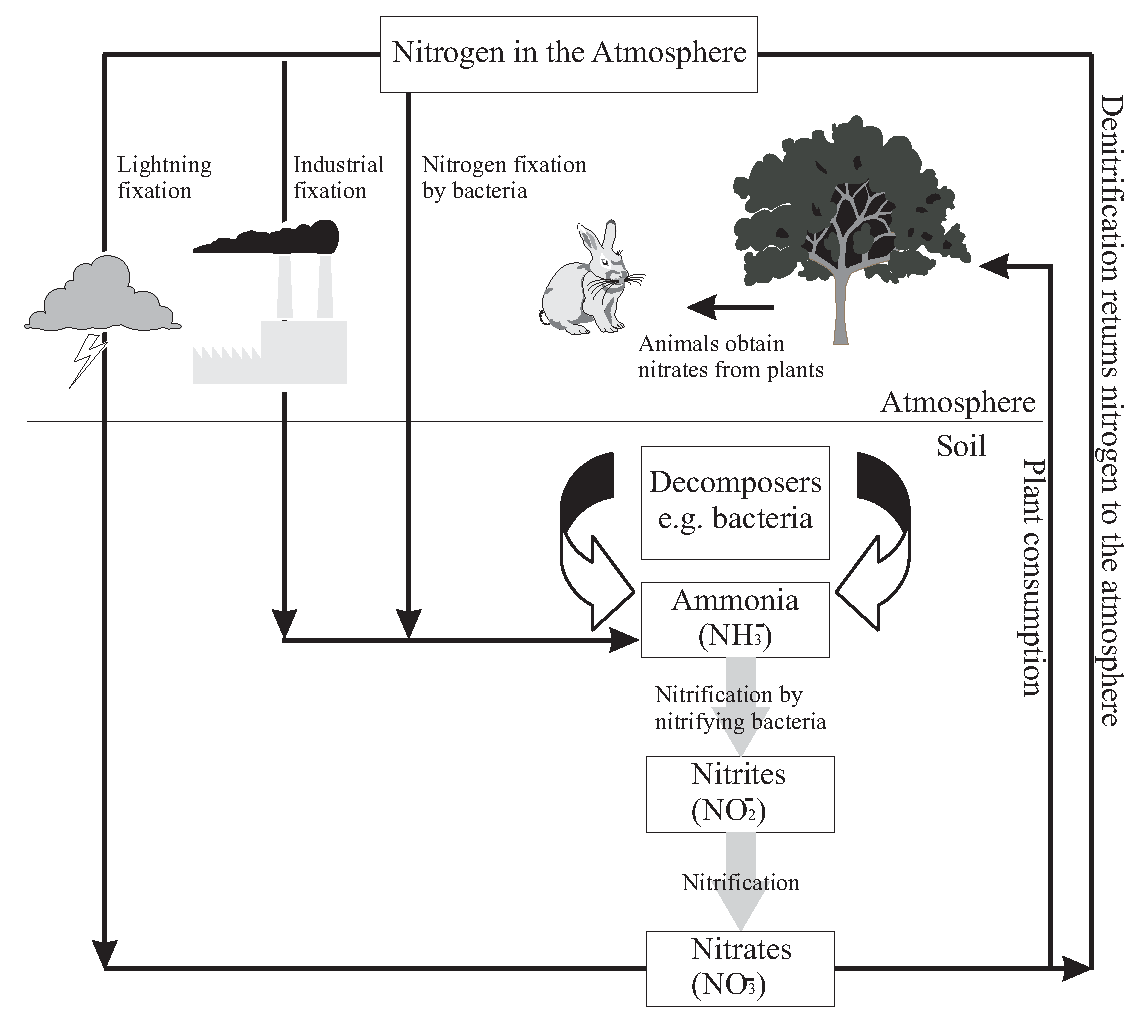
\includegraphics[width=13cm]{../NitrogenCycle.eps}
\end{center}
\caption{A simplified diagram of the nitrogen cycle}
\label{fig:global cycles:nitrogen cycle}
\end{figure}


% CHILD SECTION END 



% CHILD SECTION START 

\section{Nitrogen fixation}
\label{sec:global cycles: nitrogen fixation}

Nitrogen fixation is needed to change gaseous nitrogen into forms such as ammonia that are more useful to living organisms. Some fixation occurs in lightning strikes and in industrial processes, but most fixation is done by different types of bacteria living either in the soil or in parts of the plants. 

\begin{enumerate}
\item{\textbf{Biological fixation}

Some bacteria are able to fix nitrogen. They use an enzyme called \textit{nitrogenase} to combine gaseous nitrogen with hydrogen to form ammonia. The bacteria then use some of this ammonia to produce their own organic compounds, while what is left of the ammonia becomes available in the soil. \\

Some of these bacteria are free-living, in other words they live in the soil. Others live in the root nodules of legumes (e.g. soy, peas and beans). Here they form a mutualistic relationship with the plant. The bacteria get carbohydrates (food) from the plant and, in exchange, produce ammonia which can be converted into nitrogen compounds that are essential for the survival of the plant. In nutrient-poor soils, planting lots of legumes can help to enrich the soil with nitrogen compounds.

A simplified equation for biological nitrogen fixation is:
\begin{center}
\rm${N_{2} + 8H^{+} + 8e^{-} \rightarrow 2NH_{3} + H_{2}}$
\end{center}

In this equation the 8e$^{-}$ means 8 electrons.

Energy is used in the process, but this is not shown in the above equation.\\

Another important source of ammonia in the soil is \textbf{decomposition}. When animals and plants die, the nitrogen compounds that were present in them are broken down and converted into ammonia. This process is carried out by decomposition bacteria and fungi in the soil.
}

\item{\textbf{Industrial nitrogen fixation}

In the Haber-Bosch process, nitrogen (N$_{2}$) is converted together with hydrogen gas (H$_{2}$) into ammonia (NH$_{3}$) fertiliser. This is an artificial process.}
 
\item{\textbf{Lightning}

In the atmosphere, lightning and photons are important in the reaction between nitrogen (N$_{2}$) and oxygen (O$_{2}$) to form nitric oxide (NO) and then nitrates.}

\end{enumerate}

\begin{IFact}{It is interesting to note that by cultivating legumes, using the Haber-Bosch process to manufacture chemical fertilisers and increasing pollution from vehicles and industry, humans have more than doubled the amount of nitrogen that would normally be changed from nitrogen gas into a biologically useful form. This has serious environmental consequences.}
\end{IFact}



% CHILD SECTION END 



% CHILD SECTION START 

\section{Nitrification}
\label{sec:global cycles:nitrification}

Nitrification involves two biological oxidation reactions: firstly, the oxidation of ammonia with oxygen to form nitrite (NO$_{2}^{-}$) and secondly the oxidation of these nitrites into nitrates. 

\begin{center}
\begin{enumerate}
\item{\rm${NH_{3} + O_{2} \rightarrow NO_{2}^{-} + 3H^{+} + 2e^{-}}$ (production of \textit{nitrites})}

\item{\rm${NO_{2}^{-} + H_{2}O \rightarrow NO_{3}^{-} + 2H^{+} + 2e^{-}}$ (production of \textit{nitrates})}
\end{enumerate}
\end{center}

Nitrification is an important step in the nitrogen cycle in soil because it converts the ammonia (from the nitrogen fixing part of the cycle) into nitrates, which are easily absorbed by the roots of plants. This absorption of nitrates by plants is called \textbf{assimilation}. Once the nitrates have been assimilated by the plants, they become part of the plants' proteins. These plant proteins are then available to be eaten by animals. In other words, animals (including humans) obtain their own nitrogen by feeding on plants. Nitrification is performed by bacteria in the soil, called \textit{nitrifying bacteria}. \\

\Activity{Case Study}{Nitrates in drinking water\\}{

\textit{Read the information below and then carry out your own research to help you answer the questions that follow.}\\

The negatively charged nitrate ion is not held onto soil particles and so can be easily washed out of the soil. This is called \textbf{leaching}. In this way, valuable nitrogen can be lost from the soil, reducing the soil's fertility. The nitrates can then accumulate in groundwater, and eventually in drinking water. There are strict regulations that control how much nitrate can be present in drinking water, because nitrates can be reduced to highly reactive nitrites by microorganisms in the gut. Nitrites are absorbed from the gut and bind to haemoglobin (the pigment in blood that helps to transport oxygen around the body). This reduces the ability of the haemoglobin to carry oxygen. In young babies this can lead to respiratory distress, a condition known as "blue baby syndrome".\\

\begin{enumerate}
\item{How is nitrate concentration in water measured?}
\item{What concentration of nitrates in drinking water is considered acceptable? You can use drinking water standards for any part of the world, if you can't find any for South Africa.}
\item{What is 'blue baby syndrome' and what are the symptoms of the disease?}
\end{enumerate}

}


% CHILD SECTION END 



% CHILD SECTION START 

\section{Denitrification}
\label{sec:global cycles:denitrification}

Denitrification is the process of reducing nitrate and nitrite into gaseous nitrogen. The process is carried out by \textit{denitrification bacteria}. The nitrogen that is produced is returned to the atmosphere to complete the nitrogen cycle.\\

The equation for the reaction is:
\begin{center}
\rm${2NO_{3}^{-} + 10e^{-} + 12H^{+} \rightarrow N_{2} + 6H_{2}O}$
\end{center} 




% CHILD SECTION END 



% CHILD SECTION START 

\section{Human Influences on the Nitrogen Cycle}
\label{sec:global cycles:human influences}

Humans have contributed significantly to the nitrogen cycle in a number of ways. 

\begin{itemize}
\item{Both \textbf{artificial fertilisation} and the planting of \textbf{nitrogen fixing crops}, increase the amount of nitrogen in the soil. In some ways this has positive effects because it increases the fertility of the soil, and means that agricultural productivity is high. On the other hand, however, if there is too much nitrogen in the soil, it can run off into nearby water courses such as rivers, or can become part of the groundwater supply as we mentioned earlier. Increased nitrogen in rivers and dams can lead to a problem called \textbf{eutrophication}. Eutrophication is the contamination of a water system with excess nurtrients, which stimulates excessive algae growth at the expense of other parts of the ecosystem.  This occurs as eutrophication reduces oxygen levels in the water. Sometimes this can cause certain plant species to be favoured over the others and one species may 'take over' the ecosystem, resulting in a decrease in plant diversity. This is called a 'bloom'. Eutrophication also affects water quality. When the plants die and decompose, large amounts of oxygen are used up and this can cause other animals in the water to die.

\Activity{Case Study}{Fertiliser use in South Africa\\}{

Refer to the data table below, which shows the average fertiliser use (in kilograms per hectare or kg/ha) over a number of years for South Africa and the world. Then answer the questions that follow:\\

\begin{center}
\begin{tabular}{|l|p{0.7cm}|p{0.7cm}|p{0.7cm}|p{0.7cm}|p{0.7cm}|p{0.7cm}|p{0.7cm}|p{0.7cm}|p{0.7cm}|}\hline
 & \textbf{1965} & \textbf{1970} & \textbf{1975} & \textbf{1980} & \textbf{1985} & \textbf{1990} & \textbf{1995} & \textbf{2000} & \textbf{2002}\\\hline
\textbf{SA} & 27.9 & 42.2 & 57.7 & 80.3 & 66.6 & 54.9 & 48.5 & 47.1 & 61.4 \\\hline
\textbf{World} & 34.0 & 48.9 & 63.9 & 80.6 & 86.7 & 90.9 & 84.9 & 88.2 & 91.9 \\\hline
\end{tabular}
\end{center}

\begin{enumerate}
\item{On the same set of axes, draw two line graphs to show how fertiliser use has changed in SA and the world between 1965 and 2002.}
\item{Describe the trend you see for...
	\begin{enumerate}
	\item{the world}
	\item{South Africa}
	\end{enumerate}
}
\item{Suggest a reason why the world's fertiliser use has changed in this way over time.}
\item{Do you see the same pattern for South Africa?}
\item{Try to suggest a reason for the differences you see in the fertiliser use data for South Africa.}
\item{One of the problems with increased fertiliser use is that there is a greater chance of nutrient runoff into rivers and dams, and therefore a greater danger of eutrophication. In groups of 5-6, discuss the following questions:
	\begin{enumerate}
	\item{What could farmers do to try to reduce the risk of nutrient runoff from fields into water systems? Try to think of at least 3 different strategies that they could use.}
	\item{Imagine you are going to give a presentation on eutrophication to a group of farmers who know nothing about it. How will you educate them about the dangers? How will you convince them that it is in their interests to change their farming practices? Present your ideas to the class.}
	\end{enumerate}
} 
\end{enumerate}

}
}

\item{\textbf{Atmospheric pollution} is another problem. The main culprits are nitrous oxide (N$_{2}$O), nitric oxide (NO) and nitrogen dioxide (NO$_{2}$). Most of these gases result either from emissions from agricultural soils (and particularly artificial fertilisers), or from the combustion of fossil fuels in industry or motor vehicles. The combustion (burning) of nitrogen-bearing fuels such as coal and oil releases this nitrogen as NO$_{2}$ or NO gases. Both NO$_{2}$ and NO can combine with water droplets in the atmosphere to form \textbf{acid rain}. Furthermore, both NO and NO$_{2}$ contribute to the depletion of the ozone layer and some are \textbf{greenhouse gases}. In high concentrations these gases can contribute towards \textbf{global warming}.}


\end{itemize}



% CHILD SECTION END 



% CHILD SECTION START 

\section{The industrial fixation of nitrogen}
\label{sec:global cycles:industrial fixation}

A number of industrial processes are able to fix nitrogen into different compounds and then convert these compounds into fertilisers. In the descriptions below, you will see how atmospheric nitrogen is fixed to produce ammonia, how ammonia is then reacted with oxygen to form nitric acid and how nitric acid and ammonia are then used to produce the fertiliser, ammonium nitrate.

\begin{itemize} 
\item{\textbf{Preparation of ammonia (NH$_{3}$)}

The industrial preparation of ammonia is known as the \textbf{Haber-Bosch process}. At a high pressure and a temperature of approximately 500$^{0}$C, and in the presence of a suitable catalyst (usually iron), nitrogen and hydrogen react according to the following equation:
\begin{center}
\rm${N_{2} + 3H_{2} \rightarrow 2NH_{3}}$
\end{center}

Ammonia is used in the preparation of artficial fertilisers such as (NH$_{4}$)$_{2}$SO$_{4}$ and is also used in cleaning agents and cooling installations.
}

\begin{IFact}{
Fritz Haber and Carl Bosch were the two men responsible for developing the Haber-Bosch process. In 1918, Haber was awarded the Nobel Prize in Chemistry for his work. The Haber-Bosch process was a milestone in industrial chemistry because it meant that nitrogenous fertilisers were cheaper and much more easily available. At the time, this was very important in providing food for the growing human population.\\

Haber also played a major role in the development of chemical warfare in World War I. Part of this work included the development of gas masks with absorbent filters. He also led the teams that developed chlorine gas and other deadly gases for use in trench warfare. His wife, Clara Immerwahr, also a chemist, opposed his work on poison gas and committed suicide with his service weapon in their garden. During the 1920s, scientists working at his institute also developed the cyanide gas formulation Zyklon B, which was used as an insecticide and also later, after he left the programme, in the Nazi extermination camps. \\

Haber was Jewish by birth, but converted from Judaism in order to be more accepted in Germany. Despite this, he was forced to leave the country in 1933 because he was Jewish 'by definition' (his mother was Jewish). He died in 1934 at the age of 65. Many members of his extended family died in the Nazi concentration camps, possibly gassed by Zyklon B.
}
\end{IFact}

\item{\textbf{Preparation of nitric acid (HNO$_{3}$)}

Nitric acid is used to prepare fertilisers and explosives. The industrial preparation of nitric acid is known as the \textbf{Ostwald process}. The Ostwald process involves the conversion of ammonia into nitric acid in various stages:\\

Firstly, ammonia is heated with oxygen in the presence of a platinum catalyst to form nitric oxide and water.

\begin{center}
\rm${4NH_{3}(g) + 5O_{2}(g) \rightarrow 4NO(g) + 6H_{2}O(g)}$
\end{center}

Secondly, nitric oxide reacts with oxygen to form nitrogen dioxide. This gas is then readily absorbed by the water to produce nitric acid. A portion of nitrogen dioxide is reduced back to nitric oxide.

\begin{center}
\rm${2NO(g) + O_{2}(g) \rightarrow 2NO_{2}(g)}$\\

\rm${3NO_{2}(g) + H_{2}O(l) \rightarrow 2HNO_{3}(aq) + NO(g)}$
\end{center}

The NO is recycled, and the acid is concentrated to the required strength by a process called \textit{distillation}.
}

\item{\textbf{Preparation of ammonium nitrate}

Ammonium nitrate is used as a fertiliser, as an explosive and also in the preparation of 'laughing gas' which is used as an anaesthetic. Ammonium nitrate is prepared by reacting ammonia with nitric acid:

\begin{center}
\rm${NH_{3} + HNO_{3} \rightarrow NH_{4}NO_{3}}$
\end{center}
}
\end{itemize}

\Activity{Debate}{Fertiliser use\\}{

Divide the class into two groups to debate the following topic:\\

\begin{center}
\textit{Increasing the use of artificial fertilisers is the best solution to meet the growing food needs of the world's human population.\\}
\end{center}

One group should take the position of \textit{agreeing} with the statement, and the other should \textit{disagree}. In your groups, discuss reasons why you have the opinion that you do, and record some notes of your discussion. Your teacher will then explain to you how to proceed with the debate.
}

\section{Summary}

\begin{itemize}
\item{\textbf{Nitrogen} is essential for life on earth, since it forms part of \textbf{amino acids}, \textbf{proteins} and \textbf{nucleic acids}.}
\item{The \textbf{atmosphere} is composed mostly of nitrogen gas, but the gas is \textbf{inert}, meaning that it is not available to living organisms in its gaseous form.}
\item{The \textbf{nitrogen cycle} describes how nitrogen and nitrogen-containing compounds are changed into different forms in nature.}
\item{The nitrogen cycle consists of three major processes: \textbf{nitrogen fixation}, \textbf{nitrification} and \textbf{denitrification}.}
\item{\textbf{Nitrogen fixation} is the conversion of atmospheric nitrogen into compounds such as ammonia, that are more easily used.}
\item{Nitrogen can be fixed \textbf{biologically} through the actions of \textbf{bacteria}, \textbf{industrially} through the \textbf{Haber-Bosch process} or by \textbf{lightning}.}
\item{\textbf{Nitrification} converts ammonia into \textbf{nitrites} and \textbf{nitrates}, which can be easily \textbf{assimilated} by plants.}
\item{\textbf{Denitrification} converts nitrites and nitrates back into gaseous nitrogen to complete the nitrogen cycle.}
\item{\textbf{Humans} have had a number of \textbf{impacts} on the nitrogen cycle. The production of \textbf{artificial fertilisers} for example, means that there is a greater chance of runoff into water systems. In some cases, \textbf{eutrophication} may occur.}
\item{\textbf{Eutrophication} is the contamination of a water system with excess nurtrients, which stimulates excessive algae growth at the expense of other parts of the ecosystem.  This occurs as eutrophication reduces oxygen levels in the water.}
\item{Many nitrogen gases such as NO, N$_{2}$O and NO$_{2}$ are released by agricultural soils and artificial fertilisers. These gases may combine with water vapour in the atmosphere and result in \textbf{acid rain}. Some of these gases are also greenhouse gases and may contribute towards \textbf{global warming}.}
\item{A number of \textbf{industrial processes} are used to produce \textbf{articifical fertilisers}.}
\item{The \textbf{Haber-Bosch process} converts atmsopheric nitrogen into \textbf{ammonia}.}
\item{The \textbf{Ostwald process} reacts ammonia with oxygen to produce \textbf{nitric acid}, which is used in the preparation of fertilisers and explosives.}
\item{If ammonia and nitric acid react, the product is \textbf{ammonium nitrate}, which is used as a fertiliser and as an explosive.}
\end{itemize}

\Exercise{Summary Exercise\\}{
\begin{enumerate}
\item{Look at the diagram and the descriptions of the nitrogen cycle earlier in the chapter:}
	\begin{enumerate}
	\item{Would you describe the changes that take place in the nitrogen cycle as \textit{chemical} or \textit{physical} changes? Explain your answer.}
	\item{Are the changes that take place in the water cycle \textit{physical} or \textit{chemical} changes? Explain your answer.}
	\end{enumerate}
\item{Explain what is meant by each of the following terms:}
	\begin{enumerate}
	\item{nitrogen fixing}
	\item{fertiliser}
	\item{eutrophication}
	\end{enumerate}
\item{Explain why the fixing of atmospheric nitrogen is so important for the survival of life on earth.}
\item{Refer to the diagram below and then answer the questions that follow:

\begin{center}
\begin{pspicture}(-4,-1)(4,4)
%\psgrid[gridcolor=lightgray]
\psframe(-5,2)(-3,3)
\psline[linewidth=1pt,arrows=->](-2.8,2.5)(-1.8,2.5)

\psframe(-1.6,2)(0.4,3)
\psline[linewidth=1pt,arrows=->](0.6,2.5)(1.6,2.5)
\psframe(1.8,2)(3.8,3)
\psline[linewidth=1pt](2.3,1.8)(2.3,0.8)
\psline[linewidth=1pt](2.3,0.8)(-4,0.8)
\psline[linewidth=1pt,arrows=->](-4,0.8)(-4,1.8)

\rput(-4,2.5){N$_{2}$}
\rput(-2.3,2.7){(1)}
\rput(-0.6,2.5){(2)}
\rput(1.1,2.7){(3)}
\rput(2.8,2.5){(4)}
\rput(-0.4,0.5){(5)}

\end{pspicture}
\end{center}


	\begin{enumerate}
	\item{Explain the role of \textit{decomposers} in the nitrogen cycle. }
	\item{If the process taking place at (3) is \textit{nitrification}, then label the processes at (1) and (5).}
	\item{Identify the nitrogen products at (2) and (4).}
	\item{On the diagram, indicate the type of \textit{bacteria} that are involved in each stage of the nitrogen cycle.}
	\item{In industry, what process is used to produce the compound at 2?}
	\item{Does the diagram above show a 'cycle'? Explain your answer.}
	\end{enumerate}
}
\item{NO and NO$_{2}$ are both nitrogen compounds:
	\begin{enumerate}
	\item{Explain how each of these compounds is formed?}
	\item{What effect does each of these compounds have in the environment?}
	\end{enumerate}
}
\item{There are a number of arguments both 'for' and 'against' the use of artificial fertilisers. Draw a table to summarise the advantages and disadvantages of their use.}
\end{enumerate}
}


% CHILD SECTION END 



% CHILD SECTION END 



% CHILD SECTION START 

\chapter{The Hydrosphere - Grade 10}
\label{chap:hydrosphere}


% CHILD SECTION START 

\section{Introduction}


As far as we know, the Earth we live on is the only planet that is able to support life. Among other things, Earth is just the right distance from the sun to have temperatures that are suitable for life to exist. Also, the Earth's atmosphere has exactly the right type of gases in the right amounts for life to survive. Our planet also has \textbf{water} on its surface, which is something very unique. In fact, Earth is often called the 'Blue Planet' because most of it is covered in water. This water is made up of \textit{freshwater} in rivers and lakes, the \textit{saltwater} of the oceans and estuaries, \textit{groundwater} and \textit{water vapour}. Together, all these water bodies are called the \textbf{hydrosphere}.


% CHILD SECTION END 



% CHILD SECTION START 

\section{Interactions of the hydrosphere}

It is important to realise that the hydrosphere interacts with other global systems, including the \textit{atmosphere}, \textit{lithosphere} and \textit{biosphere}.

\begin{itemize}
\item{\textit{Atmosphere}

When water is heated (e.g. by energy from the sun), it evaporates and forms water vapour. When water vapour cools again, it condenses to form liquid water which eventually returns to the surface by precipitation e.g. rain or snow. This cycle of water moving through the atmosphere, and the energy changes that accompany it, is what drives weather patterns on earth.
}
\item{\textit{Lithosphere}

In the lithosphere (the ocean and continental crust at the Earth's surface), water is an important \textit{weathering} agent, which means that it helps to break rock down into rock fragments and then soil. These fragments may then be transported by water to another place, where they are deposited. This is called \textit{erosion}. These two process i.e. weathering and erosion, help to shape the earth's surface. You can see this for example in rivers. In the upper streams, rocks are eroded and sediments are transported down the river and deposited on the wide flood plains lower down. On a bigger scale, river valleys in mountains have been carved out by the action of water, and cliffs and caves on rocky beach coastlines, are also the result of weathering and erosion by water.
}
\item{\textit{Biosphere}

In the biosphere, land plants absorb water through their roots and then transport this through their vascular (transport) system to stems and leaves. This water is needed in \textit{photosynthesis}, the food production process in plants. Transpiration (evaporation of water from the leaf surface) then returns water back to the atmosphere.
}
\end{itemize} 


% CHILD SECTION END 



% CHILD SECTION START 

\section{Exploring the Hydrosphere}
\label{sec:hydro:exploring}

The large amount of water on our planet is something quite unique. In fact, about 71\% of the earth is covered by water. Of this, almost 97\% is found in the oceans as saltwater, about 2.2\% occurs as a solid in ice sheets, while the remaining amount (less than 1\%) is available as freshwater. So from a human perspective, despite the vast amount of water on the planet, only a very small amount is actually available for human consumption (e.g. drinking water). Before we go on to look more closely at the chemistry of the hydrosphere, we are going to spend some time exploring a part of the hydrosphere, in order to start appreciating what a complex and beautiful part of the world it is.

\Activity{Investigation}{Investigating the hydrosphere\\}{

\begin{enumerate}

\item{
\textbf{Choosing a study site:\\}

For this exercise, you can choose any part of the hydrosphere that you would like to explore. This may be a rock pool, a lake, river, wetland or even just a small pond. The guidelines below will apply best to a river investigation, but you can ask similar questions and gather similar data in other areas. When choosing your study site, consider how accessible it is (how easy is it to get to?) and the problems you may experience (e.g. tides, rain).\\
}

\item{
\textbf{Collecting data:\\}

Your teacher will provide you with the equipment you need to collect the following data. You should have at least one study site where you will collect data, but you might decide to have more if you want to compare your results in different areas. This works best in a river, where you can choose sites down its length. \\

\begin{enumerate}
\item{\textit{Chemical data}

Measure and record data such as temperature, pH, conductivity and dissolved oxygen at each of your sites. You may not know exactly what these measurements mean right now, but it will become clearer later in the chapter.}

\item{\textit{Hydrological data}

Measure the water velocity of the river and observe how the volume of water in the river changes as you move down its length. You can also collect a water sample in a clear bottle, hold it to the light and see whether the water is clear  or whether it has particles in it.}

\item{\textit{Biological data}

What types of animals and plants are found in or near this part of the hydrosphere? Are they specially adapted to their environment?\\}
\end{enumerate}

Record your data in a table like the one shown below:

\begin{center}
\begin{tabular}{|l|c|c|c|}\hline
 & \textbf{Site 1} & \textbf{Site 2} & \textbf{Site 3}\\\hline
\textbf{Temperature} & & & \\\hline
\textbf{pH} & & & \\\hline
\textbf{Conductivity} & & & \\\hline
\textbf{Dissolved oxygen} & & & \\\hline
\textbf{Animals and plants} & & & \\\hline
\end{tabular}
\end{center}
}

\item{
\textbf{Interpreting the data:\\}

Once you have collected and recorded your data, think about the following questions:

\begin{itemize}
\item{How does the data you have collected vary at different sites?}
\item{Can you explain these differences?}
\item{What effect do you think \textit{temperature}, \textit{dissolved oxygen} and \textit{pH} have on animals and plants that are living in the hydrosphere?}
\item{Water is seldom 'pure'. It usually has lots of things dissolved (e.g. Mg, Ca and NO$_{3}^{-}$ ions) or suspended (e.g. soil particles, debris) in it. Where do these substances come from?}
 
\item{Are there any human activities near this part of the hydrosphere? What effect could these activities have on the hydrosphere?}
\end{itemize}
}
\end{enumerate}
}



% CHILD SECTION END 



% CHILD SECTION START 

\section{The Importance of the Hydrosphere}
\label{sec:hydro:importance}

It is so easy sometimes to take our hydrosphere for granted, and we seldom take the time to really think about the role that this part of the planet plays in keeping us alive. Below are just some of the very important functions of water in the hydrosphere:

\begin{itemize}
\item{\textit{Water is a part of living cells}

Each cell in a living organism is made up of almost 75\% water, and this allows the cell to function normally. In fact, most of the chemical reactions that occur in life, involve substances that are dissolved in water. Without water, cells would not be able to carry out their normal functions, and life could not exist.}

\item{\textit{Water provides a habitat}

The hydrosphere provides an important place for many animals and plants to live. Many gases (e.g. CO$_{2}$, O$_{2}$), nutrients e.g. nitrate (NO$_{3}^{-}$), nitrite (NO$_{2}^{-}$) and ammonium (NH$_{4}^{+}$) ions, as well as other ions (e.g. Ca$^{2+}$ and Mg$^{2+}$) are dissolved in water. The presence of these substances is critical for life to exist in water.}
\item{\textit{Regulating climate} 

%You may remember from chapter \ref{chap:globalcycles} that 
One of water's unique characteristics is its high \textit{specific heat}. This means that water takes a long time to heat up, and also a long time to cool down. This is important in helping to regulate temperatures on earth so that they stay within a range that is acceptable for life to exist. \textit{Ocean currents} also help to disperse heat. }
\item{\textit{Human needs}

Humans use water in a number of ways. Drinking water is obviously very important, but water is also used domestically (e.g. washing and cleaning) and in industry. Water can also be used to generate electricity through hydropower.}
\end{itemize}

These are just a few of the very important functions that water plays on our planet. Many of the functions of water relate to its chemistry and to the way in which it is able to dissolve substances in it.



% CHILD SECTION END 



% CHILD SECTION START 

\section{Ions in aqueous solution}
\label{sec:hydro:ions in solution}

As we mentioned earlier, water is seldom pure. Because of the structure of the water molecule, it is able to dissolve substances in it. This is very important because if water wasn't able to do this, life would not be able to survive. In rivers and the oceans for example, dissolved oxygen means that organisms (such as fish) are still able to respire (breathe). For plants, dissolved nutrients are also available. In the human body, water is able to carry dissolved substances from one part of the body to another.\\

Many of the substances that dissolve are \textit{ionic}, and when they dissolve they form ions in solution. We are going to look at how water is able to dissolve ionic compounds, and how these ions maintain a balance in the human body, how they affect water hardness, and how specific ions determine the pH of solutions. 

\subsection{Dissociation in water}

Water is a \textbf{polar molecule} (figure \ref{fig:hydrosphere:water}). This means that one part of the molecule has a slightly positive charge and the other part has a slightly negative charge.\\

\begin{figure}[!h]
\begin{center}
\begin{pspicture}(-2,-1)(2,1.4)
%\psgrid[gridcolor=lightgray]
\psellipse(0,0)(2,1)
\rput(-1.5,0){\textbf{$\delta^{+}$}}
\rput(1.5,0){\textbf{$\delta^{-}$}}
\rput(0,0){\textbf{H$_{2}$O}}
\end{pspicture}
\end{center}
\caption{Water is a polar molecule}
\label{fig:hydrosphere:water}
\end{figure}

It is the polar nature of water that allows ionic compounds to dissolve in it. In the case of sodium chloride (NaCl) for example, the positive sodium ions (Na$^{+}$) will be attracted to the negative pole of the water molecule, while the negative chloride ions (Cl$^{-}$) will be attracted to the positive pole of the water molecule. In the process, the ionic bonds between the sodium and chloride ions are weakened and the water molecules are able to work their way between the individual ions, surrounding them and slowly dissolving the compound. This process is called \textbf{dissociation}. A simplified representation of this is shown in figure \ref{fig:hydrosphere:ions dissolving}. \\

\Definition{Dissociation}{Dissociation in chemistry and biochemistry is a general process in which ionic compounds separate or split into smaller molecules or ions, usually in a reversible manner. }

\begin{figure}[!h]
\begin{center}
\begin{pspicture}(-4,-4)(4,4)
%\psgrid[gridcolor=lightgray]
\psellipse(0,0)(0.5,0.5)
\psellipse(1.5,0)(1,0.5)
\psellipse(0,-1.5)(0.5,1)
\psellipse(-1.5,0)(1,0.5)
\psellipse(0,1.5)(0.5,1)
\psellipse(-3,0)(0.5,0.5)
\psellipse(0,3)(0.5,0.5)
\psellipse(3,0)(0.5,0.5)
\psellipse(0,-3)(0.5,0.5)

\rput(0,0){\textbf{$Na^{+}$}}
\rput(3,0){\textbf{$Cl^{-}$}}
\rput(-3,0){\textbf{$Cl^{-}$}}
\rput(0,3){\textbf{$Cl^{-}$}}
\rput(0,-3){\textbf{$Cl^{-}$}}

\rput(1.5,0){\textbf{$H_{2}O$}}
\rput(-1.5,0){\textbf{$H_{2}O$}}
\rput(0,1.5){\textbf{$H_{2}O$}}
\rput(0,-1.5){\textbf{$H_{2}O$}}

\rput(0.8,0){$\delta^{-}$}
\rput(-0.8,0){$\delta^{-}$}
\rput(0,0.8){$\delta^{-}$}
\rput(0,-0.8){$\delta^{-}$}

\rput(2.2,0){$\delta^{+}$}
\rput(-2.2,0){$\delta^{+}$}
\rput(0,2.2){$\delta^{+}$}
\rput(0,-2.2){$\delta^{+}$}
\end{pspicture}
\caption{Sodium chloride dissolves in water}
\label{fig:hydrosphere:ions dissolving}
\end{center}
\end{figure}

The dissolution of sodium chloride can be represented by the following equation:

\begin{equation*}
NaCl(s) \rightarrow Na^{+}(aq) + Cl^{-}(aq) 
\end{equation*}

The symbols \textbf{s} (solid), \textbf{l} (liquid), \textbf{g} (gas) and \textbf{aq} (material is dissolved in water) are written after the chemical formula to show the state or phase of the material. The dissolution of potassium sulfate into potassium and sulfate ions is shown below as another example:

\begin{equation*} 
K_{2}SO_{4}(s) \rightarrow 2K^{+}(aq) + SO_{4}^{2-}(aq)
\end{equation*}

Remember that \textbf{molecular} substances (e.g. covalent compounds) may also dissolve, but most will not form ions. One example is sugar.

\begin{equation*}
C_{6}H_{12}O_{6}(s) \rightleftharpoons C_{6}H_{12}O_{6}(aq)
\end{equation*}

There are exceptions to this and some molecular substances \textit{will} form ions when they dissolve. Hydrogen chloride for example can ionise to form hydrogen and chloride ions.

\begin{equation*}
HCl (g) \rightarrow H^{+} (aq) + Cl^{-} (aq)
\end{equation*}



\begin{IFact}{The ability of ionic compounds to dissolve in water is extremely important in the human body! The body is made up of \textit{cells}, each of which is surrounded by a \textit{membrane}. Dissolved ions are found inside and outside of body cells, in different concentrations. Some of these ions are positive (e.g. Mg$^{2+}$) and some are negative (e.g. Cl$^{-}$). If there is a difference in the charge that is inside and outside the cell, then there is a \textit{potential difference} across the cell membrane. This is called the \textbf{membrane potential} of the cell. The membrane potential acts like a battery and affects the movement of all charged substances across the membrane.  Membrane potentials play a role in muscle functioning, digestion, excretion and in maintaining blood pH, to name just a few. The movement of ions across the membrane can also be converted into an electric signal that can be transferred along \textit{neurons} (nerve cells), which control body processes. If ionic substances were not able to dissociate in water, then none of these processes would be possible! It is also important to realise that our bodies can \textit{lose} ions such as Na$^{+}$, K$^{+}$, Ca$^{2+}$, Mg$^{2+}$, and Cl$^{-}$, for example when we sweat during exercise. Sports drinks such as Lucozade and Powerade are designed to replace these lost ions so that the body's normal functioning is not affected.}
\end{IFact}

\Exercise{Ions in solution\\}{

\begin{enumerate}
\item{For each of the following, say whether the substance is ionic or molecular.}
	\begin{enumerate}
	\item{potassium nitrate (KNO$_{3}$)}
	\item{ethanol (C$_{2}$H$_{5}$OH)}
	\item{sucrose (a type of sugar) (C$_{12}$H$_{22}$O$_{11}$}
	\item{sodium bromide (NaBr)}
	\end{enumerate}

\item{Write a balanced equation to show how each of the following ionic compounds dissociate in water.}
	\begin{enumerate}
	\item{sodium sulphate (Na$_{2}$SO$_{4}$)}
	\item{potassium bromide (KBr)}
	\item{potassium permanganate (KMNO$_{4}$)}
	\item{sodium phosphate (Na$_{3}$PO$_{4}$)}
	\end{enumerate}
\end{enumerate}
}

\subsection{Ions and water hardness}

\Definition{Water hardness}{Water hardness is a measure of the mineral content of water. Minerals are substances such as calcite, quartz and mica that occur naturally as a result of geological processes.}

\textbf{Hard water} is water that has a high mineral content. Water that has a low mineral content is known as \textbf{soft water}. If water has a high mineral content, it usually contains high levels of metal ions, mainly calcium (Ca) and magnesium (Mg). The calcium enters the water from either CaCO$_{3}$ (limestone or chalk) or from mineral deposits of CaSO$_{4}$. The main source of magnesium is a sedimentary rock called dolomite, CaMg(CO$_{3}$)$_{2}$. Hard water may also contain other metals as well as bicarbonates and sulphates. \\


\begin{IFact}{The simplest way to check whether water is hard or soft is to use the lather/froth test. If the water is very soft, soap will lather more easily when it is rubbed against the skin. With hard water this won't happen. Toothpaste will also not froth well in hard water.}
\end{IFact}

A \textbf{water softener} works on the principle of \textbf{ion exchange}. Hard water passes through a media bed, usually made of resin beads that are supersaturated with sodium. As the water passes through the beads, the hardness minerals (e.g. calcium and magnesium) attach themselves to the beads. The sodium that was originally on the beads is released into the water. When the resin becomes saturated with calcium and magnesium, it must be recharged. A salt solution is passed through the resin. The sodium replaces the calcium and magnesium, and these ions are released into the waste water and discharged. 

\subsection{The pH scale}

The concentration of specific ions in solution, affects whether the solution is acidic or basic. You will learn about acids and bases in Grade 11. Acids and bases can be described as substances that either increase or decrease the concentration of hydrogen (H$^{+}$ or H$_{3}$O$^{+}$) ions in a solution. An acid \textit{increases} the hydrogen ion concentration in a solution, while a base \textit{decreases} the hydrogen ion concentration. \textbf{pH} is used to measure whether a substance is acidic or basic (alkaline).

\Definition{pH}{pH is a measure of the acidity or alkalinity of a solution. The pH scale ranges from 0 to 14. Solutions with a pH less than seven are acidic, while those with a pH greater than seven are basic (alkaline). pH 7 is considered neutral.}

pH can be calculated using the following equation:

\begin{equation*}
pH = -log[H^{+}]
\end{equation*} 

or

\begin{equation*}
pH = -log[H_{3}O^{+}]
\end{equation*} 

The brackets in the above equation are used to show \textit{concentration} in mol.dm$^{-3}$. 

\begin{wex}{pH calculations}{Calculate the pH of a solution where the concentration of hydrogen ions is 1 $\times$ 10$^{-7}$ mol.dm$^{-3}$.\\}

{\westep{Determine the concentration of hydrogen ions in mol.dm$^{-3}$}

In this example, the concentration has been given and is 1 $\times$ 10$^{-7}$ mol.dm$^{-3}$\\
}
{\westep{Substitute this value into the pH equation and calculate the pH value}

pH = -log[H$^{+}$]

= -log(1 $\times$ 10$^{-7}$)

= 7
}
\end{wex}

\begin{wex}{pH calculations}{In a solution of ethanoic acid (or acetic acid), the following equilibrium is established:

\begin{center}
\rm${CH_{3}COOH(aq) + H_{2}O \rightleftharpoons CH_{3}COO^{-}(aq) + H_{3}O^{+}}$
\end{center}

The concentration of CH$_{3}$COO$^{-}$ ions is found to be 0.003 mol.dm$^{-3}$. Calculate the pH of the solution.\\
}

{\westep{Determine the concentration of hydrogen ions in the solution}

According to the balanced equation for this reaction, the mole ratio of CH$_{3}$COO$^{-}$ ions to H$_{3}$O$^{+}$ ions is the same, therefore the concentration of these two ions in the solution will also be the same. So, [H$_{3}$O$^{+}$] = 0.003 dm$^{-3}$.\\
}

{\westep{Substitute this value into the pH equation and calculate the pH value}

pH = -log[H$_{3}$O$^{+}$]

= -log(0.003)

= 2.52
}
\end{wex}

 
Understanding pH is very important. In living organisms, it is necessary to maintain a constant pH so that chemical reactions can occur under optimal conditions. 

\Tip{It may also be useful for calculations involving the pH scale, to know that the following equation can also be used:

\begin{center}
[H$_{3}$O$^{+}$][OH$^{-}$] = 1 $\times$ 10$^{-14}$
\end{center}
}

\begin{IFact}{A build up of acid in the human body can be very dangerous. \textbf{Lactic acidosis} is a condition caused by the buildup of lactic acid in the body. It leads to acidification of the blood (acidosis) and can make a person very ill. Some of the symptoms of lactic acidosis are deep and rapid breathing, vomiting, and abdominal pain. In the fight against HIV, lactic acidosis is a problem. One of the antiretrovirals (ARV's) that is used in anti-HIV treatment is Stavudine (also known as Zerit or d4T). One of the side effects of Stavudine is lactic acidosis, particularly in overweight women. If it is not treated quickly, it can result in death.
}
\end{IFact}

In agriculture, farmers need to know the pH of their soils so that they are able to plant the right kinds of crops. The pH of soils can vary depending on a number of factors such as rainwater, the kinds of rocks and materials from which the soil was formed and also human influences such as pollution and fertilisers. The pH of rain water can also vary and this too has an effect on agriculture, buildings, water courses, animals and plants. Rainwater is naturally acidic because carbon dioxide in the atmosphere combines with water to form carbonic acid. Unpolluted rainwater has a pH of approximately 5.6. However, human activities can alter the acidity of rain and this can cause serious problems such as acid rain.

\Exercise{Calculating pH\\}{

\begin{enumerate}

\item{Calculate the pH of each of the following solutions:}

	\begin{enumerate}
	\item{A 0.2 mol.dm$^{-3}$ KOH solution}
	\item{A 0.5 mol.dm$^{-3}$ HCl solution} 
	\end{enumerate}

\item{What is the concentration (in mol.dm$^{-3}$) of H$_{3}$O$^{+}$ ions in a NaOH solution which has a pH of 12?}

\item{The concentrations of hydronium (H$_{3}$O$^{+}$) and hydroxyl (OH$^{-}$) ions in a typical sample of seawater are 10$^{-8}$ mol.dm$^{-3}$ and 10$^{-6}$ mol.dm$^{-3}$ respectively.}
	\begin{enumerate}
	\item{Is the seawater acidic or basic?}
	\item{What is the pH of the seawater?}
	\item{Give a possible explanation for the pH of the seawater.}
	\end{enumerate}
(IEB Paper 2, 2002)
\end{enumerate}
}


\subsection{Acid rain}

The acidity of rainwater comes from the natural presence of three substances (CO$_{2}$, NO, and SO$_{2}$) in the lowest layer of the atmosphere. These gases are able to dissolve in water and therefore make rain more acidic than it would otherwise be. Of these gases, carbon dioxide (CO$_{2}$) has the highest concentration and therefore contributes the most to the natural acidity of rainwater. We will look at each of these gases in turn.

\Definition{Acid rain}{Acid rain refers to the deposition of acidic components in rain, snow and dew. Acid rain occurs when sulfur dioxide and nitrogen oxides are emitted into the atmosphere, undergo chemical transformations, and are absorbed by water droplets in clouds. The droplets then fall to earth as rain, snow, mist, dry dust, hail, or sleet. This increases the acidity of the soil, and affects the chemical balance of lakes and streams.}

\begin{enumerate}
\item{\textbf{Carbon dioxide}}

Carbon dioxide reacts with water in the atmosphere to form \textbf{carbonic acid} (H$_{2}$CO$_{3}$). 

\begin{equation*}
CO_{2} + H_{2}O \rightarrow H_{2}CO_{3}
\end{equation*}

The carbonic acid dissociates to form hydrogen and hydrogen carbonate ions. It is the presence of hydrogen ions that lowers the pH of the solution, making the rain acidic.

\begin{equation*}
H_{2}CO_{3} \rightarrow H^{+} + HCO_{3}^{-}
\end{equation*}

\item{\textbf{Nitric oxide}}

Nitric oxide (NO) also contributes to the natural acidity of rainwater and is formed during lightning storms when nitrogen and oxygen react. In air, NO is oxidised to form nitrogen dioxide (NO$_{2}$). It is the nitrogen dioxide which then reacts with water in the atmosphere to form \textbf{nitric acid} (HNO$_{3}$).

\begin{equation*}
3NO_{2} (g) + H_{2}O \rightarrow 2HNO_{3} (aq) + NO (g)
\end{equation*}

The nitric acid dissociates in water to produce hydrogen ions and nitrate ions. This again lowers the pH of the solution, making it acidic.

\begin{equation*}
HNO_{3} \rightarrow H^{+} + NO_{3}^{-}
\end{equation*}

\item{\textbf{Sulfur dioxide}}

Sulfur dioxide in the atmosphere first reacts with oxygen to form sulfur trioxide, before reacting with water to form \textbf{sulfuric acid}.

\begin{equation*}
2SO_{2} + O_{2} \rightarrow 2SO_{3} 
\end{equation*}

\begin{equation*}
SO_{3} + H_{2}O \rightarrow H_{2}SO_{4}
\end{equation*}

Sulfuric acid dissociates in a similar way to the previous reactions.

\begin{equation*}
H_{2}SO_{4} \rightarrow HSO_{4}^{-} + H^{+}
\end{equation*}

\end{enumerate}

Although these reactions do take place naturally, human activities can greatly increase the concentration of these gases in the atmosphere, so that rain becomes far more acidic than it would otherwise be. The burning of fossil fuels in industries, vehicles etc is one of the biggest culprits. If the acidity of the rain drops below 5, it is referred to as \textbf{acid rain}.\\

Acid rain can have a very damaging effect on the environment. In rivers, dams and lakes, increased acidity can mean that some species of animals and plants will not survive. Acid rain can also degrade soil minerals, producing metal ions that are washed into water systems. Some of these ions may be toxic e.g. Al$^{3+}$. From an economic perspective, altered soil pH can drastically affect agricultural productivity. \\

Acid rain can also affect buildings and monuments, many of which are made from marble and limestone. A chemical reaction takes place between CaCO$_{3}$ (limestone) and sulfuric acid to produce aqueous ions which can be easily washed away. The same reaction can occur in the lithosphere where limestone rocks are present e.g. limestone caves can be eroded by acidic rainwater.

\begin{equation*}
H_{2}SO_{4} + CaCO_{3} \rightarrow CaSO_{4}.H_{2}O + CO_{2}
\end{equation*}

\Activity{Investigation}{Acid rain\\}{

You are going to test the effect of 'acid rain' on a number of substances. \\

\textit{Materials needed:\\}

samples of chalk, marble, zinc, iron, lead, dilute sulfuric acid, test tubes, beaker, glass dropper\\

\textit{Method:\\}

\begin{enumerate}
\item{Place a small sample of each of the following substances in a separate test tube: chalk, marble, zinc, iron and lead}
\item{To each test tube, add a few drops of dilute sulfuric acid.}
\item{Observe what happens and record your results.\\}
\end{enumerate}

\textit{Discussion questions:}

\begin{itemize}
\item{In which of the test tubes did reactions take place? What happened to the sample substances?}
\item{What do your results tell you about the effect that acid rain could have on each of the following: buildings, soils, rocks and geology, water ecosystems?}
\item{What precautions could be taken to reduce the potential impact of acid rain?}
\end{itemize}
}



% CHILD SECTION END 



% CHILD SECTION START 

\section{Electrolytes, ionisation and conductivity}
\label{sec:hydrosphere:electrolytes}

\textbf{Conductivity} in aqueous solutions, is a measure of the ability of water to conduct an electric current. The more \textbf{ions} there are in the solution, the higher its conductivity.

\Definition{Conductivity}{Conductivity is a measure of a solution's ability to conduct an electric current.}

\subsection{Electrolytes}

An \textbf{electrolyte} is a material that \textit{increases} the conductivity of water when dissolved in it. Electrolytes can be further divided into \textbf{strong electrolytes} and \textbf{weak electrolytes}.

\Definition{Electrolyte}{An electrolyte is a substance that contains free ions and behaves as an electrically conductive medium. Because they generally consist of ions in solution, electrolytes are also known as ionic solutions.}

\begin{enumerate}
\item{\textbf{Strong electrolytes}

A strong electrolyte is a material that ionises completely when it is dissolved in water:

\begin{equation*}
AB (s,l,g) \rightarrow A^{+} (aq) + B^{-} (aq)
\end{equation*}

This is a \textbf{chemical change} because the original compound has been split into its component ions and bonds have been broken. In a strong electrolyte, we say that the \textit{extent of ionisation} is high. In other words, the original material dissociates completely so that there is a high concentration of ions in the solution. An example is a solution of potassium nitrate:

\begin{equation*}
KNO_{3} (s) \rightarrow K^{+} (aq) + NO_{3}^{-} (aq)
\end{equation*}
}

\item{\textbf{Weak electrolytes}

A weak electrolyte is a material that goes into solution and will be surrounded by water molecules when it is added to water. However, not \textit{all} of the molecules will dissociate into ions. The \textit{extent of ionisation} of a weak electrolyte is low and therefore the concentration of ions in the solution is also low.

\begin{equation*}
AB (s,l,g) \rightarrow AB (aq) \rightleftharpoons A^{+} (aq) + B^{-} (aq)
\end{equation*}

The following example shows that, in the final solution of a weak electrolyte, some of the original compound \textit{plus} some dissolved ions are present.

\begin{equation*}
C_{2}H_{3}O_{2}H (l) \rightarrow C_{2}H_{3}O_{2}H \rightleftharpoons C_{2}H_{3}O_{2}^{-} (aq) + H^{+} (aq)
\end{equation*}
}
\end{enumerate}

\subsection{Non-electrolytes}

A \textbf{non-electrolyte} is a material that does not increase the conductivity of water when dissolved in it. The substance goes into solution and becomes surrounded by water molecules, so that the molecules of the chemical become separated from each other. However, although the substance does dissolve, it is not changed in any way and no chemical bonds are broken. The change is a \textbf{physical change}. In the oxygen example below, the reaction is shown to be reversible because oxygen is only partially soluble in water and comes out of solution very easily.

\begin{equation*}
C_{2}H_{5}OH (l) \rightarrow C_{2}H_{5}OH (aq)
\end{equation*} 

\begin{equation*}
O_{2} (g) \rightleftharpoons O_{2} (aq)
\end{equation*}

\subsection{Factors that affect the conductivity of water}

The conductivity of water is therefore affected by the following factors:

\begin{itemize}

\item{The \textbf{type of substance} that dissolves in water  

Whether a material is a strong electrolyte (e.g. potassium nitrate, KNO$_{3}$), a weak electrolyte (e.g. acetate, C$_{2}$H$_{3}$O$_{2}$H) or a non-electrolyte (e.g. sugar, alcohol, oil) will affect the conductivity of water because the concentration of ions in solution will be different in each case.


}

\item{The \textbf{concentration of ions} in solution 

The higher the concentration of ions in solution, the higher its conductivity will be.
}

\item{\textbf{Temperature} 

The warmer the solution the higher the solubility of the material being dissolved, and therefore the higher the conductivity as well.
}
\end{itemize}

\Activity{Experiment}{Electrical conductivity \\}{

\Aim{

To investigate the electrical conductivities of different substances and solutions.}

\Apparatus{

solid salt (NaCl) crystals; different liquids such as distilled water, tap water, seawater, benzene and alcohol; solutions of salts e.g. NaCl, KBr; a solution of an acid (e.g. HCl) and a solution of a base (e.g. NaOH); torch cells; ammeter; conducting wire, crocodile clips and 2 carbon rods.}

\Method{

Set up the experiment by connecting the circuit as shown in the diagram below. In the diagram, 'X' represents the substance or solution that you will be testing. When you are using the solid crystals, the crocodile clips can be attached directly to each end of the crystal. When you are using solutions, two carbon rods are placed into the liquid, and the clips are attached to each of the rods. In each case, complete the circuit and allow the current to flow for about 30 seconds. Observe whether the ammeter shows a reading. 

\begin{center}
\begin{pspicture}(0,-0.6)(5,6.2)
\SpecialCoor
%\psgrid[gridcolor=lightgray]
\pnode(0,0){A}
\pnode(0,5){B}
\pnode(5,5){C}
\pnode(5,0){D}
\pnode(3.5,0){E}
\pnode(1.5,0){F}
\battery(B)(C){battery}
\psline(C)(D)
\psline[arrowsize=10pt,arrowinset=0,arrowlength=2.5]{->}(D)(E)
\psframe(1.5,-0.5)(3.5,0.5)
\uput[u](2.5,0.5){test substance}
\rput(2.5,0){X}
\psline(4,0)(4,-0.4)(4.6,-0.4)
\uput[r](4.6,-0.4){crocodile clip}
\psline[arrowsize=10pt,arrowinset=0,arrowlength=2.5]{<-}(F)(A)
\psellipse(0,2.5)(0.5,0.5)
\rput(0,2.5){\textbf{A}}
\psline(0,5)(0,3)
\psline(0,2)(0,0)
\rput(-1.5,2.5){Ammeter}
\end{pspicture}
\end{center}
}

\Results{

Record your observations in a table similar to the one below:

\begin{center}
\begin{tabular}{|c|c|}\hline
Test substance & Ammeter reading\\\hline
 & \\\hline
 & \\\hline
 & \\\hline
 & \\\hline
\end{tabular}
\end{center}


What do you notice? Can you explain these observations?\\

Remember that for electricity to flow, there needs to be a movement of charged particles e.g. ions. With the solid NaCl crystals, there was no flow of electricity recorded on the ammeter. Although the solid is made up of ions, they are held together very tightly within the crystal lattice, and therefore no current will flow. Distilled water, benzene and alcohol also don't conduct a current because they are \textit{covalent compounds} and therefore do not contain ions.\\

The ammeter should have recorded a current when the salt solutions and the acid and base solutions were connected in the circuit. In solution, salts \textit{dissociate} into their ions, so that these are free to move in the solution. Acids and bases behave in a similar way, and dissociate to form hydronium and oxonium ions. Look at the following examples:

\begin{center}

$\rm{KBr \rightarrow K^{+} + Br^{-}}$

$\rm{NaCl \rightarrow Na^{+} + Cl^{-}}$

$\rm{HCl + H_{2}O \rightarrow H_{3}O^{+} + Cl^{-}}$

$\rm{NaOH \rightarrow Na^{+} + OH^{-}}$
\end{center}
}

\Conclusions{

Solutions that contain free-moving ions are able to conduct electricity because of the movement of charged particles. Solutions that do not contain free-moving ions do not conduct electricity.}
}

\begin{IFact}{
Conductivity in streams and rivers is affected by the geology of the area where the water is flowing through. Streams that run through areas with granite bedrock tend to have lower conductivity because granite is made of materials that do not ionise when washed into the water. On the other hand, streams that run through areas with clay soils tend to have higher conductivity because the materials ionise when they are washed into the water. Pollution can also affect conductivity. A failing sewage system or an inflow of fertiliser runoff would raise the conductivity because of the presence of chloride, phosphate, and nitrate (ions) while an oil spill (non-ionic) would lower the conductivity. It is very important that conductivity is kept within a certain acceptable range so that the organisms living in these water systems are able to survive. 
}
\end{IFact}


% CHILD SECTION END 



% CHILD SECTION START 

\section{Precipitation reactions}
\label{sec:hydrosphere:precipitation}

Sometimes, ions in solution may react with each other to form a new substance that is \textit{insoluble}. This is called a \textbf{precipitate}. 

\Definition{Precipitate}{A precipitate is the solid that forms in a solution during a chemical reaction.} 

\Activity{Demonstration}{The reaction of ions in solution\\}{

\textbf{Apparatus and materials:\\}

4 test tubes; copper(II) chloride solution; sodium carbonate solution; sodium sulphate solution

\begin{center}
\begin{pspicture}(-6,-1)(6,2.8)
\rput(1,0){
\psline(-3,0)(-3,2)
\psline(-2.4,0)(-2.4,2)
\psellipse(-2.7,0)(0.3,0.15)
\psellipse(-2.7,2)(0.3,0.15)
\psline(-3,0.8)(-2.4,0.8)
\psline(-2.7,0.5)(-2,0.5)
\rput(-1.5,0.5){CuCl$_{2}$}
\rput(-2.5,0){
\psline(-3,0)(-3,2)
\psline(-2.4,0)(-2.4,2)
\psellipse(-2.7,0)(0.3,0.15)
\psellipse(-2.7,2)(0.3,0.15)
\psline(-3,0.8)(-2.4,0.8)
\psline(-2.7,0.5)(-2,0.5)
\rput(-1.5,0.5){CuCl$_{2}$}
}
\rput(2.5,0){
\psline(-3,0)(-3,2)
\psline(-2.4,0)(-2.4,2)
\psellipse(-2.7,0)(0.3,0.15)
\psellipse(-2.7,2)(0.3,0.15)
\psline(-3,0.8)(-2.4,0.8)
\psline(-2.7,0.5)(-2,0.5)
\rput(-1.3,0.5){Na$_{2}$CO$_{3}$}
}
\rput(5,0){
\psline(-3,0)(-3,2)
\psline(-2.4,0)(-2.4,2)
\psellipse(-2.7,0)(0.3,0.15)
\psellipse(-2.7,2)(0.3,0.15)
\psline(-3,0.8)(-2.4,0.8)
\psline(-2.7,0.5)(-2,0.5)
\rput(-1.3,0.5){Na$_{2}$SO$_{4}$}
}
}
\end{pspicture}
\end{center}

\textbf{Method:}

\begin{enumerate}
	\item{Prepare 2 test tubes with approximately 5 ml of dilute Cu(II)chloride solution in each}
	\item{Prepare 1 test tube with 5 ml sodium carbonate solution}
	\item{Prepare 1 test tube with 5 ml sodium sulphate solution}
	\item{Carefully pour the sodium carbonate solution into one of the test tubes containing copper(II) chloride and observe what happens}
	\item{Carefully pour the sodium sulphate solution into the second test tube containing copper(II) chloride and observe what happens}
\end{enumerate}

\textbf{Results:}

\begin{enumerate}
\item{A light blue precipitate forms when sodium carbonate reacts with copper(II) chloride}
\item{No precipitate forms when sodium sulphate reacts with copper(II) chloride}
\end{enumerate}
}

It is important to understand what happened in the previous demonstration. We will look at what happens in each reaction, step by step.

\begin{enumerate}
\item{\textbf{Reaction 1:} Sodium carbonate reacts with copper(II) chloride

When these compounds react, a number of ions are present in solution: $Cu^{2+}$, $Cl^{-}$, $Na^{+}$ and $CO_{3}^{2-}$.\\

Because there are lots of ions in solution, they will collide with each other and may recombine in different ways. The product that forms may be insoluble, in which case a precipitate will form, or the product will be soluble, in which case the ions will go back into solution. Let's see how the ions in this example could have combined with each other:\\ 

$\rm{Cu^{2+} + CO_{3}^{2-} \rightarrow CuCO_{3}}$

$\rm{Cu^{2+} + 2Cl^{-} \rightarrow CuCl_{2}}$

$\rm{Na^{+} + Cl^{-} \rightarrow NaCl}$

$\rm{Na^{+} + CO_{3}^{2-} \rightarrow Na_{2}CO_{3}}$\\


You can automatically exclude the reactions where sodium carbonate and copper(II) chloride are the products because these were the initial reactants. You also know that sodium chloride (NaCl) is soluble in water, so the remaining product (copper carbonate) must be the one that is insoluble. It is also possible to look up which salts are soluble and which are insoluble. If you do this, you will find that most carbonates are insoluble, therefore the precipitate that forms in this reaction must be CuCO$_{3}$. The reaction that has taken place between the ions in solution is as follows:

\begin{equation*}
2Na^{+} + CO_{3}^{2-} + Cu^{2+} + 2Cl^{-} \rightarrow CuCO_{3} + 2Na^{+} + 2Cl^{-}
\end{equation*}

}

\item{\textbf{Reaction 2:} Sodium sulphate reacts with copper(II) chloride

The ions that are present in solution are $Cu^{2+}$, $Cl^{-}$, $Na^{+}$ and $SO_{4}^{2-}$.\\

The ions collide with each other and may recombine in different ways. The possible combinations of the ions are as follows:\\

$\rm{Cu^{2+} + SO_{4}^{2-} \rightarrow CuSO_{4}}$

$\rm{Cu^{2+} + 2Cl^{-} \rightarrow CuCl_{2}}$

$\rm{Na^{+} + Cl^{-} \rightarrow NaCl}$

$\rm{Na^{+} + SO_{4}^{2-} \rightarrow Na_{2}SO_{4}}$\\

If we look up which of these salts are soluble and which are insoluble, we see that most chlorides and most sulphates are soluble. This is why no precipitate forms in this second reaction. Even when the ions recombine, they immediately separate and go back into solution. The reaction that has taken place between the ions in solution is as follows:

\begin{equation*}
2Na^{+} + SO_{4}^{2-} + Cu^{2+} + 2Cl^{-} \rightarrow 2Na^{+} + SO_{4}^{2-} + Cu^{2+} + 2Cl^{-} 
\end{equation*}
}
\end{enumerate}

Table \ref{tab:solubility rules} shows some of the general rules about the solubility of different salts based on a number of investigations:


\begin{table}[h]
\caption{General rules for the solubility of salts}
\label{tab:solubility rules}
\begin{center}
\begin{tabular}{|p{5cm}|p{5cm}|}\hline
\textbf{Salt} & \textbf{Solubility} \\\hline
Nitrates & All are soluble \\\hline
Potassium, sodium and ammonium salts & All are soluble \\\hline
Chlorides & All are soluble except silver chloride, lead(II)chloride and mercury(II)chloride \\\hline
Sulphates & All are soluble except lead(II)sulphate, barium sulphate and calcium sulphate \\\hline
Carbonates & All are insoluble except those of potassium, sodium and ammonium \\\hline
\end{tabular}
\end{center}
\end{table}


% CHILD SECTION END 



% CHILD SECTION START 

\section{Testing for common anions in solution}

It is also possible to carry out tests to determine which ions are present in a solution.

\subsection{Test for a chloride}

Prepare a solution of the unknown salt using distilled water and add a small amount of \textbf{silver nitrate} solution. If a white precipitate forms, the salt is either a chloride or a carbonate.

\begin{center}
$\rm{Cl^{-} + Ag^{+} + NO_{3}^{-} \rightarrow AgCl + NO_{3}^{-}}$ (AgCl is white precipitate)

$\rm{CO_{3}^{2-} + 2Ag^{+} + 2NO_{3}^{-} \rightarrow Ag_{2}CO_{3} + 2NO_{2}}$ (Ag$_{2}$CO$_{3}$ is white precipitate)
\end{center} 

The next step is to treat the precipitate with a small amount of \textbf{concentrated nitric acid}. If the precipitate remains unchanged, then the salt is a chloride. If carbon dioxide is formed, and the precipitate disappears, the salt is a carbonate.

\begin{center} 
$\rm{AgCl + HNO_{3} \rightarrow}$ (no reaction; precipitate is unchanged)

$\rm{Ag_{2}CO_{3} + 2HNO_{3} \rightarrow 2AgNO_{3} + H_{2}O + CO_{2}}$ (precipitate disappears)
\end{center}

\subsection{Test for a sulphate}

Add a small amount of barium chloride solution to a solution of the test salt. If a white precipitate forms, the salt is either a sulphate or a carbonate.

\begin{center}
$\rm{SO_{4}^{2-} + Ba^{2+} + Cl^{-} \rightarrow BaSO_{4} + Cl^{-}}$ (BaSO$_{4}$ is a white precipitate)

$\rm{CO_{3}^{2-} + Ba^{2+} + Cl^{-} \rightarrow BaCO_{3} + Cl^{-}}$ (BaCO$_{3}$ is a white precipitate)
\end{center}

If the precipitate is treated with nitric acid, it is possible to distinguish whether the salt is a sulphate or a carbonate (as in the test for a chloride).

\begin{center} 
$\rm{BaSO_{4} + HNO_{3} \rightarrow}$ (no reaction; precipitate is unchanged)

$\rm{BaCO_{3} + 2HNO_{3} \rightarrow Ba(NO_{3})_{2} + H_{2}O + CO_{2}}$ (precipitate disappears)
\end{center}

\subsection{Test for a carbonate}

If a sample of the dry salt is treated with a small amount of acid, the production of carbon dioxide is a positive test for a carbonate.

\begin{center}
Acid + \rm${CO_{3}^{2-} \rightarrow CO_{2} }$
\end{center}

If the gas is passed through limewater and the solution becomes milky, the gas is carbon dioxide.

\begin{center}
\rm${Ca(OH)_{2} + CO_{2} \rightarrow CaCO_{3} + H_{2}O}$ (It is the insoluble CaCO$_{3}$ precipitate that makes the limewater go milky)
\end{center}

\subsection{Test for bromides and iodides}

As was the case with the chlorides, the bromides and iodides also form precipitates when they are reacted with silver nitrate. Silver chloride is a white precipitate, but the silver bromide and silver iodide precipitates are both pale yellow. To determine whether the precipitate is a bromide or an iodide, we use chlorine water and carbon tetrachloride (CCl$_{4}$). \\

Chlorine water frees bromine gas from the bromide, and colours the carbon tetrachloride a reddish brown.\\

Chlorine water frees iodine gas from an iodide, and colours the carbon tetrachloride is coloured purple.

\Exercise{Precipitation reactions and ions in solution\\}{

\begin{enumerate}
\item{Silver nitrate (AgNO$_{3}$) reacts with potassium chloride (KCl) and a white precipitate is formed.}
	\begin{enumerate}
	\item{Write a balanced equation for the reaction that takes place.}
	\item{What is the name of the insoluble salt that forms?}
	\item{Which of the salts in this reaction are soluble?}
	\end{enumerate}

\item{Barium chloride reacts with sulfuric acid to produce barium sulphate and hydrochloric acid.}
	\begin{enumerate}
	\item{Write a balanced equation for the reaction that takes place.}
	\item{Does a precipitate form during the reaction?}
	\item{Describe a test that could be used to test for the presence of barium sulphate in the products.}
	\end{enumerate}

\item{A test tube contains a clear, colourless salt solution. A few drops of silver nitrate solution are added to the solution and a pale yellow precipitate forms. Which one of the following salts was dissolved in the original solution?

	\begin{enumerate}
	\item{NaI}
	\item{KCl}
	\item{K$_{2}$CO$_{3}$}
	\item{Na$_{2}$SO$_{4}$}
	\end{enumerate}

(IEB Paper 2, 2005)
}

\end{enumerate}
}


% CHILD SECTION END 



% CHILD SECTION START 

\section{Threats to the Hydrosphere}
\label{sec:hydro:threats}

It should be clear by now that the hydrosphere plays an extremely important role in the survival of life on Earth, and that the unique properties of water allow various important chemical processes to take place which would otherwise not be possible. Unfortunately for us however, there are a number of factors that threaten our hydrosphere, and most of these threats are because of human activities. We are going to focus on two of these issues: \textbf{overuse} and \textbf{pollution} and look at ways in which these problems can possibly be overcome.

\begin{enumerate}
\item{\textbf{Overuse of water}

We mentioned earlier that only a very small percentage of the hydrosphere's water is available as freshwater. However, despite this, humans continue to use more and more water to the point where water \textit{consumption} is fast approaching the amount of water that is \textit{available}. The situation is a serious one, particularly in countries such as South Africa which are naturally dry, and where water resources are limited. It is estimated that between 2020 and 2040, water supplies in South Africa will no longer be able to meet the growing demand for water in this country. This is partly due to population growth, but also because of the increasing needs of industries as they expand and develop. For each of us, this should be a very scary thought. Try to imagine a day without water...difficult isn't it? Water is so much a part of our lives, that we are hardly aware of the huge part that it plays in our daily lives.}


\Activity{Discussion}{Creative water conservation\\}{As populations grow, so do the demands that are placed on dwindling water resources. While many people argue that building dams helps to solve this water-shortage problem, the reality is that dams are only a temporary solution, and that they often end up doing far more ecological damage than good. The only sustainable solution is to reduce the \textit{demand} for water, so that water supplies are sufficient to meet this. The more important question then is how to do this.\\

\textbf{Discussion:\\}

Divide the class into groups, so that there are about five people in each. Each group is going to represent a different sector within society. Your teacher will tell you which sector you belong to from the following: Farming, industry, city management or civil society (i.e. you will represent the ordinary 'man on the street'). In your groups, discuss the following questions as they relate to the group of people you represent: (Remember to take notes during your discussions, and nominate a spokesperson to give feedback to the rest of the class on behalf of your group)\\

\begin{itemize}
\item{What steps could be taken by your group to conserve water?}
\item{Why do you think these steps are \textit{not} being taken?}
\item{What incentives do you think could be introduced to encourage this group to conserve water more efficiently?}
\end{itemize}
}

\item{\textbf{Pollution}

Pollution of the hydrosphere is also a major problem. When we think of pollution, we sometimes only think of things like plastic, bottles, oil and so on. But any chemical that is present in the hydrosphere in an amount that is not what it should be is a pollutant. Animals and plants that live in the hydrosphere are specially adapted to surviving within a certain range of conditions. If these conditions are changed (e.g. through pollution), these organisms may not be able to survive. Pollution then, can affect entire aquatic ecosystems. The most common forms of pollution in the hydrosphere are \textit{waste products} from humans and from industries, \textit{nutrient pollution} e.g. fertiliser runoff which causes eutrophication (this was discussed in chapter ref {7}) and toxic trace elements such as aluminium, mercury and copper to name a few. Most of these elements come from mines or from industries.}
\end{enumerate} 

It is important to realise that our hydrosphere exists in a delicate balance with other systems, and that disturbing this balance can have serious consequences for life on this planet.

\Activity{Group Project}{School Action Project\\}{

There is a lot that can be done within a school to save water. As a class, discuss what actions could be taken by your class to make people more aware of how important it is to conserve water. 
}


\section{Summary}

\begin{itemize}
\item{The \textbf{hydrosphere} includes all the water that is on Earth. Sources of water include freshwater (e.g. rivers, lakes), saltwater (e.g. oceans), groundwater (e.g. boreholes) and water vapour. Ice (e.g. glaciers) is also part of the hydrosphere.}
\item{The hydrosphere interacts with other \textbf{global systems}, including the atmosphere, lithosphere and biosphere.}
\item{The hydrosphere has a number of important \textbf{functions}. Water is a part of all living cells, it provides a habitat for many living organisms, it helps to regulate climate, and it is used by humans for domestic, industrial and other use.}
\item{The \textbf{polar} nature of water means that \textbf{ionic compounds} dissociate easily in aqueous solution into their component ions.}
\item{\textbf{Ions} in solution play a number of roles. In the human body for example, ions help to regulate the internal environment (e.g. controlling muscle function, regulating blood pH). Ions in solution also determine water hardness and pH.}
\item{\textbf{Water hardness} is a measure of the mineral content of water. Hard water has a high mineral concentration and generally also a high concentration of metal ions e.g. calcium and magnesium. The opposite is true for soft water.}
\item{\textbf{pH} is a measure of the concentration of hydrogen ions in solution. The formula used to calculate pH is as follows:

\begin{center}
pH = -log[H$_{3}$O$^{+}$] or pH = -log[H$^{+}$]
\end{center}

A solution with a pH less than 7 is considered acidic and more than 7 is considered basic (or alkaline). A neutral solution has a pH of 7.}
\item{Gases such as CO$_{2}$, NO$_{2}$ and SO$^{2}$ dissolve in water to form weak acid solutions. Rain is naturally acidic because of the high concentrations of carbon dioxide in the atmosphere. Human activities such as burning fossil fuels, increase the concentration of these gases in the atmosphere, resulting in \textbf{acid rain}.}
\item{\textbf{Conductivity} is a measure of a solution's ability to conduct an electric current.}
\item{An \textbf{electrolyte} is a substance that contains free ions, and is therefore able to conduct an electric current. Electrolytes can be divided into \textbf{strong} and \textbf{weak} electrolytes, based on the extent to which the substance ionises in solution.}
\item{A \textbf{non-electrolyte} cannot conduct an electric current because it dooes not contain free ions.}
\item{The \textbf{type of substance}, the \textbf{concentration of ions} and the \textbf{temperature} of the solution, affect its conductivity.}
\item{A \textbf{precipitate} is formed when ions in solution react with each other to form an insoluble product. Solubility 'rules' help to identify the precipitate that has been formed.}
\item{A number of tests can be used to identify whether certain \textbf{anions} are present in a solution.}
\item{Despite the importance of the hydrosphere, a number of factors threaten it. These include \textbf{overuse} of water, and \textbf{pollution}.}
\end{itemize}

\Exercise{Summary Exercise}{
\begin{enumerate}
\item{Give one word for each of the following descriptions:
	\begin{enumerate}
	\item{the change in phase of water from a gas to a liquid}
	\item{a charged atom}
	\item{a term used to describe the mineral content of water}
	\item{a gas that forms sulfuric acid when it reacts with water}
	\end{enumerate}
}

\item{Match the information in column A with the information in column B by writing only the letter (A to I) next to the question number (1 to 7)

\begin{center}
\begin{tabular}{ll}
\textbf{Column A} & \textbf{Column B}\\ \hline
1. A polar molecule \ \ \ \ \ \ \ \ \ & A. H$_{2}$SO$_{4}$  \\
2. molecular solution & B. CaCO$_{3}$ \\
3. Mineral that increases water hardness & C. NaOH \\
4. Substance that increases the hydrogen ion concentration & D. salt water \\
5. A strong electrolyte & E. calcium \\
6. A white precipitate & F. carbon dioxide\\
7. A non-conductor of electricity & G. potassium nitrate \\
 & H. sugar water \\
 & I. O$_{2}$ \\
\end{tabular}
\end{center}

}
\item{For each of the following questions, choose the one correct answer from the list provided.}
	\begin{enumerate}
	\item{Which one of the following substances does not conduct electricity in the solid phase but is an electrical conductor when molten?

	\begin{enumerate}
	\item{Cu}
	\item{PbBr$_{2}$}
	\item{H$_{2}$O}
	\item{I$_{2}$}
	\end{enumerate}

(IEB Paper 2, 2003)
}

	\item{The following substances are dissolved in water. Which one of the solutions is basic?

	\begin{enumerate}
	\item{sodium nitrate}
	\item{calcium sulphate}
	\item{ammonium chloride}
	\item{potassium carbonate}
	\end{enumerate}

(IEB Paper 2, 2005)
}
\end{enumerate}


\item{
The concentration of hydronium and hydroxyl ions in a typical sample of seawater are 10$^{-8}$ and 10$^{-6}$ respectively.
	\begin{enumerate}
	\item{Is the seawater acidic or basic?}
	\item{Calculate the pH of this seawater.}
	\end{enumerate}
}

\item{Three test tubes (X, Y and Z) each contain a solution of an unknown potassium salt. The following observations were made during a practical investigation to identify the solutions in the test tubes:\\

A: A white precipitate formed when silver nitrate (AgNO$_{3}$) was added to test tube Z.

B: A white precipitate formed in test tubes X and Y when barium chloride (BaCl$_{2}$) was added.

C: The precipitate in test tube X dissolved in hydrochloric acid (HCl) and a gas was released.

D: The precipitate in test tube Y was insoluble in hydrochloric acid.\\

	\begin{enumerate}
	\item{Use the above information to identify the solutions in each of the test tubes X, Y and Z.}
	\item{Write a chemical equation for the reaction that took place in test tube X before hydrochloric acid was added.}
	\end{enumerate}
(DoE Exemplar Paper 2 2007)

}
\end{enumerate}
}

